% Judul dokumen
\title{Buku Tugas Akhir ITS}
\author{Musk, Elon Reeve}

% Pengaturan ukuran teks dan bentuk halaman dua sisi
\documentclass[12pt,twoside]{report}

% Pengaturan ukuran halaman dan margin
\usepackage[a4paper,top=30mm,left=30mm,right=20mm,bottom=25mm]{geometry}

% Pengaturan ukuran spasi
\usepackage[singlespacing]{setspace}

% Pengaturan format bahasa
\usepackage[indonesian]{babel}

% Pengaturan detail pada file PDF
\usepackage[pdfauthor={\@author},bookmarksnumbered,pdfborder={0 0 0}]{hyperref}

% Pengaturan jenis karakter
\usepackage[utf8]{inputenc}

% Pengaturan pewarnaan
\usepackage[table,xcdraw]{xcolor}

% Pengaturan kutipan artikel
% \usepackage[numbers]{natbib}

\usepackage{apacite}

% Package lainnya
\usepackage{changepage}
\usepackage{enumitem}
\usepackage{eso-pic}
\usepackage{etoolbox}
\usepackage{graphicx}
\usepackage{lipsum}
\usepackage{lmodern}
\usepackage{longtable}
\usepackage{tabularx}
\usepackage{wrapfig}

% Definisi untuk "Hati ini sengaja dikosongkan"
\patchcmd{\cleardoublepage}{\hbox{}}{
  \thispagestyle{empty}
  \vspace*{\fill}
  \begin{center}\textit{[Halaman ini sengaja dikosongkan]}\end{center}
  \vfill}{}{}

% Pengaturan penomoran halaman
\usepackage{fancyhdr}
\fancyhf{}
\renewcommand{\headrulewidth}{0pt}
\pagestyle{fancy}
\fancyfoot[RE,RO]{\thepage}
\patchcmd{\chapter}{plain}{fancy}{}{}
\patchcmd{\chapter}{empty}{plain}{}{}

% Pengaturan format judul bab
\usepackage{titlesec}
\titleformat{\chapter}[display]{\bfseries\Large}{BAB \centering\Roman{chapter}}{0ex}{\vspace{0ex}\centering}
\titleformat{\section}{\bfseries\large}{\MakeUppercase{\thesection}}{1ex}{\vspace{1ex}}
\titleformat{\subsection}{\bfseries\large}{\MakeUppercase{\thesubsection}}{1ex}{}
\titleformat{\subsubsection}{\bfseries\large}{\MakeUppercase{\thesubsubsection}}{1ex}{}
\titlespacing{\chapter}{0ex}{0ex}{4ex}
\titlespacing{\section}{0ex}{1ex}{0ex}
\titlespacing{\subsection}{0ex}{0.5ex}{0ex}
\titlespacing{\subsubsection}{0ex}{0.5ex}{0ex}

% Pengaturan format potongan kode
\usepackage{listings}
\definecolor{comment}{RGB}{0,128,0}
\definecolor{string}{RGB}{255,0,0}
\definecolor{keyword}{RGB}{0,0,255}
\lstdefinestyle{codestyle}{
  commentstyle=\color{comment},
  stringstyle=\color{string},
  keywordstyle=\color{keyword},
  basicstyle=\footnotesize\ttfamily,
  numbers=left,
  numberstyle=\tiny,
  numbersep=5pt,
  frame=lines,
  breaklines=true,
  prebreak=\raisebox{0ex}[0ex][0ex]{\ensuremath{\hookleftarrow}},
  showstringspaces=false,
  upquote=true,
  tabsize=2,
}
\lstset{style=codestyle}

% Isi keseluruhan dokumen
\begin{document}

  % Sampul luar Bahasa Indonesia
  \newcommand\covercontents{sampul/konten-id.tex}
  \AddToShipoutPictureBG*{
  \AtPageLowerLeft{
    % Ubah nilai berikut jika posisi horizontal background tidak sesuai
    \hspace{-3.5mm}

    % Ubah nilai berikut jika posisi vertikal background tidak sesuai
    \raisebox{0mm}{
      
\includegraphics[width=\paperwidth,height=\paperheight]{sampul/gambar/sampul-luar2.png}
    }
  }
}

% Menyembunyikan nomor halaman
\thispagestyle{empty}

% Pengaturan margin untuk menyesuaikan konten sampul
\newgeometry{
  top=55mm,
  left=30mm,
  right=20mm,
  bottom=25mm
}

\begin{flushleft}
  % Pemilihan font sans serif
  \sffamily

  % Pemilihan warna font putih
  \color{white}

  % Pemilihan font bold
  % \fontseries{bx}
  \selectfont

  \input{\covercontents}

\end{flushleft}

\restoregeometry


  % Atur ulang penomoran halaman
  \setcounter{page}{1}

  % Sampul dalam Bahasa Indonesia
  \renewcommand\covercontents{sampul/konten-id.tex}
  \AddToShipoutPictureBG*{
  \AtPageLowerLeft{
    % Ubah nilai berikut jika posisi horizontal background tidak sesuai
    \hspace{-3.5mm}

    % Ubah nilai berikut jika posisi vertikal background tidak sesuai
    \raisebox{0mm}{
      
\includegraphics[width=\paperwidth,height=\paperheight]{sampul/gambar/sampul-dalam.png}
    }
  }
}

% Menyembunyikan nomor halaman
\thispagestyle{empty}

% Pengaturan margin untuk menyesuaikan konten sampul
\newgeometry{
  top=95mm,
  left=25mm,
  right=20mm,
  bottom=25mm
}

\begin{flushleft}

  % Pemilihan font sans serif
  \sffamily

  % Pemilihan font bold
  \fontseries{bx}
  \selectfont

  \input{\covercontents}

\end{flushleft}

\restoregeometry

  \clearpage
  \cleardoublepage

  % Sampul dalam Bahasa Inggris
  \renewcommand\covercontents{sampul/konten-en.tex}
  \AddToShipoutPictureBG*{
  \AtPageLowerLeft{
    % Ubah nilai berikut jika posisi horizontal background tidak sesuai
    \hspace{-3.5mm}

    % Ubah nilai berikut jika posisi vertikal background tidak sesuai
    \raisebox{0mm}{
      
\includegraphics[width=\paperwidth,height=\paperheight]{sampul/gambar/sampul-dalam.png}
    }
  }
}

% Menyembunyikan nomor halaman
\thispagestyle{empty}

% Pengaturan margin untuk menyesuaikan konten sampul
\newgeometry{
  top=95mm,
  left=25mm,
  right=20mm,
  bottom=25mm
}

\begin{flushleft}

  % Pemilihan font sans serif
  \sffamily

  % Pemilihan font bold
  \fontseries{bx}
  \selectfont

  \input{\covercontents}

\end{flushleft}

\restoregeometry

  \cleardoublepage

  % Pengaturan ukuran indentasi paragraf
  \setlength{\parindent}{2em}

  % Pengaturan ukuran spasi paragraf
  \setlength{\parskip}{1ex}

  % Lembar pengesahan
  \begin{center}
	\large
  \textbf{LEMBAR PENGESAHAN}
\end{center}

% Menyembunyikan nomor halaman
\thispagestyle{empty}

\begin{center}
  % Ubah kalimat berikut dengan judul tugas akhir
  \textbf{DETEKSI HELM KESELAMATAN KERJA MENGGUNAKAN CNN}
\end{center}

\begingroup
  % Pemilihan font ukuran small
  \small
  
  \vspace{3ex}

  \begin{center}
    \textbf{PROPOSAL TUGAS AKHIR}
    \\Diajukan untuk memenuhi salah satu syarat
    \\memperoleh gelar <Sarjana> pada
    \\Program Studi S-1 <Nama Prodi>
    \\Departemen Teknik Komputer
    \\Fakultas Teknologi Elektro dan Informatika Cerdas
    \\Institut Teknologi Sepuluh Nopember
  \end{center}

  \vspace{3ex}

  \begin{center}
    % Ubah kalimat berikut dengan nama dan NRP mahasiswa
    Oleh: helmika Mahendra Priyanto
    \\NRP. 0721 18 4000 0076
  \end{center}

  \vspace{3ex}

  % \begin{center}
  % Ubah kalimat-kalimat berikut dengan tanggal ujian dan periode wisuda
  %   Tanggal Ujian : 1 Juni 2021\\
  %   Periode Wisuda : September 2021
  % \end{center}

  \begin{center}
    Disetujui oleh Tim Penguji Tugas Akhir:
  \end{center}

  \vspace{4ex}

  \begingroup
    % Menghilangkan padding
    \setlength{\tabcolsep}{0pt}

    \noindent
    \begin{tabularx}{\textwidth}{X l}
      % Ubah kalimat-kalimat berikut dengan nama dosen pembimbing pertama
      1. Nikola Tesla, S.T., M.T.          & Pembimbing \\
      % NIP: 18560710 194301 1 001        & ................................... \\
      &  \\
      &  \\
      % Ubah kalimat-kalimat berikut dengan nama dosen pembimbing kedua
      2. Wernher von Braun, S.T., M.T.     & Ko-Pembimbing \\
      &  \\
      &  \\
      % Ubah kalimat-kalimat berikut dengan nama dosen penguji pertama
      3. Dr. Galileo Galilei, S.T., M.Sc.  & Penguji I \\
      &  \\
      &  \\
      % Ubah kalimat-kalimat berikut dengan nama dosen penguji kedua
      4. Friedrich Nietzsche, S.T., M.Sc.  & Penguji II \\
      &  \\
      &  \\
      % Ubah kalimat-kalimat berikut dengan nama dosen penguji ketiga
      5. Alan Turing, ST., MT.             & Penguji III \\
      &  \\
      &  \\
    \end{tabularx}
  \endgroup

  \vspace{12ex}

  % \begin{center}
  %   % Ubah kalimat berikut dengan jabatan kepala departemen
  %   Mengetahui, \\
  %   Kepala Departemen Teknik Dirgantara FTD - ITS \\

  %   \vspace{8ex}

  %   % Ubah kalimat-kalimat berikut dengan nama dan NIP kepala departemen
  %   \underline{Dr. Leonardo Da Vinci, S.T., M.T.} \\
  %   NIP. 14520415 151905 1 001
  % \end{center}

  \begin{center}
    \textbf{SURABAYA\\Bulan, Tahun}
  \end{center}
\endgroup

  \cleardoublepage

  % Pernyataan keaslian
  \begin{center}
  \large
  \textbf{PERNYATAAN ORISINALITAS}
\end{center}

% Menyembunyikan nomor halaman
\thispagestyle{empty}

\vspace{2ex}

% Ubah paragraf-paragraf berikut sesuai dengan yang ingin diisi pada pernyataan keaslian

\noindent Yang bertanda tangan dibawah ini:

\noindent\begin{tabularx}{\textwidth}{X X l}
  & \\
  Nama Mahasiswa / NRP &: Helmika Mahendra Priyanto / 07211840000076 \\
  Departemen &: Departemen Teknik Komputer\\
  Dosen Pembimbing &: Reza Fuad Rachmadi, S.T., M.T., Ph.D.
  Dr.Supeno Mardi Susiki Nugroho ST., M.T. \\
  & \\
\end{tabularx}

Dengan ini menyatakan bahwa Tugas Akhir dengan judul "Deteksi Helm Keselamatan Kerja menggunakan CNN" adalah hasil karya sendiri, berfsifat orisinal, dan ditulis dengan mengikuti kaidah penulisan ilmiah.

Bilamana di kemudian hari ditemukan ketidaksesuaian dengan pernyataan ini, maka saya bersedia menerima sanksi sesuai dengan ketentuan yang berlaku di Institut Teknologi Sepuluh Nopember.

\vspace{8ex}

\noindent\begin{tabularx}{\textwidth}{X l}
  % Ubah kalimat berikut sesuai dengan tempat, bulan, dan tahun penulisan
  & Surabaya, Mei 2021\\
  & \\
  Mengetahui & \\
  Dosen Pembimbing & Mahasiswa\\
  & \\
  & \\
  & \\
  & \\
  & \\
  (Nama Dosen Pembimbing) & (Nama Mahasiswa) \\
  NIP. & NRP. \\
\end{tabularx}
  \cleardoublepage

  % Nomor halaman pembuka dimulai dari sini
  \pagenumbering{roman}

  % Abstrak Bahasa Indonesia
  \begin{center}
  \large\textbf{ABSTRAK}
\end{center}

\addcontentsline{toc}{chapter}{ABSTRAK}

\vspace{2ex}

\begingroup
  % Menghilangkan padding
  \setlength{\tabcolsep}{0pt}

  \noindent
  \begin{tabularx}{\textwidth}{l >{\centering}m{2em} X}
    % Ubah kalimat berikut dengan nama mahasiswa
    Nama Mahasiswa    &:& Elon Reeve Musk \\

    % Ubah kalimat berikut dengan judul tugas akhir
    Judul Tugas Akhir &:&	Kalkulasi Energi pada Roket Luar Angkasa Berbasis \emph{Anti-Gravitasi} \\

    % Ubah kalimat-kalimat berikut dengan nama-nama dosen pembimbing
    Pembimbing        &:& 1. Nikola Tesla, S.T., M.T. \\
                      & & 2. Wernher von Braun, S.T., M.T. \\
  \end{tabularx}
\endgroup

% Ubah paragraf berikut dengan abstrak dari tugas akhir
Keselamatan dan Kesehatan Kerja bertujuan meningkatkan standar dan kualitas kerja di era modern ini. Pengaplikasiannya pun beragam, salah satunya yaitu penerapan penggunaan helm keselamatan kerja atau helm proyek atau Hard Hat. Medan proyek konstruksi yang berisiko tinggi menjadi alasan utama pekerja proyek harus benar - benar mematuhi aturan penggunaan APD, dimana salah satunya penggunaan helm proyek. Helm proyek membantu mengurangi dampak benturan misal saat pengguna terjatuh atau tertimpa benda berat atau tajam. Tetapi tidak semua personel lapangan akan dengan sendirinya mematuhi aturan ini sehingga diperlukannya pengawasan dalam penerapan penggunaan helm proyek sebagai salah satu APD keselamatan kerja. Pengawas atau supervisor lapangan yang dikerahkan adalah personil manusia yang juga memiliki batasannya sebagai manusia. Kondisi lapangan proyek yang luas dan banyaknya personil lapangan akan menjadi suatu kesulitan untuk pengawas manusia untuk memastikan tiap personil lapangan mematuhi aturan penggunaan helm keselamatan kerja. Maka dari itu, dalam penelitian ini diambil suatu tujuan yaitu merancang sistem yang dapat mendeteksi penggunaan helm proyek secara otomatis. Dalam perancangan sistem ini, akan memanfaat Convolutional Neural Network yang didesain untuk rekognisi data dua dimensi. Sistem yang sudah jadi akan diuji pada lapangan proyek konstruksi.


% Ubah kata-kata berikut dengan kata kunci dari tugas akhir
Kata Kunci: Roket, \emph{Anti-gravitasi}, Energi, Angkasa.

  \cleardoublepage

  % Abstrak Bahasa Inggris
  \begin{center}
  \large\textbf{ABSTRACT}
\end{center}

\addcontentsline{toc}{chapter}{ABSTRACT}

\vspace{2ex}

\begingroup
  % Menghilangkan padding
  \setlength{\tabcolsep}{0pt}

  \noindent
  \begin{tabularx}{\textwidth}{l >{\centering}m{3em} X}
    % Ubah kalimat berikut dengan nama mahasiswa
    \emph{Name}     &:& Helmika Mahendra Priyanto \\

    % Ubah kalimat berikut dengan judul tugas akhir dalam Bahasa Inggris
    \emph{Title}    &:& \emph{Safety Helmet Detection Using CNN} \\

    % Ubah kalimat-kalimat berikut dengan nama-nama dosen pembimbing
    \emph{Advisors} &:& 1. Reza Fuad Rachmadi ST., MT., Ph.D. \\
                    & & 2. Dr.Supeno Mardi Susiki Nugroho ST., M.T. \\
  \end{tabularx}
\endgroup

% Ubah paragraf berikut dengan abstrak dari tugas akhir dalam Bahasa Inggris
\par \emph{
  Safety Helmet or Hardhat is one of the Personal Protective Equipment which purpose is to protect the wearer from direct impact to the head. There are regulations that stated the importance and obligated the use of Personal Protective Equipment in which Safety Helmet is included such as Regulation of Republic of Indonesia Ministry of Manpower \emph{NOMOR PER.08/MEN/VII/2010} for PERSONAL PROTECTIVE EQUIPMENT REGULATION. Despite the obligation of the use of safety helmet as one of the Personal Protective Equipment, it does not guarantee all the field workers will wear the helmet. Companies that held the constructions usually had already deployed supervisor to ensure that all worker wear the safety helmet. The deployment of the supervisor itself is also regulated in one of the regulations from Republic of Indonesia Ministry of Manpower. But the method that is used to do supervision is still done manually by the supervisor which has its limitations. The vast area of the construction sites and the number of personnel that is more than a human can count is a challenge for a human supervisor to carry on their duty to supervise every personnel in the area. Therefore, this research aims to develop a system that is capable of automatically detecting the personnel that wears safety helmets and the ones that do not wear a safety helmet and triggering a sort of alarm when the system detects personnel that does not wear a safety helmet properly. The development of the system will be utilizing a Convolutional Neural Network, mainly designed to do 2D recognition. After conducting tests, the results for the performance of the model is 0.92 for precision, 0.87 for recall , 0.92 for the mAP@.5, and 0.82 for the accuracy of the detection system. 
}


% Ubah kata-kata berikut dengan kata kunci dari tugas akhir dalam Bahasa Inggris
\emph{Keywords}: \emph{Computer Vision}, \emph{You Only Look Once} YOLO, \emph{Safety Helmet}.

  \cleardoublepage

  % Kata pengantar
  \begin{center}
  \Large
  \textbf{KATA PENGANTAR}
\end{center}

\addcontentsline{toc}{chapter}{KATA PENGANTAR}

\vspace{2ex}

% Ubah paragraf-paragraf berikut dengan isi dari kata pengantar

\par Segala puji dan syukur penulis panjakat kepada Allah Swt,
karena berkat rahmat dan hidayah-Nya, penulis dapat menyelesaikan
penelitian dan penulisan 

Penelitian ini disusun dalam rangka \lipsum[2][1-5]
Oleh karena itu, penulis mengucapkan terima kasih kepada:

\begin{enumerate}[nolistsep]

  \item Keluarga, Ibu, Bapak dan Saudara tercinta yang telah \lipsum[3][1-2]

  \item Bapak Nikola Tesla, S.T., M.T., selaku \lipsum[4][1-2]

  \item \lipsum[5][1-3]

\end{enumerate}

Akhir kata, semoga \lipsum[6][1-8]

\begin{flushright}
  \begin{tabular}[b]{c}
    % Ubah kalimat berikut dengan tempat, bulan, dan tahun penulisan
    Surabaya, Mei 2021\\
    \\
    \\
    \\
    \\
    % Ubah kalimat berikut dengan nama mahasiswa
    Elon Reeve Musk
  \end{tabular}
\end{flushright}

  \cleardoublepage

  % Daftar isi
  \renewcommand*\contentsname{DAFTAR ISI}
  \addcontentsline{toc}{chapter}{\contentsname}
  \tableofcontents
  \cleardoublepage

  % Daftar gambar
  \renewcommand*\listfigurename{DAFTAR GAMBAR}
  \addcontentsline{toc}{chapter}{\listfigurename}
  \listoffigures
  \cleardoublepage

  % Daftar tabel
  \renewcommand*\listtablename{DAFTAR TABEL}
  \addcontentsline{toc}{chapter}{\listtablename}
  \listoftables
  \cleardoublepage

  % Nomor halaman isi dimulai dari sini
  \pagenumbering{arabic}

  % Bab 1 pendahuluan
  \chapter{PENDAHULUAN}
\label{chap:pendahuluan}

% Ubah bagian-bagian berikut dengan isi dari pendahuluan

\section{Latar Belakang}
\label{sec:latarbelakang}

Keselamatan dan Kesehatan Kerja atau biasa disingkat K3 menjadi usaha untuk meningkatkan kualitas lingkungan kerja agar menjadi lebih aman dan sehat bagi segala pihak yang ada di lingkungan tersebut. Aman dan sehat bisa dalam artian bebas dari kecelakaan, kebakaran, ledakan, lingkungan tercemar, atau wabah penyakit. Tentu saja hal - hal tersebut perlu dihindari karena dapat memberikan dampak kerugian material dan bahkan melayangnya nyawa manusia. Aturan K3 sendiri diatur dalam bentuk norma oleh regulasi pemerintah Republik Indonesia lewat UUD 1945 pasal 27 ayat 2 tentang filosofi penghidupan yang layak, UU No 1 tahun 1970 tentang keselamatan kerja, Undang-Undang No. 13 Tahun 2003 pasal 86 dan 87 Kewajiban penerapan Sistem Manajemen Keselamatan dan Kesehatan Kerja (SMK3), Peraturan Pemerintah No.50 Tahun 2012 tentang Sistem Manajemen Keselamatan dan Kesehatan Kerja (SMK3), dan peraturan pelaksanaan lainnya dari Permenaker, Instruksi Menteri, Pekmenaker.  \cite{ahlik3umum-k3indonesia_2021}
Medan dari proyek konstruksi dapat dianggap sebagai lingkungan yang penuh dengan resiko menjadikannya suatu hal yang patut dipertimbangkan. Bukan hal yang jarang dimana para personel lapangan yang bekerja di suatu proyek konstruksi mengalami cedera akibat hal - hal tertentu. Mulai dari debu konstruksi, puing - puing berterbangan, jatuh dari ketinggian, atau tertimpa benda. Cedera kepala oleh jatuh ketinggian atau tertimpa benda dapat berakibat fatal pada nyawa personil lapangan. \cite{li2020deep}
Helm keselamatan kerja atau \emph{Hardhat} dalam Bahasa inggris atau juga kadang disebut Helm proyek merupakan salah satu bentuk APD K3 yang berfungsi untuk melindungi kepala pengguna dari benturan. Bentuk benturan contohnya kejatuhan benda tajam atau berat yang sekiranya jika tidak menggunakan pelindung akan berdampak fatal pada kepala personil proyek. Selain benturan, helm juga digunakan untuk melindungi kepala penggunanya dari percikan api dan berbagai bentuk serpihan terbang yang biasa ada di lokasi kerja.\cite{k3_mutiaramutu}
Adanya aturan penggunaan helm di suatu proyek konstruksi dengan dasar K3 belum tentu menjamin penggunaan efektif dari helm proyek tersebut. 
Berdasarkan Data Kecelakaan dan Penyakit Akibat Kerja Triwulan II 2020 dari Kemnaker, kecelakaan kerja Tipe A yang meliputi "Terbentur pada umumnya menunjukan kontak atau persinggungan dengan benda tajam atau benda keras yang menyebabkan tergores, terpotong, tertusuk dll" mencapai angka 878 kecelakaan dimana menjadi angka terbesar dibanding tipe kecelakaan lain dengan Tipe J (lain-lain) dengan angka 637 dan Tipe C (terjepit) dengan angka 439 \cite{satudata_kecelakaan_kerja}.
Pengawasan terhadap penerapan Keselamatan Kesehatan Kerja pada suatu proyek seperti menggunakan helm Hard Hat secara konvensional sudah sering dilakukan. Personil pengawas yang dikerahkan untuk memastikan para pekerja di suatu proyek mematuhi aturan keselamatan kerja. Misalnya pengawas ditugaskan untuk mengingatkan pekerja proyek yang tidak menggunakan helm proyek dengan tepat atau bahkan tidak digunakan sama sekali.\cite{li2020deep}


\section{Permasalahan}
\label{sec:permasalahan}

Berdasarkan latar belakang tersebut, ditarik suatu permasalahan untuk judul ini yaitu Helm keselamatan kerja sebagai salah satu APD K3 masih sering diabaikan ditambah dengan pengawasan penggunaan helm sebagai APD K3 yang masih dilakukan secara manual oleh petugas pengawas.


\section{Batasan Masalah}
\label{sec:batasanmasalah}

Batasan-batasan dari \lipsum[1][1-3] adalah:

\begin{enumerate}[nolistsep]

  \item Mempermudah \lipsum[2][1-3]

  \item \lipsum[3][1-5]

  \item \lipsum[4][1-5]

\end{enumerate}

\section{Tujuan}
\label{sec:Tujuan}

Dari permasalahan yang disebutkan, dapat dapat ditentukan tujuan :

\begin{enumerate}[nolistsep]

  \item Merancang sistem yang dapat mendeteksi penggunaan helm keselamatan kerja secara real-time

\end{enumerate}

\section{Manfaat}
\label{sec:manfaat}

Manfaat dari \lipsum[1][1-3] adalah:

\begin{enumerate}[nolistsep]

  \item Mempermudah \lipsum[2][1-3]

  \item \lipsum[3][1-5]

  \item \lipsum[4][1-5]

\end{enumerate}

% Format Buku TA baru, ga pake sistematika penulisan

% \section{Sistematika Penulisan}
% \label{sec:sistematikapenulisan}

% Laporan penelitian tugas akhir ini terbagi menjadi \lipsum[1][1-3] yaitu:

% \begin{enumerate}[nolistsep]

%   \item \textbf{BAB I Pendahuluan}

%   Bab ini berisi \lipsum[2][1-5]

%   \vspace{2ex}

%   \item \textbf{BAB II Tinjauan Pustaka}

%   Bab ini berisi \lipsum[3][1-5]

%   \vspace{2ex}

%   \item \textbf{BAB III Desain dan Implementasi Sistem}

%   Bab ini berisi \lipsum[4][1-5]

%   \vspace{2ex}

%   \item \textbf{BAB IV Pengujian dan Analisa}

%   Bab ini berisi \lipsum[5][1-5]

%   \vspace{2ex}

%   \item \textbf{BAB V Penutup}

%   Bab ini berisi \lipsum[6][1-5]

% \end{enumerate}

  \cleardoublepage

  % Bab 2 tinjauan pustaka
  \chapter{TINJAUAN PUSTAKA}
\label{chap:tinjauanpustaka}

% Ubah bagian-bagian berikut dengan isi dari tinjauan pustaka

\section{Penelitian Terdahulu}
\label{sec:penelitianterdahulu}

\subsection{\emph{Deep Learning Based Safety Helmet Detection in Engineering Management Based on Convolutional Neural Networks}}
\label{subsec:deeplearningli2020}

Li dan teman teman pada tahun 2020 melakukan penelitian untuk metode deteksi helm keselamatan kerja secara real time berbasis deep learning pada lokasi konstruksi. Li dan teman – teman menggunakan SSD-MobileNet yang berbasis dari CNN. Menggunakan dataset yang berjumlah 3261 gambar helm keselamatan. SSD- Mobilenet dipilih dibanding R-CNN dengan maksud pendeteksian yang lebih cepat dan cocok untuk real – time walau tidak seakurat R-CNN. \cite{li2020deep}

\subsection{Deteksi Penggunaan Helm Pada Pengendara Bermotor Berbasis Deep Learning}
\label{subsec:deteksihelmmotoryusuf}
\par Yusuf Umar pada tahun 2020 melakukan penelitian tentang
 deteksi penggunaan helm pada pengendara bermotor. 
 Pada penelitiannya menggunakan YOLOv3 yang berbasis dari CNN. 
 Pada sistem yang dikembangkan dapat memberikan bounding box ke 
 pengendara lalu dalam bounding box pengendara terdapat boundbox 
 lain dari kepala hingga dada pengendara untuk mendeteksi 
 penggunaan helm motor ada atau tidak. \cite{hanafi2020deteksi}

\subsection{\emph{Safety Helmet Detection Based on YOLOv5}}
\label{subsec:safetyhelmetyolov5}
\par Zhou dan teman - teman pada awal tahun 2021 yang berupa penelitian deteksi helm keselamatan kerja yang 
berbasis dari YOLOv5. Pada penelitiannya Zhou dan teman - teman melakukan perbandingan dengan 4 model dari 
YOLOv5 yang meliputi YOLOv5s, YOLOv5m, YOLOv5l, dan YOLOv5. Selain itu Zhou dan teman - teman menggunakan 
dataset yang berisi 6054 gambar yang dikumpulkan dari internet dan di anotasi sendiri. 
Seperti yang ditunjukan pada Gambar~\ref{fig:zhouimage}, terdapat dua kelas yaitu "Alarm" yang merupakan kepala tanpa helm dan
"helmet"  yang merupakan kepala dengan helm keselamatan kerja\cite{zhou_zhao_nie_2021}.

\begin{figure}[ht]
    \centering
    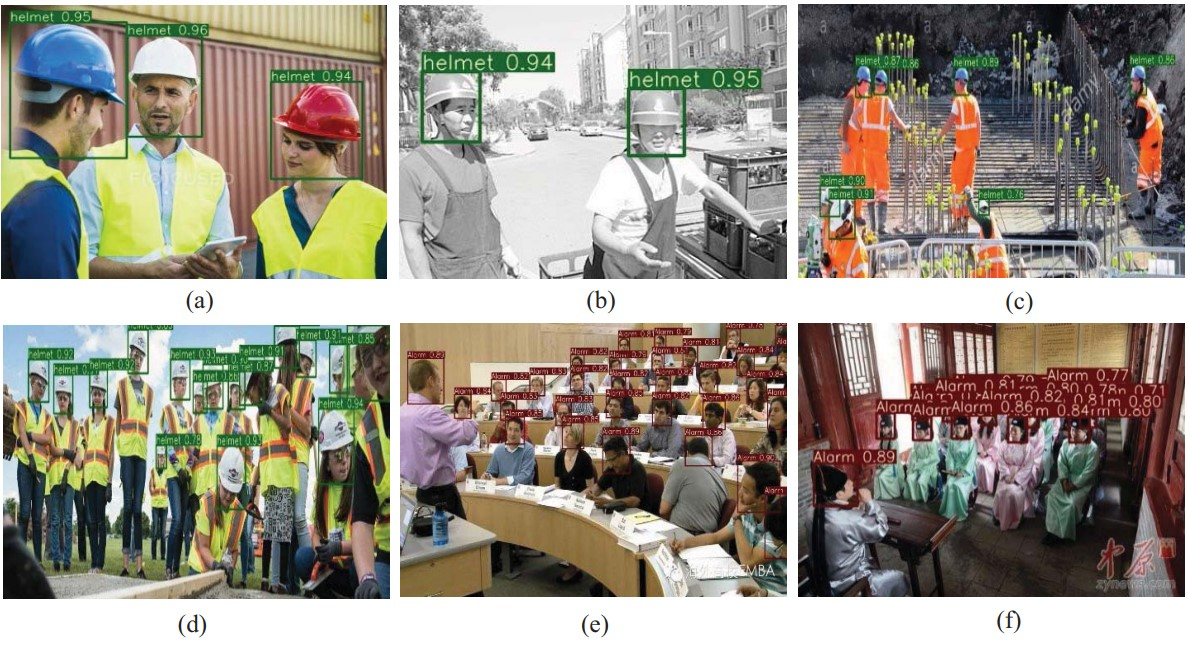
\includegraphics[scale=0.7]{gambar/zhou_le.jpg}
    \caption{Hasil Deteksi Helm Keselamatan Kerja pada penelitian oleh Zhou dan kawan - kawan}
    \label{fig:zhouimage}  
\end{figure}

\section{Helm Keselamatan Kerja}
\label{sec:helmkeselamatankerja}

\begin{figure}[ht]
    \centering
    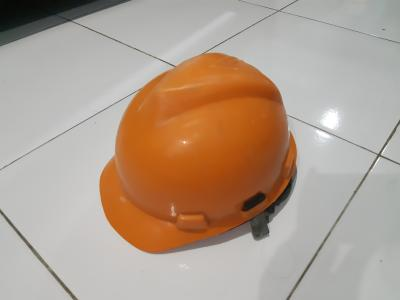
\includegraphics[width=1.0\textwidth]{gambar/safety_helmet.jpg}
    \caption{Helm Keselamatan Kerja}
    \label{fig:helmkeselamatankerja}  
\end{figure}

Helm Keselamatan Kerja seperti helm atau pelindung kepala pada umumnya memiliki kemampuan untuk 
melindungi kepala pengguna. Menurut surat dari Menteri Tenaga Kerja dan Trasmihrasi nomor PER. PER. 08/MENVIII/2010, 
jenis – jenis alat perlindungan diri salah satunya yaitu Alat Pelindung Kepala yang dimana contoh bentuk
nya yaitu helm keselamatan kerja atau safety helmet diantara alat pelindung lainnya \cite{suratkementriantenagakerja}. 
Saat digunakan dengan tepat, helm dapat menyerap dampak benturan yang mengurangi gaya yang disalurkan ke kepala hingga 10 persen dari dampak benturan aslinya. \cite{kim2018safety}

Badan Standar Dunia dari Amerika, \emph{Occupational Safety and Health Administration} atau OSHA mengatur 
standardisasi Helm Keselamatan Kerja di pedoman ANSI/ISEA Z89.1-2014. Dalam pedoman memiliki dua tipe 
klasifikasi perlindungan yaitu TIPE I yang merupakan perlindungan dari atas dan TIPE II yang merupakan 
perlindungan lateral atau menyamping yang dimana kedua tipe dites untuk benturan dan ketahanan dari 
penetrasi. Untuk tipe II meliputi kemampuan meredam benturan dari depan , belakang, dan samping. 
Selain itu TIPE II juga meliputi pertahanan penetrasi off-center dan ketahanan tali dagu \cite{american1997american}.

Selain dari 2 tipe perlindungan dari benturan, standardisasi ANSI/ISEA Z89.1-2014 juga meliputi 3 kelas tingkat isolasi listrik yaitu \cite{american1997american}:
\begin{enumerate}
    \item \emph{G Class} yang tahan sampai 2.200 volt
    \item \emph{E Class} yang tahan sampai 20.000 volt
    \item \emph{C Class} yang sama sekali tidak memiliki tingkat isolasi listrik
\end{enumerate}

Dari situ dapat disimpulkan bahwa helm keselamatan kerja memiliki manfaat yang besar dalam melindungi kepala personel konstruksi.

\newpage

\section{Peraturan Menteri Tenaga Kerja dan Transmigrasi Republik Indonesia tentang Alat Pelindung Diri}
\label{sec:peraturanapd}

\par Peraturan Menteri Tenaga Kerja dan Transmigrasi Republik Indonesia NOMOR PER.08/MEN/VII/2010 mengatur tentang alat pelindung diri.
Peraturan ini meliputi pihak - pihak yang terlibat, kewajiban penyediaan APD, peralatan yang termasuk APD, dan karakteristik tempat
yang diwajibkan APD \cite{suratkementriantenagakerja}. Pada pasal 3 ayat 1, disebutkan alat - alat yang termasuk sebagai alat pelindung diri
yaitu :

\begin{enumerate}[nolistsep]
    \item pelindung kepala
    \item pelindung mata dan muka
    \item pelindung telinga
    \item pelindung pernapasan beserta kelengkapannya
    \item pelindung tangan
    \item pelindung kaki
\end{enumerate}
Dimana pelindung kepala ini meliputi helm keselamatan kerja atau \emph{hardhat} \cite{suratkementriantenagakerja}.

\newpage

\section{Peraturan Menteri Pekerjaan Umum tentang Pedoman Sistem Manajemen Keselamatan dan Kesehatan Kerja (SMK3) Konstruksi Bidang Pekerjaan}
\label{sec:peraturansmk3}

\par Peraturan Menteri Pekerjaan Umum NOMOR : 05/PRT/M/2014 mengatur Pedoman Sistem Manajemen Keselamatan dan Kesehatan Kerja (SMK3) Konstruksi Bidang Pekerjaan.
Peraturan ini meliputi ketentuan umum tentang keselamatan dan kesehatan kerja konstruksi, sistem manajemen K3, pekerjaan konstruksi
,ahli K3 Konstruksi, petugas K3 Konstruksi, potensi bahaya, dan risiko K3. Dijelaskan pada pasal 6 ayat 1 dan 2 bahwa Ahli K3 atau Petugas K3 wajib dilibatkan pada konstruksi
dengan potensi bahaya tinggi atau rendah.

\section{Visi Komputer}
\label{sec:visikomputer}

\par Manusia bisa dengan mudahnya memahami struktur tiga dimensi yang ada di sekitarnya. Kita dapat mengetahui bahwa
sebuah balok memiliki ketebalan atau sebuah pot bunga yang memiliki isi. Kita juga dapat memahami benda yang semi transparan
seperti kantong plastik dimana cahaya matahari dapat menembus lembaran plastik tersebut. Lalu saat kita mengamati suatu kumpulan
barang - barang di gudang, kita juga dapat dengan mudahnya menentukan nama dari barang tersebut dan lokasinya. Begitu juga saat
mengamati foto keluarga yang terdiri dari banyak individu dimana kita dapat membedakan antara satu dengan yang lainnya bahkan hingga
emosi yang mereka perlihatkan lewat raut wajahnya. Peneliti sudah melakukan pengembangan



\par Visi Komputer adalah bidang ilmu yang mempelajari cara untuk memproses gambar terutama dalam meniru
kemampuan manusia dalam melihat. Kemampuan seperti rekognisi wajah hingga bentuk kemampuan lain yang bahkan
melebihi kemampuan manusia. Kebanyakan riset dari bidang visi komputer di \emph{deep learning} berfokus pada
pengenalan objek atau deteksi. Bentuknya dari pengenalan atau deteksi ini bisa meliputi membuat log atau laporan
objek apa saja yang ada dalam gambar hingga memberi penandaan pada objek yang terdeteksi \cite{Goodfellow-et-al-2016}. 


\section{\emph{Object Detection}}
\label{sec:objectdetection}

\par Deteksi Object atau \emph{Object Detection} dalam visi komputer sendiri adalah prosedur untuk mengklasifikasikan suatu objek
pada suatu gambar sekaligus berusaha untuk menentukan lokasi atau posisi dari objek yang ada pada gambar tersebut \cite{felzenszwalb2010object}. 
Manfaat dari \emph{Object Detection} yaitu dapat memberikan informasi terkait suatu gambar atau video agar bisa lebih dipahami yang lalu bisa dimanfaatkan
untuk berbagai bentuk aplikasi. Penelitian di bidang \emph{Object Detection} ini pada umumnya berjalan di area \emph{neural network} atau sistem \emph{machine learning}
yang lalu juga termasuk pembuatan algoritma \emph{neural network} untuk teknik deteksi objek. Tetapi deteksi pada suatu gambar memiliki banyak
hal yang perlu dipertimbangkan seperti arah sudut pandang, pencahayaan, objek yang menghalang, dan hal lainnya yang membuat 
deteksi objek dengan prediksi lokasi akurat semakin sulit untuk dilakukan \cite{zhao2019object}.

\section{Convolutional Neural Network}
\label{sec:convolutionalneuralnetwork}

\par \emph{Convolutional Neural Network} adalah metode deep learning yang didesain untuk rekognisi pada data dua 
dimensi yang dimana umumnya berupa gambar visual (tetapi tidak harus berupa gambar) dan untuk klasifikasi.
Convolutional Neural Network memiliki kedalaman jaringan yang tinggi sehingga juga bisa termasuk sebagai \emph{Deep Neural Network}.
Jika dibandingan dengan \emph{Multilayer Perceptron} atau MLP, kemampuan CNN untuk klasifikasi citra lebih baik dibandingkan dengan MLP karena MLP tidak memiliki
kemampuan untuk menyimpan \emph{spatial information} dari gambar dimana satu \emph{pixel} pada gambar dianggap sebagai satu fitur
terpisah atau independen \cite{putra2016klasifikasi}. \emph{Convolutional Neural Network} adalah bentuk \emph{deep neural network} yang tidak hanya
sekadar memiliki banyak \emph{layer} seperti konsep \emph{deep learning} tetapi juga meniru bagaimaimana cara otak manusia mengenali sebuah gambar \cite{kim2017convolutional}.

\par Sebelum adanya \emph{Convolutional Neural Network},pada \emph{image classification} atau \emph{recognition} dibuat sistem independen khusus yang hanya digunakan
untuk pengambilan fitur dari sebuah gambar dan tidak termasuk dari \emph{machine learning}-nya sendiri yang dimana membutuhkan waktu dan tenaga yang lebih. Selain itu, \emph{feature extractor}
independen ini juga tidak selalu menghasilkan performa yang stabil. 
Sistem \emph{fiture extradctor} independen ini digunakan sebelum dilakukan klasifikasi seperti yang ditunjukkan pada Gambar~\ref{fig:imgecog_beforeconv}.


\begin{figure}[ht]
    \centering
    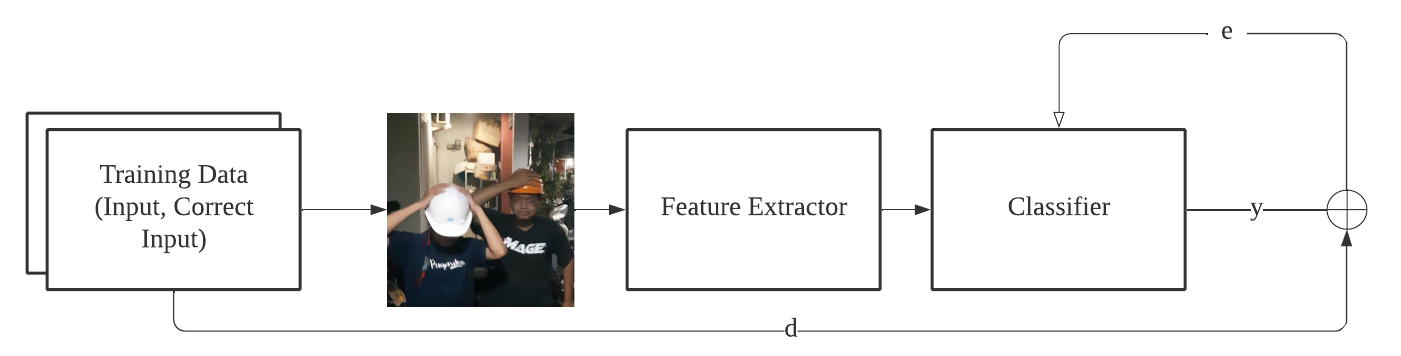
\includegraphics[width=1.0\textwidth]{gambar/imgrecog_beforconv.png}
    \caption{Sistem \emph{Feature Extractor} yang terpisah dari proses \emph{Machine Learning}}
    \label{fig:imgecog_beforeconv}  
\end{figure}

\par \emph{Convolutional Neural Network} mengikutsertakan proses pengambil fitur bersama dengan 
proses \emph{learning}-nya sendiri seperti yang ditunjukan pada Gambar~\ref{fig:imgrecog_afterconv}. Disinilah perbedaan dan kelebihan utama dari \emph{Convolutional Neural Network}
dimana CNN atau ConvNet ini secara \emph{automated} melakukan proses \emph{feature extraction} nya sendiri yang
menggunakan \emph{neural network} khusus yang \emph{weight} nya ditentukan melalui proses \emph{training} \cite{kim2018safety}.

\begin{figure}[ht]
    \centering
    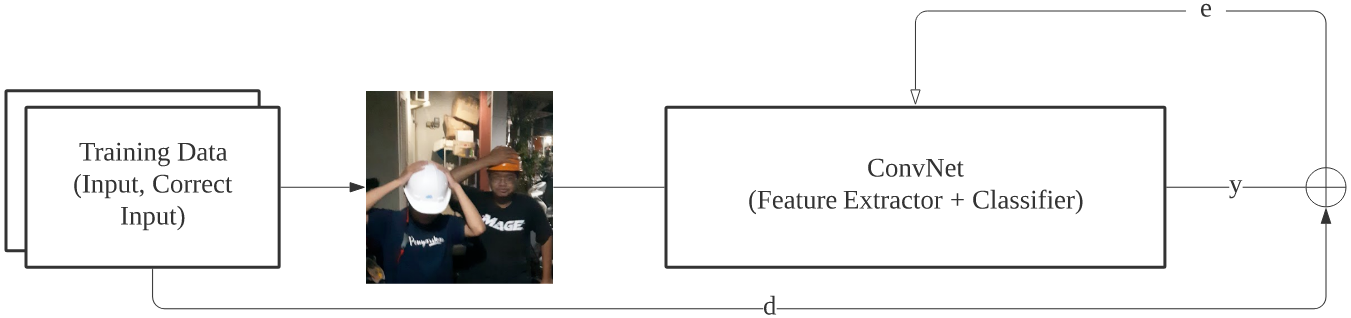
\includegraphics[width=1.0\textwidth]{gambar/imgrecog_afterconv.png}
    \caption{\emph{Feature Extractor} yang dilakukan bersama proses \emph{training} pada CNN}
    \label{fig:imgrecog_afterconv}  
\end{figure}



\par CNN dan MLP memiliki kemiripan dalam segi cara kerja. Perbedaan utama dari CNN dengan MLP adalah fakta
dimana CNN merepresentasikan neuron dalam bentuk 2D atau dua dimensi sedangkan pada MLP satu dimensi.
Seperti di MLP, CNN memiliki beberapa jumlah layer dengan masing - masing layer memiliki beberapa neuron.
Lalu masing - masing hubungan antar neuron di antara layer memiliki nilai bobot yang berada dalam bentuk empat dimensi
yang dimana merupakan kumpulan kernel konvolusi. Nilai bobot ini digunakan untuk melakukan operasi linear 
dari input yang dimana hasilnya ditransformasi untuk menjadi funsi aktivasi. Nama "\emph{Convolution}" pada 
CNN diambil dari operasi linearnya yang menggunakan operasi konvolusi \cite{putra2016klasifikasi}.
Pada arsitektur CNN, terdapat beberapa jenis layer yaitu \emph{Convolution Layer, Subsampling Layer, 
Fully Connected Layer}, dan \emph{Activation Layer}.

\subsection{\emph{Convolution Layer}}
\label{subsec:convolutionlayer}

\par \emph{Convolution Layer} yang merupakan layer utama dari CNN yang, sesuai namanya, melakukan proses konvolusi pada gambar 
yang lalu mengoutputkan \emph{feature map} yang dimana berguna untuk memunculkan fitur yang "unik" dari input gambar. Berbeda dengan layer pada
\emph{neural network} lainnya, \emph{convolutional layer} menggunakan \emph{convolutional filter} atau kernel untuk mengubah gambar input untuk proses konvolusi.
Kernel berkerja seperti memindai dari dari atas kiri ke kanan bawah gambar. Proses ini sebenarnya adalah aplikasi 
dari operasi konvolusi. Konvolusi merupakan pengaplikasian sebuah fungsi di suatu output secara berulang. Tujuan
diberlakukannya hal ini yaitu untuk mendapatkan fitur dari input gambar yang dimana konvolusinya akan menghasilkan
transformasi linear dari data. Bobot disini dapat diartikan sebagai spesifikasi dari kernel konvolusi yang digunakan yang
dimaksudkan untuk kernal dapat dilatih berdasarkan input yang diterima. Seperti yang diilustrasikan pada Gambar~\ref{fig:ilutrasikonvolusi} , diumpamakan sebuah
input gambar dalam bentuk matrix 5x5 berwarna hijau digunakan sebagai target konvolusi menggunakan kernel 3x3 yang diilustrasikan dengan
warna kuning dimana akan memindai dari atas kekanan bawah dengan operasi perkalian dan akan menghasilkan output hasil konvolusi yang
merupakan bentuk ektraksi fitur dari gambar input.

\begin{figure}[ht]
    \centering
    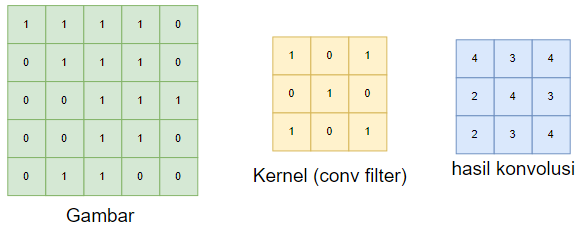
\includegraphics[width=1.0\textwidth]{gambar/convolution_simulation.png}
    \caption{Ilustrasi Konvolusi pada Matrix 5x5 dengan kernel 3x3}
    \label{fig:ilutrasikonvolusi}  
\end{figure}


\subsection{\emph{Subsampling Layer}}
\label{subsec:subsamplinglayer}

\par Subsampling Layer merupakan tahap atau proses reduksi ukuran data dari suatu gambar atau citra. Tujuannya selain mengecilkan
ukurannya yaitu meningkatkan invariasi dari posisi fitur. Pada umunya metode \emph{Max Pooling} yang sering digunakan pada proses sub sampling ini daripada \emph{Mean Pooling}.
Max Pooling membagi keluaran dari convolution layer menjadi grid kecil yang dimana disini diambil \emph{max value}-nya dari dari setiap grid
tadi yang digunakan untuk menyusun gambar citra yang sudah tereduksi seperti yang ditunjukan pada Gambar~\ref{fig:prosespooling}. Menurut Springenberg et al. \cite{springenberg2014striving}, pooling layer ini digunakan
untuk mereduksi gambar sehingga lebih mudah digantikan sebuah convolution layer dengan stride yang sama dengan pooling layer
bersangkutan\cite{putra2016klasifikasi}.

\begin{figure}[ht]
    \centering
    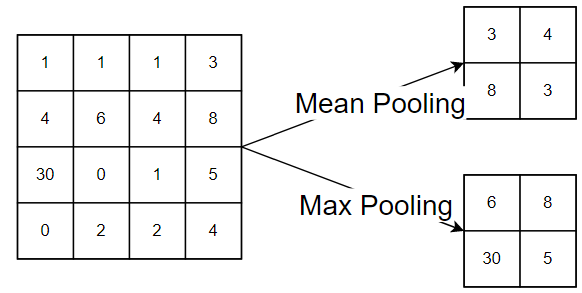
\includegraphics[width=1.0\textwidth]{gambar/pooling.png}
    \caption{Proses \emph{Max Pooling} dan \emph{Mean Pooling}}
    \label{fig:prosespooling}  
\end{figure}

\subsection{\emph{Fully Connected Layer}}
\label{subsec:fullyconnectedlayer}

\par \emph{Fully Connected Layer} digunakan untuk melakukan transformasi untuk dilakukan klasifikasi secara linear.
Neuron yang akan diinputkan ke FC layer ini harus ditransformasikan menjadi satu dimensi yang dimana
mengakibatkan FC layer ini hanya bisa diletakkan di akhir jaringan karena data kehilangan \emph{spatial information}-nya
sehingga menjadi \emph{irreversible} atau tidak bisa dikembalikan.

\subsection{\emph{Activation Layer}}
\label{subsec:activationlayer}

\par \emph{Activation Layer} adalah tempat dilakukannya fungsi aktivasi dimana dilakukan transformasi data input
menjadi dimensi tinggi agar memungkinakan untuk dilakukan klasifikasi \cite{putra2016klasifikasi}.



\section{\emph{You Only Look Once} (YOLO)}
\label{sec:youonlylookone}

\emph{You Only Look Once} atau YOLO adalah algoritma \emph{muti object detection} yang sangat cepat yang dicetuskan oleh Redmot et al pada tahun 2015
lewat buku mereka \emph{You Only Look Once: Unified, Real-Time Object Detection} \cite{redmon2016you}. \emph{Convolutional Neural Network} menjadi basis dari sistem deteksi YOLO ini.
YOLO melakukan deteksi objek dengan menganggap nya sebagai pemrasalahan regresi tunggal yang diambil langsung dari \emph{pixel - pixel} yang ada
di gambar menjadi \emph{bounding box} penanda dari koordinat - koordinat dan probabilitas dari klasifikasinya. Dengan begitu
hanya perlu dilakukan satu kali pengecekan pada gambar untuk melakukan deteksi atau indentifikasi. \cite{redmon2016you}
YOLO menggabungkan beberapa komponen dari teksi objek menjadi satu neural network yang dimana menggunakan fitu-fitur
dari seluruh bagian gambar untuk memprediksi tiap \emph{bounding box} sekaligus melakukan prediksi untuk semua
\emph{bounding box} di semua tipe klasifikasi yang ada. Desain dari YOLO ini memungkinkan untuk melakukan
\emph{end to end training} dan kecepatan deteksi \emph{real time}.

\par Sistem dari YOLO sendiri membagi input gambar menjadi grid S x S. Grid disini perannya untuk 
nanti yaitu jika grid tertentu menjadi pusat dari objek maka grid tersebut yang nantinya berguna untuk deteksi objek tadi.

\par Setiap grid memprediksi tiap bound box dan nilai kemungkinan klasifikasi atau \emph{confidence score} dari \emph{bounding box} tersebut.
Nilai tersebut mewakili seberapa "yakin" model akan objek yang terdeteksi di bounding box dan seberapa akurat
prediksinya. 

\par Terdapat lima nilai prediksi yang ada pada tiap bounding box yaitu : x, y, w, h, dan \emph{confidence}.
X dan Y mewakili pusat dari bounding box. W dan H mewakili \emph{Weight} dan \emph{Height} diprediksi relatif
dari seluruh gambar. Lalu \emph{confidence score} sendiri mewakili IOU antara \emph{predicted box} dan \emph{ground truth box} \cite{redmon2016you}.

\subsection{YOLOv5}
\label{subsec:yolov5}

\begin{figure}[ht]
    \centering
    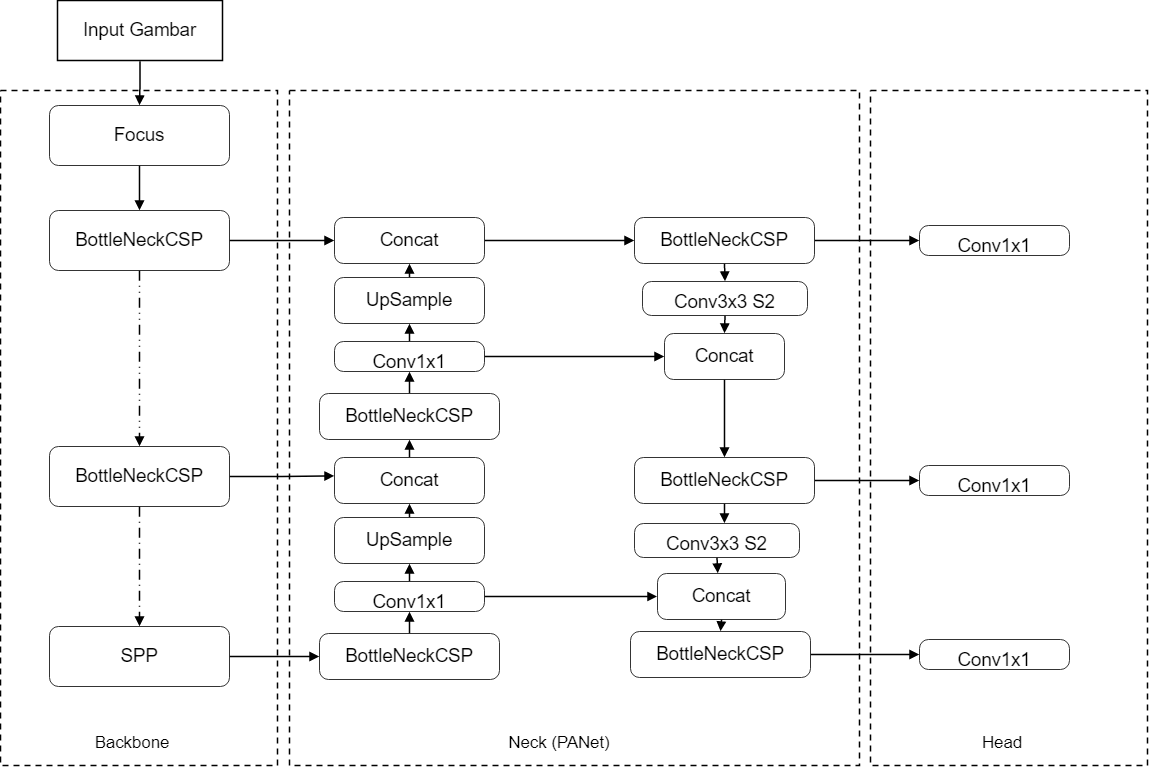
\includegraphics[width=1.0\textwidth]{gambar/yolov5 structure.png}
    \caption{Struktur Jaringan YOLOv5}
    \label{fig:yolov5network}  
\end{figure}

\par YOLOv5 merupakan versi pembaruan dari YOLO yang dicetuskan pada tahun 2020 oleh Glenn Jocher \cite{glenn_jocher_yolov5}. Berdasarkan dari \emph{repository} Github untuk YOLOv5 oleh Glenn Jocher, struktur jaringan dari YOLOv5 dibagi menjadi 3 bagian utama yaitu modul \emph{Backbone}, \emph{Neck}, dan \emph{Head}.
Seperti yang dapat dilihat di Gambar \ref{fig:yolov5network} Struktur jaringan dari YOLOv5 ini dimulai dari modul \emph{Backbone} dimana dilewati pertama oleh input gambar untuk mengekstrak fitur - fitur dari gambar yang strukturnya berbasis dari struktur \emph{Focus}, \emph{Bottleneck CSP (Cross Stage Partinal Networks)}, dan \emph{Spatial Pyramid Pooling (SPP)}.
Hasil ekstraksi fitur dari \emph{Backbone} lalu digunakan untuk menghasilkan \emph{feature pyramid} di modul \emph{Neck} yang merupakan struktur yang berbasis dari PANet (\emph{Path Aggregation Network}).
Lalu terakhir di Modul \emph{Head} dilakukan penampilan \emph{bounding box} yang meliputi beberapa informasi yaitu : kelas, koordinat, dan \emph{confidence score}.

  \cleardoublepage

  % Bab 3 desain dan implementasi
  \chapter{METODOLOGI}
\label{chap:metodologi}

% Ubah bagian-bagian berikut dengan isi dari desain dan implementasi

Judul penelitian "Deteksi Helm Keselamatan Kerja Menggunakan CNN" mengikuti metode atau desain sistem berikut serta impelementasinya.


\section{Peralatan}
\label{sec:peralatan}

Dalam pengerjaan judul tugas akhir ini, terdapat beberapa peralatan dan bahan yang digunakan dalam rangka menyelesaikan penelitian ini mulai dari tools berupa software atau perangkat lunak hingga hardware atau perangkat keras. Berikut pemaparan dari alat - alat yang digunakan.

\begin{enumerate}[nolistsep]
  \item Computer Desktop 
  \item Google Colab
\end{enumerate}

% \begin{table}[]
%   \begin{tabular}{|l|l|}
%     \caption{Conf 1}
%     \label{tb:asdadas}\\
%   \hline
%   Tipe               & Detail                                                              \\ \hline
%   \textit{Processor} & AMD Ryzen 5 2600                                                    \\ \hline
%   Memory             & 16 GB                                                               \\ \hline
%   Storage            & \begin{tabular}[c]{@{}l@{}}SSD 256 GB, 1 TB\\ HDD 1 TB\end{tabular} \\ \hline
%   Graphic Card       & NVIDIA GeForce GTX 1060 6GB                                         \\ \hline
%   Operating System   & Windows 10                                                          \\ \hline
%   \end{tabular}
% \end{table}

\begin{longtable}{|c|c|c|}
  \caption{Spesifikasi Komputer Desktop}
  \label{tb:spesifikasikomputer}\\
  \hline
  % \rowcolor[HTML]{C0C0C0}
  \textbf{Tipe} & \textbf{Detail}  \\
  \hline
  \textit{Processor} & AMD Ryzen 5 2600 \\ 
  Memory             & 16 GB  \\
  Storage            & HDD 1TB SSD 1,256 TB\\
  Graphic Card       & NVIDIA GeForce GTX 1060 6GB \\
  Operating System   & Windows 10     \\
  CUDA               & CUDA version 11.2    \\              
  \hline
\end{longtable}

% \subsection{Anaconda}
% \label{subsec:anaconda}

% Anaconda sendiri merupakan package distribution yang dibuat khusus untuk data science. Anaconda biasanya digunakan untuk membuat environment baru untuk mengisolasi proyek dan menginstall package untuk keperluan tertentu. Pada penelitian ini akan digunakan untuk membantu penulis dalam mengumpulkan package - package yang diperlukan untuk melakukan proses training dan pengembangan sistem.\cite{pankajmathur_2018}

% \subsection{Python}
% \label{subsec:python}

% Python sendiri adalah bahasa pemrograman high level yang sudah terinterpretasi dan berbasis objek. Struktur data yang sudah ada di dalam python dan penulisan syntax yang sederhana dan mudah dipahami dapat meningkatkan performa pengerjaan. Pada penelitian ini python digunakan karena merupakan bahasa pemrograman yang cocok untuk data science mengingat struktur data di python yang dinamis. Selain itu python juga sudah termasuk saat menginstall Anaconda \cite{python.org}

% \subsection{Visual Studio Code}
% \label{subsec:visualstudiocode}

% Visual Studio Code adalah source code editor yang ramah performa dan mudah digunakan untuk segala bentuk keperluan penulisan text sehari - harinya. Visual Code mendukung banyak bahasa pemrograman dan menyediakan fitur addons yang digunakan untuk mendownload package untuk berbagai macam kebutuhan berbeda. Pada penelitian ini Visual Studio Code digunakan untuk menulisa script python yang akan digunakan untuk training, pengembangan sistem, dan keperluan lainyna yang sekiranya dibutuhkan pada penelitian ini dan dapat diselesaikan dengan visual studio code.\cite{microsoft_2021}

% \subsection{Roboflow}
% \label{subsec:roboflow}

% Roboflow merupakan \emph{tools} yang membantu developer untuk mengolah segala keperluan untuk melakukan pengembangan di bidang visi komputer. Fasilitas yang ditawarkan oleh Roboflow meliputi : pengorganisasian dataset, pelabelan atau \emph{annotation} , pembagian rasio \emph{train/test}, \emph{preprocessing} yang meliputi re-size ukuran gambar, isolasi objek, grayscale, auto-adjust contrast, tile, dan bahkan sekaligus train. 


% \subsection{Google Colab}
% \label{subsec:googlecolab}

% Google Colab merupakan produk dari Google Research yang merupakan sarana penjalanan program Python menggunakan browser yang pada umumnya digunakan untuk keperluan machine learning, analisis data, dan pendidikan. Sebenarnya, Google Colab sendiri menggunakan Jupyter Notebook sebagai basisnya. Perbandingannya dengan Jupyter notebook yaitu penggunaan Google Colab tidak memerlukan banyak pe-nyetupan awal seperti pada Jupyter Notebook di komputer lokal. Google Colab juga memberikan fasilitas gratis kebutuhan computingnya termasuk penggunaan GPU. Tetapi terdapat limitasi - limitasi pada penggunaan Google Colab secara gratis seperti lama waktu penggunaan untuk GPU dan limitasi AFK saat menggunakannya. Tetapi batasan - batasan tersebut bisa lebih dilonggarkan lagi dengan berlangganan Google Colab Pro.

% Pada tugas akhir ini, Google Colab hanya digunakan untuk melakukan training untuk menghasilkan bobot - bobot menggunakan training dengan yolov5 untuk semua variasi tipe pre-trained dari yolov5, dan juga untuk mengeksport bobot yolov5 yang dihasilkan dalam format PyTorch menjadi format lain seperti ONNX atau TFLite yang dimana juga disedikana dari YOLOv5. Tetapi, Google Colab ini tidak digunakan untuk melakukan proses deteksi.

% \begin{enumerate}
%   \item Anaconda
%   \par 
%   \item Python
%   \item Visual Studio Code
%   \item Roboflow
%   \item Google Colab
% \end{enumerate}

\section{Desain Sistem}
\label{sec:desainsistem}

Judul untuk tugas akhir “Deteksi Helm Keselamatan Kerja Menggunakan CNN” ini berada dalam bidang computer vision atau visi komputer yang memiliki tujuan merancang sistem yang dapat mendeteksi penggunaan helm keselamatan kerja secara real-time. Menggunakan YOLOv5 yang merupakan versi terbaru dari YOLO (You Only Look Once) yang merupakan algoritma deteksi objek yang berbasis CNN (Convolutional Neural Network). Dataset yang digunakan berupa gambar - gambar personnel proyek yang mengenakan helm keselamatan kerja dan yang tidak. Gambar - gambar tersebut dikumpulkan dari beberapa sumber seperti dataset dari kaggle dan sumber lainnya.

\begin{figure}[ht]
  \centering
  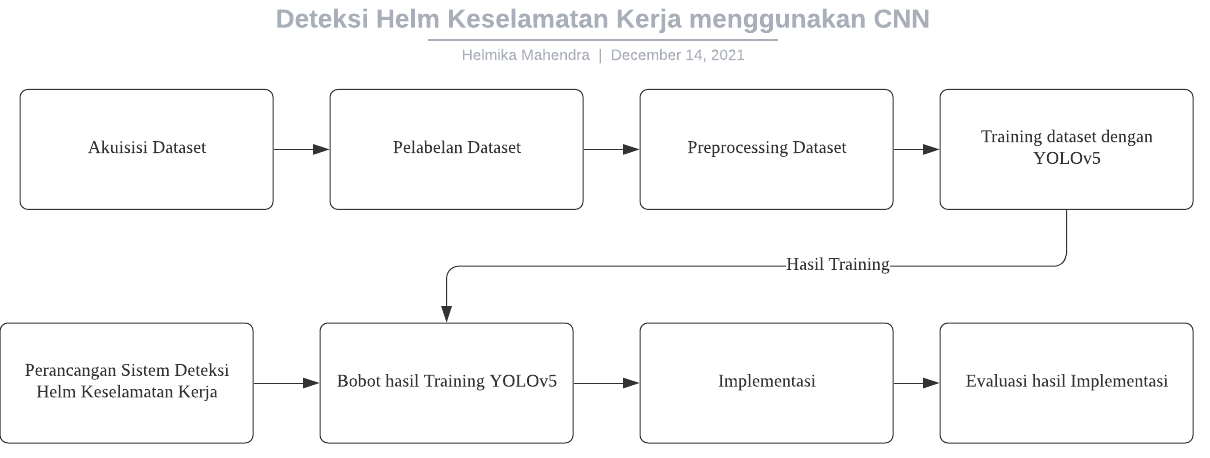
\includegraphics[scale=0.7]{gambar/Metodologi CNN.png}
  \caption{Bagan Umum Sistem}
  \label{fig:baganumumsistem}  
\end{figure}

\section{Alur Kerja}
\label{sec:alurkerja}

Prosedur pengerjaan dari judul tugas akhir ini dibagi menjadi beberapa tahap yang didasari dari metodologi yang sudah disusun seperti di gambar metodologi, yaitu :

\begin{enumerate}[nolistsep]
  \item Akuisi Dataset
  \item Pelabelan Dataset
  \item Preprocessing Dataset
  \item Training Dataset dengan Yolov5
  \item Perancangan Sistem Deteksi Helm Keselamatan Kerja
  \item Implementasi
  \item Evaluasi hasil implementasi
\end{enumerate}


\section{Akuisi Dataset}
\label{sec:akuisisidataset}

Dataset yang digunakan untuk training menggunakan Yolov5 berupa dataset berisi gambar - gambar yang mengandung personel lapangan proyek yang mengenakan helm dan yang tidak mengenakan helm. Untuk penelitian ini, dataset yang digunakan berasal dari dua sumber yaitu :

\begin{enumerate}
  \item Safety Helmet Detection oleh andrewmvd
  \par Dataset ini berisi 5000 gambar pekerja konstruksi yang meliputi orang yang menggunakan helm dan yang tidak menggunakan helm keselamatan kerja. Masin - masing
  gambar sudah diberi label ”helmet” dan ”head”. Format anotasi label nya berupa
  fromat PASCAL VOC yang disimpan dalam file .xml.   

  \begin{figure}[ht]
    \centering
    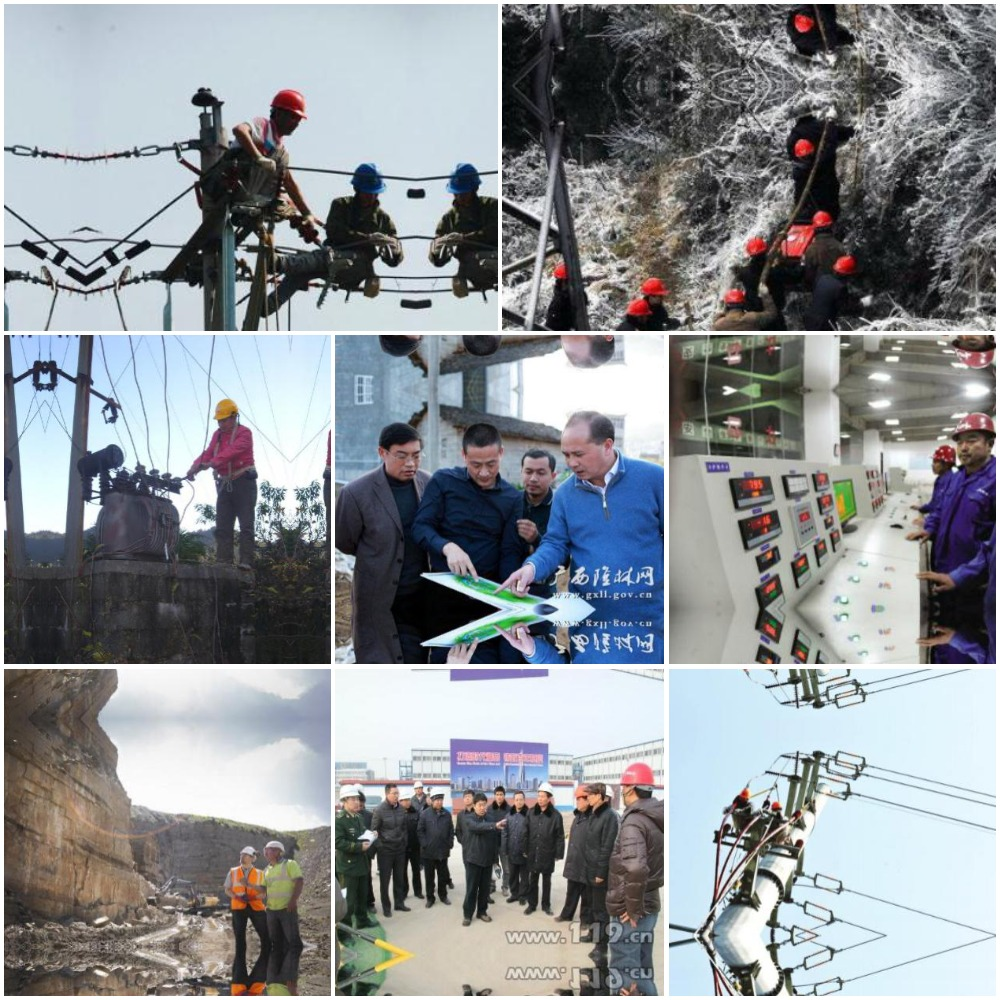
\includegraphics[scale=0.2]{gambar/safetyhelemtdataset_andrewmvd.png}
    \caption{Dataset \emph{Safety Helmet Detection} oleh andrewmvd}
    \label{fig:datasethelmetdetectionpreview}  
  \end{figure}

  \item SampleERASTY2020 dataset oleh Muhammad Aditya Wicaksono
  \par Dataset ini berisi 8.867 gambar yang kandungannya serupa dengan dataset Safety Helmet Detection oleh andrewmvd sebelumnya. Dataset ini juga sudah lengkap dengan annotasi nya tetapi membutuhkan beberapa perubahan untuk disesuaikan dengan  metode trainingnya. Selain itu, 8.867 gambar tersebut juga sudah termasuk hasil augmentasi seperti flip, rotation, blur, dan noise.
\end{enumerate}

\section{Pelabelan Dataset}
\label{sec:pelabelandataset}
Untuk keperluan training dan deteksi, terdapat 2 class :

\begin{enumerate}[nolistsep]
  \item "with\textunderscore helmet" yang meliputi kepala dan helm keselamatan kerja
  \item “no\textunderscore helmet” yang meliputi kepala tanpa helm keselamatan kerja
\end{enumerate}


Pada dataset yang sudah didapatkan sudah memiliki pelabelan atau anotasi nya masing - masing, tetapi khusus untuk dataset SampleERASTY2020 terdapat ketidak sesuaian untuk label Hard-hat  dimana hanya meliputi helm keselamatan kerja tanpa kepala penggunananya. Maka dari itu  dilakukan pelabelan ulang untuk dataset SampleERASTY2020 dimana hanya menggunakan file gambar yang masih belum hasil augmentasi yang berjumlah 338 gambar.

\begin{figure}[ht]
  \centering
  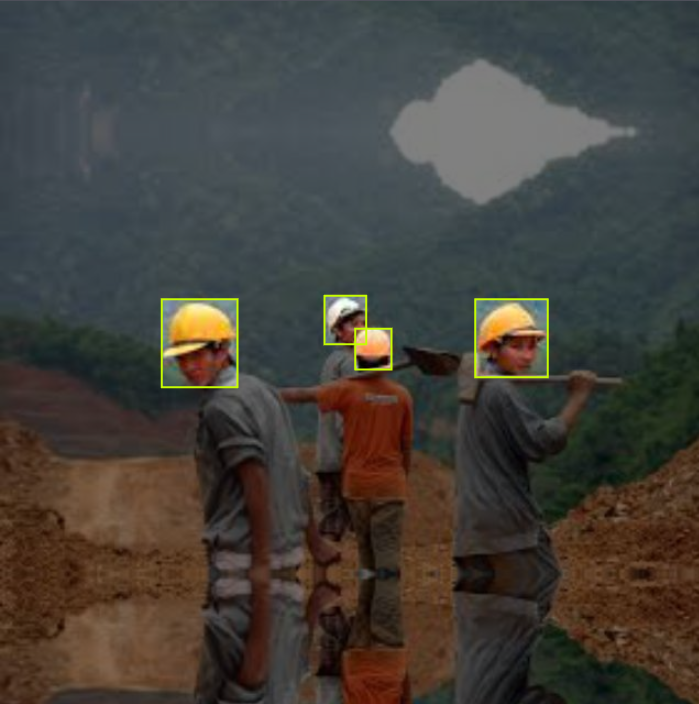
\includegraphics[scale=0.2]{gambar/Screenshot_87.png}
  \caption{Gambar beserta label}
  \label{fig:gambarbesertalabel}  
\end{figure}

\section{Preprocessing Dataset}
\label{sec:preprocessing}
Dataset yang sudah dikumpulkan lali digabungkan dan dilakukan preprocessing yang dimana untuk tahap ini penulis memanfaatkan Roboflow.
YOLOv5 yang digunakan untuk men-train dataset menerima gambar dalam ukuran 640x640 dengan warna RGB sehingga dataset yang ada akan diresize dalam ukuran tersebut. Source code YOLOv5 dari repository github sebenarnya sudah menyediakan fitur resize sebelum di train tetapi dari penulis melakukan resize menggunakan roboflow. 

Terdapat beberapa gambar yang tidak diperlukan dari dataset yang didapatkan seperti gambar yang hanya memiliki gambar rompi proyek yang dimana tidak digunakan untuk keperluan training. Untuk beberapa gambar tersebut akan tidak diikutkan dalam export dataset dari roboflow.

Penamaan kelas  label yang ada dari dataset yang sudah ada akan disesuaikan untuk keperluan penggunaan dan pemahaman yang lebih mudah. Dataset SampleERASTY2020 yang sudah dilabel ulang tidak perlu melewati proses ini tetapi untuk dataset Safety Helmet Detection perlu dilakukan penamaan ulang dimana untuk class “helmet” menjadi “with\textunderscore helmet” dan “head” menjadi “no\textunderscore helmet” seperti yang ditunjukan pada Gambar \ref{fig:labelbaru}. Augmentasi tambahan juga dilakukan pada dataset untuk menambah variasi gambar pada dataset dimana untuk bentuk augmentasi yang digunakan yaitu \emph{noise} dan \emph{horizontal flip}. Proses augmentasi dilakukan di platform \emph{Roboflow} yang juga menyediakan fitur augmentasi. Dataset SampleERASTY2020 yang sudah dilabel ulang dan diaugmentasi tambahan lali digabungkan dengan dataset yang sudah didapatkan sebelumnya yang berjumlah 5000 gambar. 

\begin{figure}[ht]
  \centering
  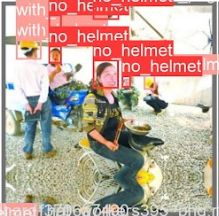
\includegraphics[scale=1]{gambar/Screenshot_86.png}
  \caption{Label baru}
  \label{fig:labelbaru}  
\end{figure}

Sebelum di export, dilakukan pembagian rasio file untuk train - test - validation. Pembagian nya yaitu 70\% train (4202) , 20\% test (1.200 gambar), dan 10\% validation (600 gambar). Untuk \emph{training} menggunakan YOLOv5 yang berbasis \emph{PyTorch}, \emph{Roboflow} menyediakan fitur \emph{export} dataset ke format yang ditentukan dimana disini anotasinya disimpan dalam bentuk \emph{.txt} dan diatur lewat file \emph{.yaml}. Lalu khusus untuk dataset SampleERASTY2020 yang sudah dilabel ulang, dilakukan beberapa augmentasi menggunakan roboflow. Augmentasi yang digunakan yaitu flip untuk horizontal dan vertikal diman menghasilkan 600 gambar tambahan. Lalu juga dilakukan augmentasi berupa noise 11\% yang menghasilkan tambahan 300 gambar.

Sebelum digunakan untuk men-\emph{traing} \emph{weight}, dataset yang sebelumnya sudah digabungkan perlu ditentukan pembagiannya untuk set \emph{train - test - val}-nya. Pembagian untuk dataset yang digunakan untuk training yaitu 70\% train (4202) , 20\% test (1.200 gambar), dan 10\% validation (600 gambar). Pembagian dataset ini dilakukan melalui fitur \emph{Generate Dataset Version} pada platform \emph{Roboflow}. 

\section{Training Dataset}
\label{sec:trainingdataset}

Dataset - dataset yang sudah di pre-process sebelumnya di roboflow dan sudah memiliki anotasi yang susai lalu digunakan untuk training menggunakan YOLOv5. Training ini merupakan proses pelatihan model dengan input gambar - gambar dari dataset yang sudah diberi anotasi dimana gambar dan anotasinya tersebut diolah hingga menghasilkan suatu karakteristik atau pola khusu dari kelas/label yang ditentukan sebelumnya lewat anotasi sehingga selanjutnya dapat digunakan komputer untuk menebak gambar yang nantinya dideteksi. Khusus untuk YOLOv5 yang menggunakan PyTorch sebagai framework machine learningnya, hasil training nya beruba bobot atau weight  akan diexport dalam bentuk .pt (format pytorch). 

\begin{longtable}{|c|c|c|}
  \caption{Konfigurasi Training menggunakan YOLOv5}
  \label{tb:konfigurasitrainingyolov5s}\\
  \hline
  \rowcolor[HTML]{C0C0C0}
  \textbf{Jenis Konfigurasi} & \textbf{Detail}  \\
  \hline
  \emph{batch\textunderscore size} & 16 \\
  \emph{epoch} & 150 \\
  \emph{imgsize} & 640\\
  \emph{data} & /content/yolov5/helmetDetection\textunderscore yolov5\textunderscore 2/data.yaml\\
  \emph{optimizer} & SGD (DEFAULT)\\
  \emph{device} & CUDA\\ 
  \emph{weights} & yolov5n, yolov5s, yolov5m, yolov5l\\ 
  \hline
\end{longtable}


Proses train dilakukan dengan batch size 16 dan 150 epoch dengan optimizer default untuk yolov5 yaitu SGD. Batch\textunderscore size disini menentukan jumlah gambar yang akan digunakan untuk train dalam satu iterasi, ditentukan 16 dengan pertimbangan limitasi hardware yang digunakan untuk proses training ini. Proses training dilakukan di Colab Pro dimana dengan limitasi GPU Ram yang diberikan, digunakan hingga mendekati 12 GB. Untuk image size sendiri algoritma yang sudah disediakan oleh YOLOv5 hanya menyiadakan resolusi 1:1 dimana dengan mengeset parameter imgsize 640 berarti ukuran untuk \emph{(height)} dan \emph{(width)} menjadi 640x640.

Proses training untuk judul ini tidak dilakukan dengan hardware komputer lokal melainkan memanfaatkan Google Colab Pro dimana proses trainingnya dijalankan secara cloud. 
Dataset yang sudah dikumpulkan sebelumnya didownload ke storage vm Colab Pro langsung dari Roboflow.  Dengan limitasi penggunaan storage, ram, dan GPU ram serta runtime yang diberikan google colab, dilakukan penyimpanan checkpoint untuk tiap epoch training di drive pribadi penulis. Hal dilakukan untuk kemungkinan jika sekiranya di tengah proses training session VM Colab Pro nya ter -terminate dengan sendirinya. 


\section{Perancangan Sistem Deteksi Helm Keselamatan Kerja}
\label{sec:perancangansistem}

\begin{figure}[ht]
  \centering
  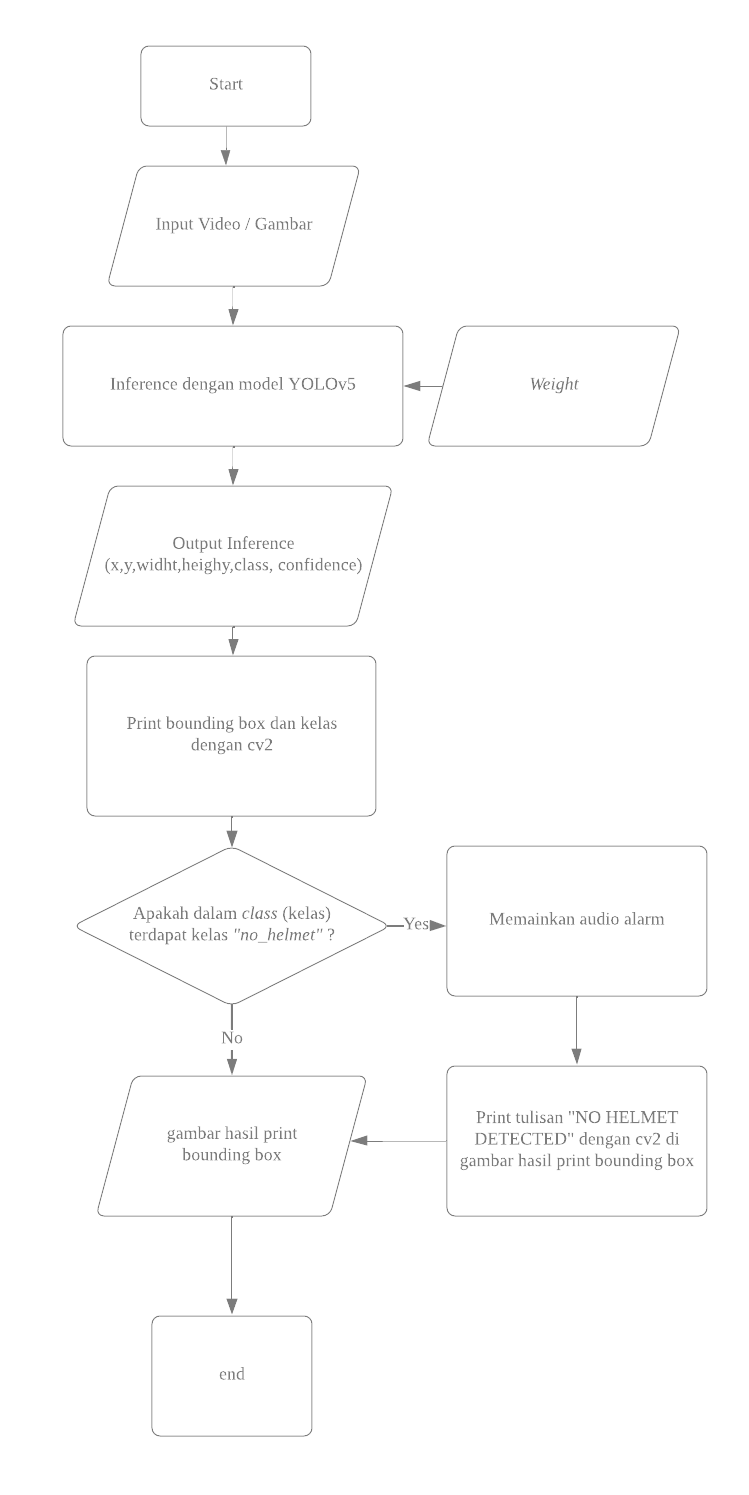
\includegraphics[scale=0.4]{gambar/flowchart_sistem.png}
  \caption{Flowchart Sistem Deteksi Helm Keselamatan Kerja}
  \label{fig:flchartdeteksi}  
\end{figure}

Sistem deteksi yang dibuat untuk Deteksi Helm Keselamatan kerja sendiri dikembangkan dari sistem deteksi yang sudah ada dari YOLOv5 dengan beberapa perubahan yang disesuaikan khusus untuk judul ini. Flowchart untuk sistem Deteksi Helm Keselamatan Kerja dapat dilihat pada Gambar~\ref{fig:flchartdeteksi} .

% Sistem yang dibuat direncanakan akan dijalankan di komputer yang sudah terinstall Python dan framework PyTorch atau ONNX dimana merupakan format yang dihasilkan dari training sebelumnya.

Sistem nya akan dibuat sebagai file script python yang dapat di run dan dapat menerima beberapa parameter : ukuran gambar, sumber input, dan bobot atau weight yang akan digunakan. 
Input yang dapat digunakan dengan script yang dibuat dapat dilakukan dalam bentuk gambar, file video, link youtube, link stream, dan feed camera dengan basis dari script detect.py dari YOLOv5. Tetapi, yang akan digunakan sebagai default nanti adalah feed dari kamera atau webcam yang tersedia di hardware yang digunakan untuk menjalankan inference. Ukuran atau resolusi gambar yang diterima sebagai ukuran default yaitu 640x640. 

% Untuk kasus jika input berupa gambar tunggal, gambar tersebut akan digunakan untuk inference melalu model yolov5 dengan bobot yang sudah dibuat sebelumnya lalu hasil inference yolov5 akan menghasilkan beberapa output. Tetapi untuk sistem yang akan dijalankan akan memanfaatkan feed dari camera atau webcam secara realtime sehingga akan dilakukan inference untuk tiap frame yang masuk dari input webcam.

Tiap frame yang masuk dari input \emph{webcam} akan digunakan untuk proses \emph{inference} melalui model \emph{yolov5} dengan \emph{weight} yang sudah dibuat sebelumnya melalui proses training. Hasil dari \emph{inference} menggunakanm \emph{YOLOv5} akan menghasilkan input berupa posisi untuk objek yang dideteksi yaitu \emph{xcenter, ycenter} serta dimensi dari objeknya yaitu \emph{widht} dan \emph{height} serta informasi nama \emph{class} dan \emph{confidence\textunderscore score} untuk tiap objek yang dideteksi. Hasil \emph{output inference} yang didapat lalu digunakan untuk menggambar \emph{bounding box} pada \emph{frame} gambar yang sedang di\emph{inference} seperti pada Gambar~\ref{fig:outputboundingbox}.

\begin{figure}[ht]
  \centering
  
\includegraphics[scale=1]{gambar/bounding_box.png}
  \caption{Output Bounding Box}
  \label{fig:outputboundingbox}
\end{figure}

% Output yang dikeluarkan dari hasil inferensi menggunakan yolov5 yaitu xcenter, ycenter, width , height, confidence, dan class. Untuk keperluan menampilkan bounding box akan menggunakan xcenter, ycenter, width, dan height yang didapatkan dari output inference yang lalu dilengkapi dengan menampilkan nama class dan confidence score dari inferencenya. 

% Untuk fungsi trigger alarm jika terdeteksi adanya orang yang tidak menggunakan helm, untuk hasil output yang dihasilkan dari inference satu frame akan dicheck sekiranya mengandung class “no\textunderscore helmet” yang jika terpenuhi akan  menjalankan perintah untuk mengeprint “NO HELMET DETECTED” pada display dan menjalankan audio alarm. 

Fungsi alarm akan dijalankan ketika dalam frame yang sedang di-\emph{inference} terdeteks objek dengan \emph{class} bernama \emph{“no\textunderscore helmet”}. Fungsi alarm ini berisi perintah untuk memainkan audio alarm untuk mensimulasikan sirine alarm. Selain menjalankan fungsi alarm, akan juga dijalanan perintah untuk mendisplay text \emph{“NO HELMET DETECTED”} pada frame yang sedang di-\emph{inference}.

\begin{figure}[ht]
  \centering
  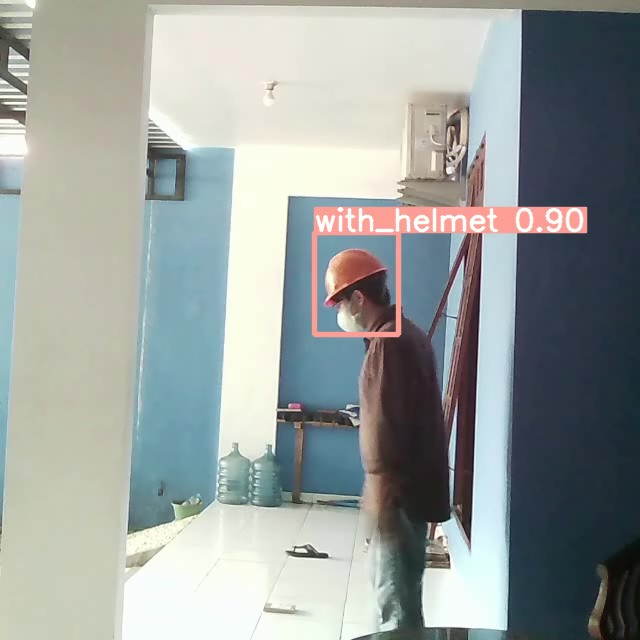
\includegraphics[scale=0.3]{gambar/video2_Moment.jpg}
  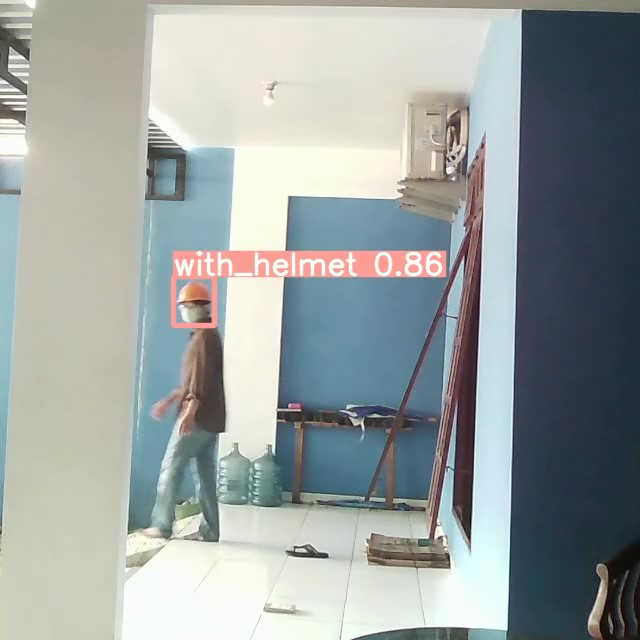
\includegraphics[scale=0.3]{gambar/video2_Moment2.jpg}
  \caption{Proses Deteksi Menggunakan Helm Keselamatan Kerja}
  \label{fig:deteksiwthhelm} 
\end{figure}

\begin{figure}[ht]
  \centering
  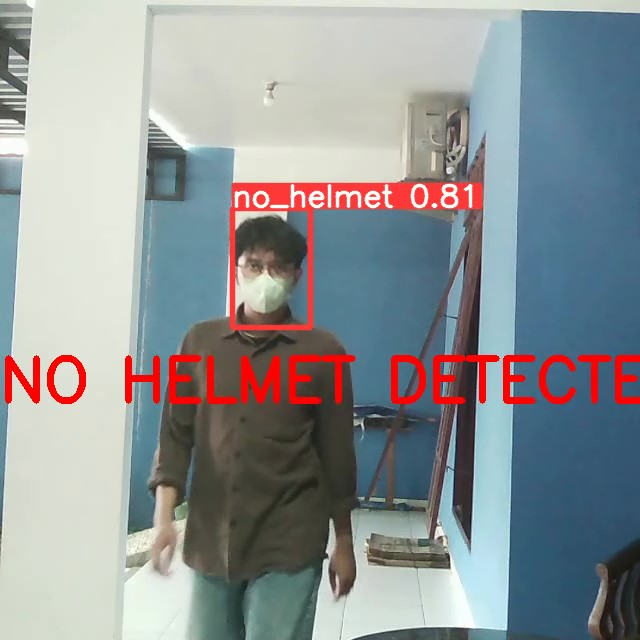
\includegraphics[scale=0.3]{gambar/video1_Moment.jpg}
  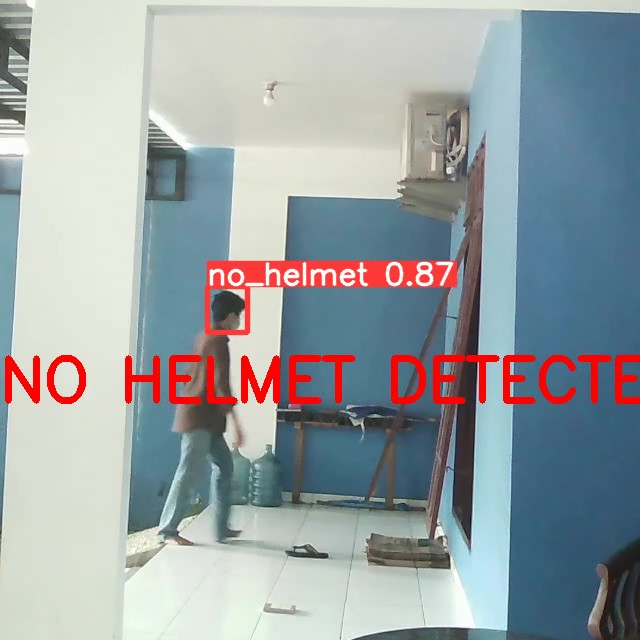
\includegraphics[scale=0.3]{gambar/video1_Moment2.jpg}
  \caption{Proses Deteksi Tidak Mengenakan Helm Keselamatan Kerja}
  \label{fig:deteksinohelm}  
\end{figure}

% Per blok diagram dijelaskan dan dibuatkan section masing-masing

% \section{Blok Diagram}
% \label{sec:blokdiagram}

% Contoh pembuatan potongan kode
% \begin{lstlisting}[
%   language=C++,
%   caption={Program halo dunia.},
%   label={lst:halodunia}
% ]
% #include <iostream>

% int main() {
%     std::cout << "Halo Dunia!";
%     return 0;
% }
% \end{lstlisting}

% \lipsum[2-3]

% % Contoh input potongan kode dari file
% \lstinputlisting[
%   language=Python,
%   caption={Program perhitungan bilangan prima.},
%   label={lst:bilanganprima}
% ]{program/bilangan-prima.py}

% \lipsum[4]

  \cleardoublepage

  % Bab 4 pengujian dan analisis
  \chapter{HASIL DAN PEMBAHASAN}
\label{chap:hasilpembahasan}

% Ubah bagian-bagian berikut dengan isi dari hasil dan pembahasan

Bab ini akan membahas hasil dan analisa dari desain sistem yang sudah dibuat dan implementasinya. Pengujian terhadap hasil dibagi menjadi beberap bagian.

\section{Pengujian Performa antar \emph{Weight}}
\label{sec:ujiperforma}
\par Repositori YOLOv5 menyediakan beberapa \emph{checkpoint} atau \emph{weight} yang merupakan hasil training model YOLOv5 dari dataset COCO yang dimanfaatkan sebagai \emph{pretrained model}. Ekspektasi penggunaan pretrained model ini yaitu bobot yang dihasilkan akan memiliki performa yang lebih tinggi daripada melakukan training tanpa pretrained model sama sekali. \emph{COCO Dataset} ini memiliki 80 \emph{class} berbeda. Seperti disebutkan pada \ref{sec:pelabelandataset} yaitu untuk keperluan penelitian ini hanya memerlukan 2 kelas yaitu "no\textunderscore helmet" dan "with\textunderscore helmet". 

\par Beberapa \emph{pretrained model} yang disedikana dari repositori YOLOv5 yaitu YOLOv5n, YOLOV5s, YOLOv5m, YOLOv5l,YOLOv5l, dan YOLOv5x. Selain beberapa model pretrained tersebut juga ada versi untuk ukuran gammbar 1280 yaitu seri YOLOv5n6 hingga YOLOv5l6. Pada penelitian ini hanya menggunakan variasi YOLOv5n hingga YOLOv5l karena variasi YOLOv5x dan versi seri 6 untuk ukuran gambar 1280 membutuhkan waktu yang lebih lama. Perbedaan - perbedaan yang ada pada bobot - bobot pretrained tersebut berasal dari konfigurasi awal dari training pada dataset COCO yang menggunakan YOLOv5, terutama pada paramter "depth\textunderscore multiple" dan "width\textunderscore multiple".

\par Proses validasi hasil training dilakukan menggunakan dataset Deteksi Helm Keselamatan Kerja yang pembagiannya dijelaskan pada bagian \ref{sec:preprocessing} yang berjumlah 1200 gambar dengan kelas "no\textunderscore helmet" berjumlah 1322 label dan kelas "with\textunderscore helmet" berjumlah 4294 label.

\par Pada bagian ini akan dipaparkan dan dibandingkan performa antara tiap bobot yang dihasilkan dengan model pretrained dan yang tidak menggunakan pretrained model. Pengujian ini dilakukan menggunakan \emph{resource} dari Google Colab. Spesifikasi \emph{resource} Google Colab yang digunakan saat melakukan validasi untuk bobot yang sudah di-\emph{train} dapat dilihat pada Tabel~\ref{tb:spekgoogleclab}.

\begin{table}
  \centering
  \caption{Spesifikasi \emph{Resource} Google Colab Untuk Validasi \emph{Weight}}
  \label{tb:spekgoogleclab}
  \begin{tabular}{|l|l|} 
  \hline
  Tipe    & Keterangan                      \\ 
  \hline
  Python  & Python-3.7.13                   \\
  PyTorch & torch-1.11.0+cu113              \\
  GPU     & Tesla P100-PCIE-16GB, 16281MiB  \\
  \hline
  \end{tabular}
\end{table}

\subsection{Pengujian Performa \emph{Weight} dari Hasil \emph{Pretrain} COCO Dataset}
\label{subsec:ujiperforma_coco}

\par Berikut merupakan pemaparan dari hasil validasi untuk bobot yang dilatih menggunakan \emph{pretrained weights}
dari YOLOv5 untuk varian \emph{Nano (N), Small (S), Medium(M),} dan \emph{Large(L)}. Hasil validasi dapat dilihat pada
Tabel~\ref{tb:pretraincoco}.


\begin{longtable}{|l|l|l|l|l|l|l|} 
  \caption{Hasil Validasi \emph{Weight} dari Hasil Pretrain}
  \label{tb:pretraincoco}\\
  \hline
  Nama Bobot                          & class        & precision & recall & mAP   & mAP .5:.95 & inference time (ms)    \\ 
  \hline
  \multirow{3}{*}{hedec\_pretrain\_N} & all          & 0.925     & 0.871  & 0.922 & 0.557      & \multirow{3}{*}{1.9}   \\
                                      & no\_helmet   & 0.924     & 0.867  & 0.916 & 0.552      &                        \\
                                      & with\_helmet & 0.926     & 0.875  & 0.929 & 0.562      &                        \\ 
  \hline
  \multirow{3}{*}{hedec\_pretrain\_S} & all          & 0.929     & 0.878  & 0.929 & 0.568      & \multirow{3}{*}{4}     \\
                                      & no\_helmet   & 0.925     & 0.857  & 0.918 & 0.561      &                        \\
                                      & with\_helmet & 0.932     & 0.9    & 0.941 & 0.575      &                        \\ 
  \hline
  \multirow{3}{*}{hedec\_pretrain\_M} & all          & 0.923     & 0.891  & 0.933 & 0.57       & \multirow{3}{*}{8.7}   \\
                                      & no\_helmet   & 0.919     & 0.883  & 0.923 & 0.561      &                        \\
                                      & with\_helmet & 0.928     & 0.898  & 0.943 & 0.58       &                        \\ 
  \hline
  \multirow{3}{*}{hedec\_pretrain\_L} & all          & 0.919     & 0.867  & 0.919 & 0.579      & \multirow{3}{*}{14}    \\
                                      & no\_helmet   & 0.904     & 0.846  & 0.899 & 0.565      &                        \\
                                      & with\_helmet & 0.934     & 0.887  & 0.939 & 0.593      &                        \\ 
  \hline
\end{longtable}

\begin{figure} [h!]
  \centering
  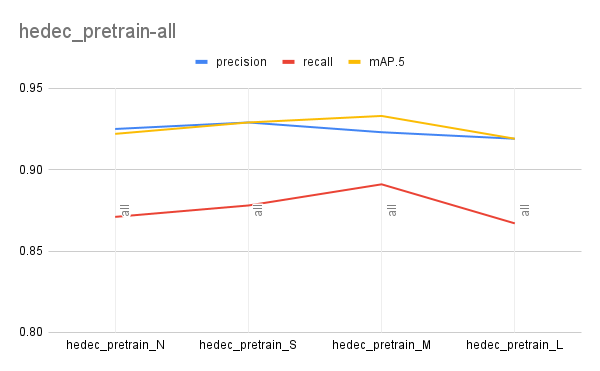
\includegraphics[width=1\textwidth]{gambar/final_weight_val/hedec_pretrain-all.png}
  \caption{Grafik \emph{Precision, Recall, mAP} untuk Bobot Hasil Pretrain COCO-YOLOv5 untuk Semua Kelas}
  \label{fig:grafval_pretrain_all}  
\end{figure}

\begin{figure} [h!]
  \centering
  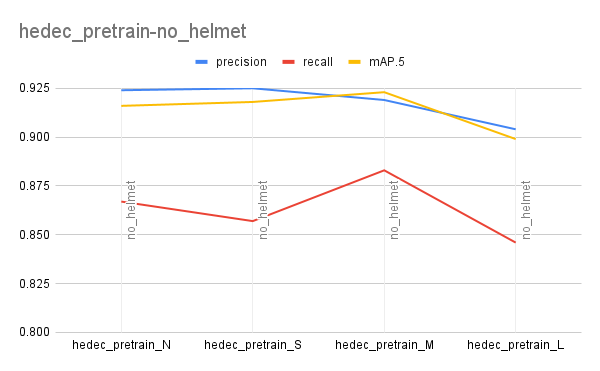
\includegraphics[width=0.49\textwidth]{gambar/final_weight_val/hedec_pretrain-no_helmet.png}
  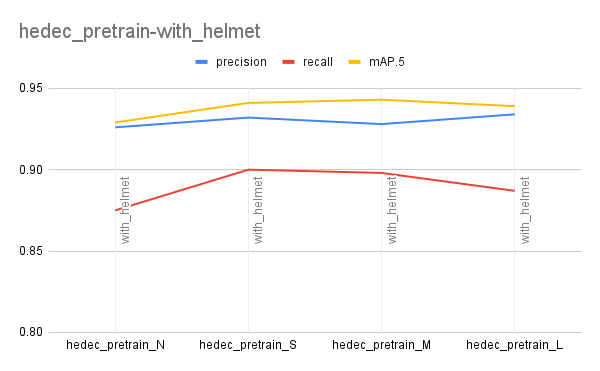
\includegraphics[width=0.49\textwidth]{gambar/final_weight_val/hedec_pretrain-with_helmet.png}
  \caption{Grafik \emph{Precision, Recall, mAP} untuk Bobot Hasil Pretrain COCO-YOLOv5 untuk Masing Masing Kelas}
  \label{fig:grafval_pretrain_eachclass}  
\end{figure}


\par Berdasarkan hasil validasi yang dipaparkan, tidak ada perbedaan signifikan dari \emph{precision, recall, mAP} 
baik pada kelas "with\_helmet" ataupun "no\_helmet" seperti yang ditunjukan pada Gambar~\ref{fig:grafval_pretrain_eachclass}.
Untuk nilai \emph{precision} berada di atas 0.9 dengan nilai tertinggi oleh varian "hedec\_pretrain\_S" . Untuk \emph{recall}
juga tidak terlalu berbeda diantara bobot dimana semuanya berada diatas angka 0.8 dengan bilai teringgi 
oleh varian "hedec\_pretrain\_M". 

\subsection{Pengujian Performa \emph{Weight} Hasil Train Murni Dataset Deteksi Helm Keselamatan Kerja}
\label{subsec:murnidataset}

\par Berikut merupakan pemaparan dari hasil validasi untuk bobot yang dilatih tanpa \emph{pretrained weights}
dari YOLOv5 . Tetapi untuk konfigurasinya dibuat serupa dengan varian \emph{Nano (N), Small (S), Medium(M),} dan \emph{Large(L)}. 
Hasil validasi dapat dilihat pada Tabel~\ref{tb:nopretrain}.


\begin{longtable}{|l|l|l|l|l|l|l|} 
  \caption{hasil Validasi \emph{Weight} dari Murni Dataset}
  \label{tb:nopretrain}\\
  \hline
  Nama Bobot                          & class        & precision & recall & mAP   & mAP .5:.95 & inference time (ms)    \\ 
  \hline
  \multirow{3}{*}{hedec\_pure\_N}     & all          & 0.918     & 0.848  & 0.909 & 0.532      & \multirow{3}{*}{1.9}   \\
                                      & no\_helmet   & 0.919     & 0.839  & 0.903 & 0.52       &                        \\
                                      & with\_helmet & 0.918     & 0.856  & 0.915 & 0.544      &                        \\ 
  \hline
  \multirow{3}{*}{hedec\_pure\_S}     & all          & 0.926     & 0.866  & 0.919 & 0.555      & \multirow{3}{*}{4.2}   \\
                                      & no\_helmet   & 0.925     & 0.86   & 0.911 & 0.55       &                        \\
                                      & with\_helmet & 0.927     & 0.872  & 0.927 & 0.559      &                        \\ 
  \hline
  \multirow{3}{*}{hedec\_pure\_M}     & all          & 0.932     & 0.866  & 0.924 & 0.564      & \multirow{3}{*}{8.9}   \\
                                      & no\_helmet   & 0.937     & 0.856  & 0.917 & 0.562      &                        \\
                                      & with\_helmet & 0.927     & 0.877  & 0.93  & 0.566      &                        \\ 
  \hline
  \multirow{3}{*}{hedec\_pure\_L}     & all          & 0.922     & 0.876  & 0.923 & 0.566      & \multirow{3}{*}{14.1}  \\
                                      & no\_helmet   & 0.919     & 0.868  & 0.914 & 0.561      &                        \\
                                      & with\_helmet & 0.925     & 0.884  & 0.932 & 0.572      &                        \\
  \hline
\end{longtable}

\begin{figure} [h!]
  \centering
  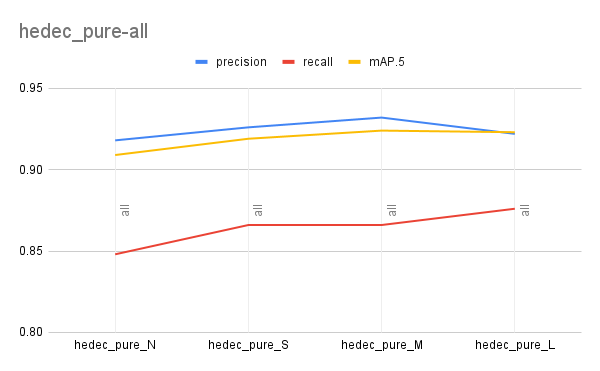
\includegraphics[width=1\textwidth]{gambar/final_weight_val/hedec_pure-all.png}
  \caption{Grafik \emph{Precision, Recall, mAP} untuk Bobot Tanpa Pretrain COCO-YOLOv5 untuk Semua Kelas}
  \label{fig:grafval_pure_all}  
\end{figure}

\begin{figure} [h!]
  \centering
  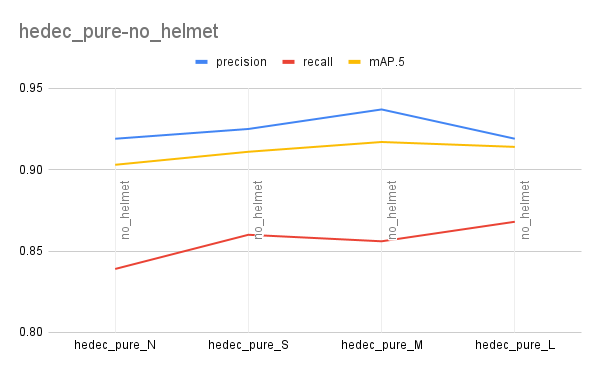
\includegraphics[width=0.4\textwidth]{gambar/final_weight_val/hedec_pure-no_helmet.png}
  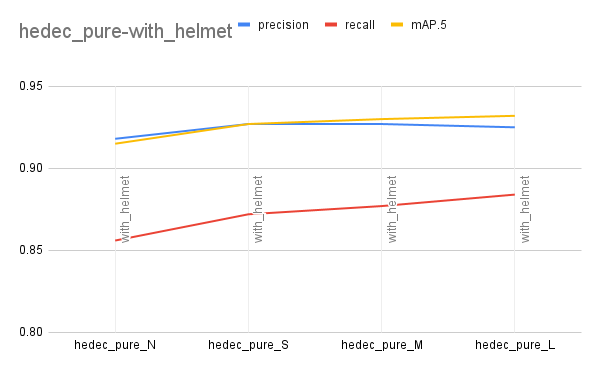
\includegraphics[width=0.4\textwidth]{gambar/final_weight_val/hedec_pure-with_helmet.png}
  \caption{Grafik \emph{Precision, Recall, mAP} untuk Bobot Tanpa Pretrain COCO-YOLOv5 untuk Kelas "no\_helmet"}
  \label{fig:grafval_pure_eachclass}  
\end{figure}

 
\newpage
\par Berdasarkan hasil validasi yang dilakukan untuk bobot - bobot yang dilatih tanpa menggunakan \emph{Pretrained Weights} dari YOLOv5
yang dapat ditarik beberapa point.Seperti yang dapat dilihat Gambar~\ref{fig:grafval_pure_all} untuk rata- rata semua kelas
dan Gambar~\ref{fig:grafval_pure_eachclass} untuk masing-masing kelas, ntuk \emph{precision} secara umum berada di atas 0.9 dan \emph{recall} di atas 0.8, begitu juga dengan
mAP.5 nya yang berada ditas 0.9. Tetapi dari segi \emph{inference time} untuk masing - masin varian, tidak ada perbedaan jauh jika dibandingkan
bobot - bobot yang di latih menggunakan \emph{Pretrained Weights} dari YOLOv5 yang dijelaskan di Sub Bab~\ref{subsec:ujiperforma_coco}.

\section{Pengujian Performa Berdasarkan Jarak}
\label{sec:ujiberdasarkanjarak}

Pada bagian ini akan memaparkan hasil deteksi pada dataset validasi yang dibagi menjadi beberapa variasi jarak dari kamera. Dataset yang digunakan meliputi 8 foto untuk masing - masing jarak.

\subsection{Pengujian Jarak dengan \emph{Pretrained Weight}}
\label{subsec:ujijarak_pretrainedweight}

\par Bagian ini memaparkan pengujian menggunakan bobot hasil \emph{training} menggunakan \emph{Pretrained Weights}
dari repo YOLOv5 yang selanjutnya disebut sebagai "hedec\_pretrain". 

\begin{enumerate}
  \item \textbf{hedec\_pretrain\_N}
  
  \par Pada pengujian menggunakan bobot "hedec\_pretrain\_N" pada perbedaan jarak seperti yang bisa dilihat di Gambar~\ref{fig:grafvaljarak_hedec_pretrain_N}, memiliki nilai
  \emph{precision} menurun mulai dari jarak 4 meter hingga 9 meter. Hal ini dikarenakan bobot ini salah memprediksi kelas "no\_helmet" sebagai "with\_helmet" pada jarak 4 meter
  dan selebihnya. Nilai \emph{recall} pada untuk kelas "no\_helmet" rendah pada jarak 1.3 meter karena ada kelas "no\_helmet" yang
  gagal diprediksi pada jarak 1.3 meter. Hasil validasi untuk bobot "hedec\_pretrain\_N" pada semua jarak dan kelas dapat dilihat pada Tabel~\ref{tb:hasiljarak_hedec_pretrain_N}

  \begin{figure} [h!]
    \centering
    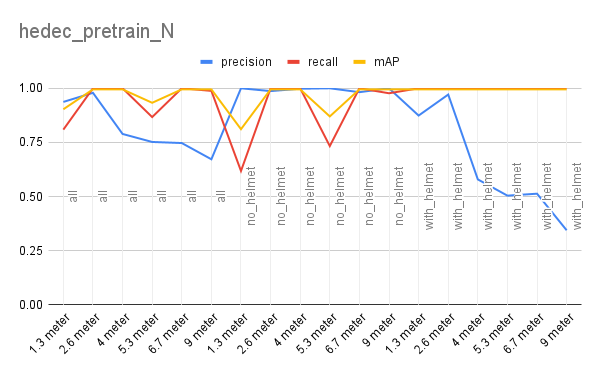
\includegraphics[width=1\textwidth]{gambar/BerdasarkanJarak/hedec_pretrain_N.png}
    \caption{Grafik \emph{Precision, Recall, mAP} untuk \textbf{"hedec\_pretrain\_N"} Pada Jarak 1.3 meter Hingga 9 meter}
    \label{fig:grafvaljarak_hedec_pretrain_N}  
  \end{figure}

 

  \begin{longtable}{|l|l|l|l|l|} 
    \caption{Hasil Validasi Perbedaan Jarak Pada \textbf{"hedec\_pretrain\_N"}}
    \label{tb:hasiljarak_hedec_pretrain_N}\\
    \hline
    Jarak     & class        & precision & recall & mAP    \\ 
    \hline
    \endhead
    1.3 meter & all          & 0.687     & 0.827  & 0.891  \\
    2.6 meter & all          & 0.981     & 1      & 0.995  \\
    4 meter   & all          & 0.826     & 0.988  & 0.995  \\
    5.3 meter & all          & 0.874     & 0.994  & 0.995  \\
    6.7 meter & all          & 0.858     & 0.991  & 0.995  \\
    9 meter   & all          & 0.63      & 0.933  & 0.995  \\
    1.3 meter & no\_helmet   & 1         & 0.655  & 0.995  \\
    2.6 meter & no\_helmet   & 0.989     & 1      & 0.995  \\
    4 meter   & no\_helmet   & 1         & 0.976  & 0.995  \\
    5.3 meter & no\_helmet   & 1         & 0.989  & 0.995  \\
    6.7 meter & no\_helmet   & 1         & 0.983  & 0.995  \\
    9 meter   & no\_helmet   & 1         & 0.866  & 0.995  \\
    1.3 meter & with\_helmet & 0.374     & 1      & 0.787  \\
    2.6 meter & with\_helmet & 0.973     & 1      & 0.995  \\
    4 meter   & with\_helmet & 0.651     & 1      & 0.995  \\
    5.3 meter & with\_helmet & 0.747     & 1      & 0.995  \\
    6.7 meter & with\_helmet & 0.716     & 1      & 0.995  \\
    9 meter   & with\_helmet & 0.26      & 1      & 0.995  \\
    \hline
  \end{longtable}

  \begin{figure} [h!]
    \centering
    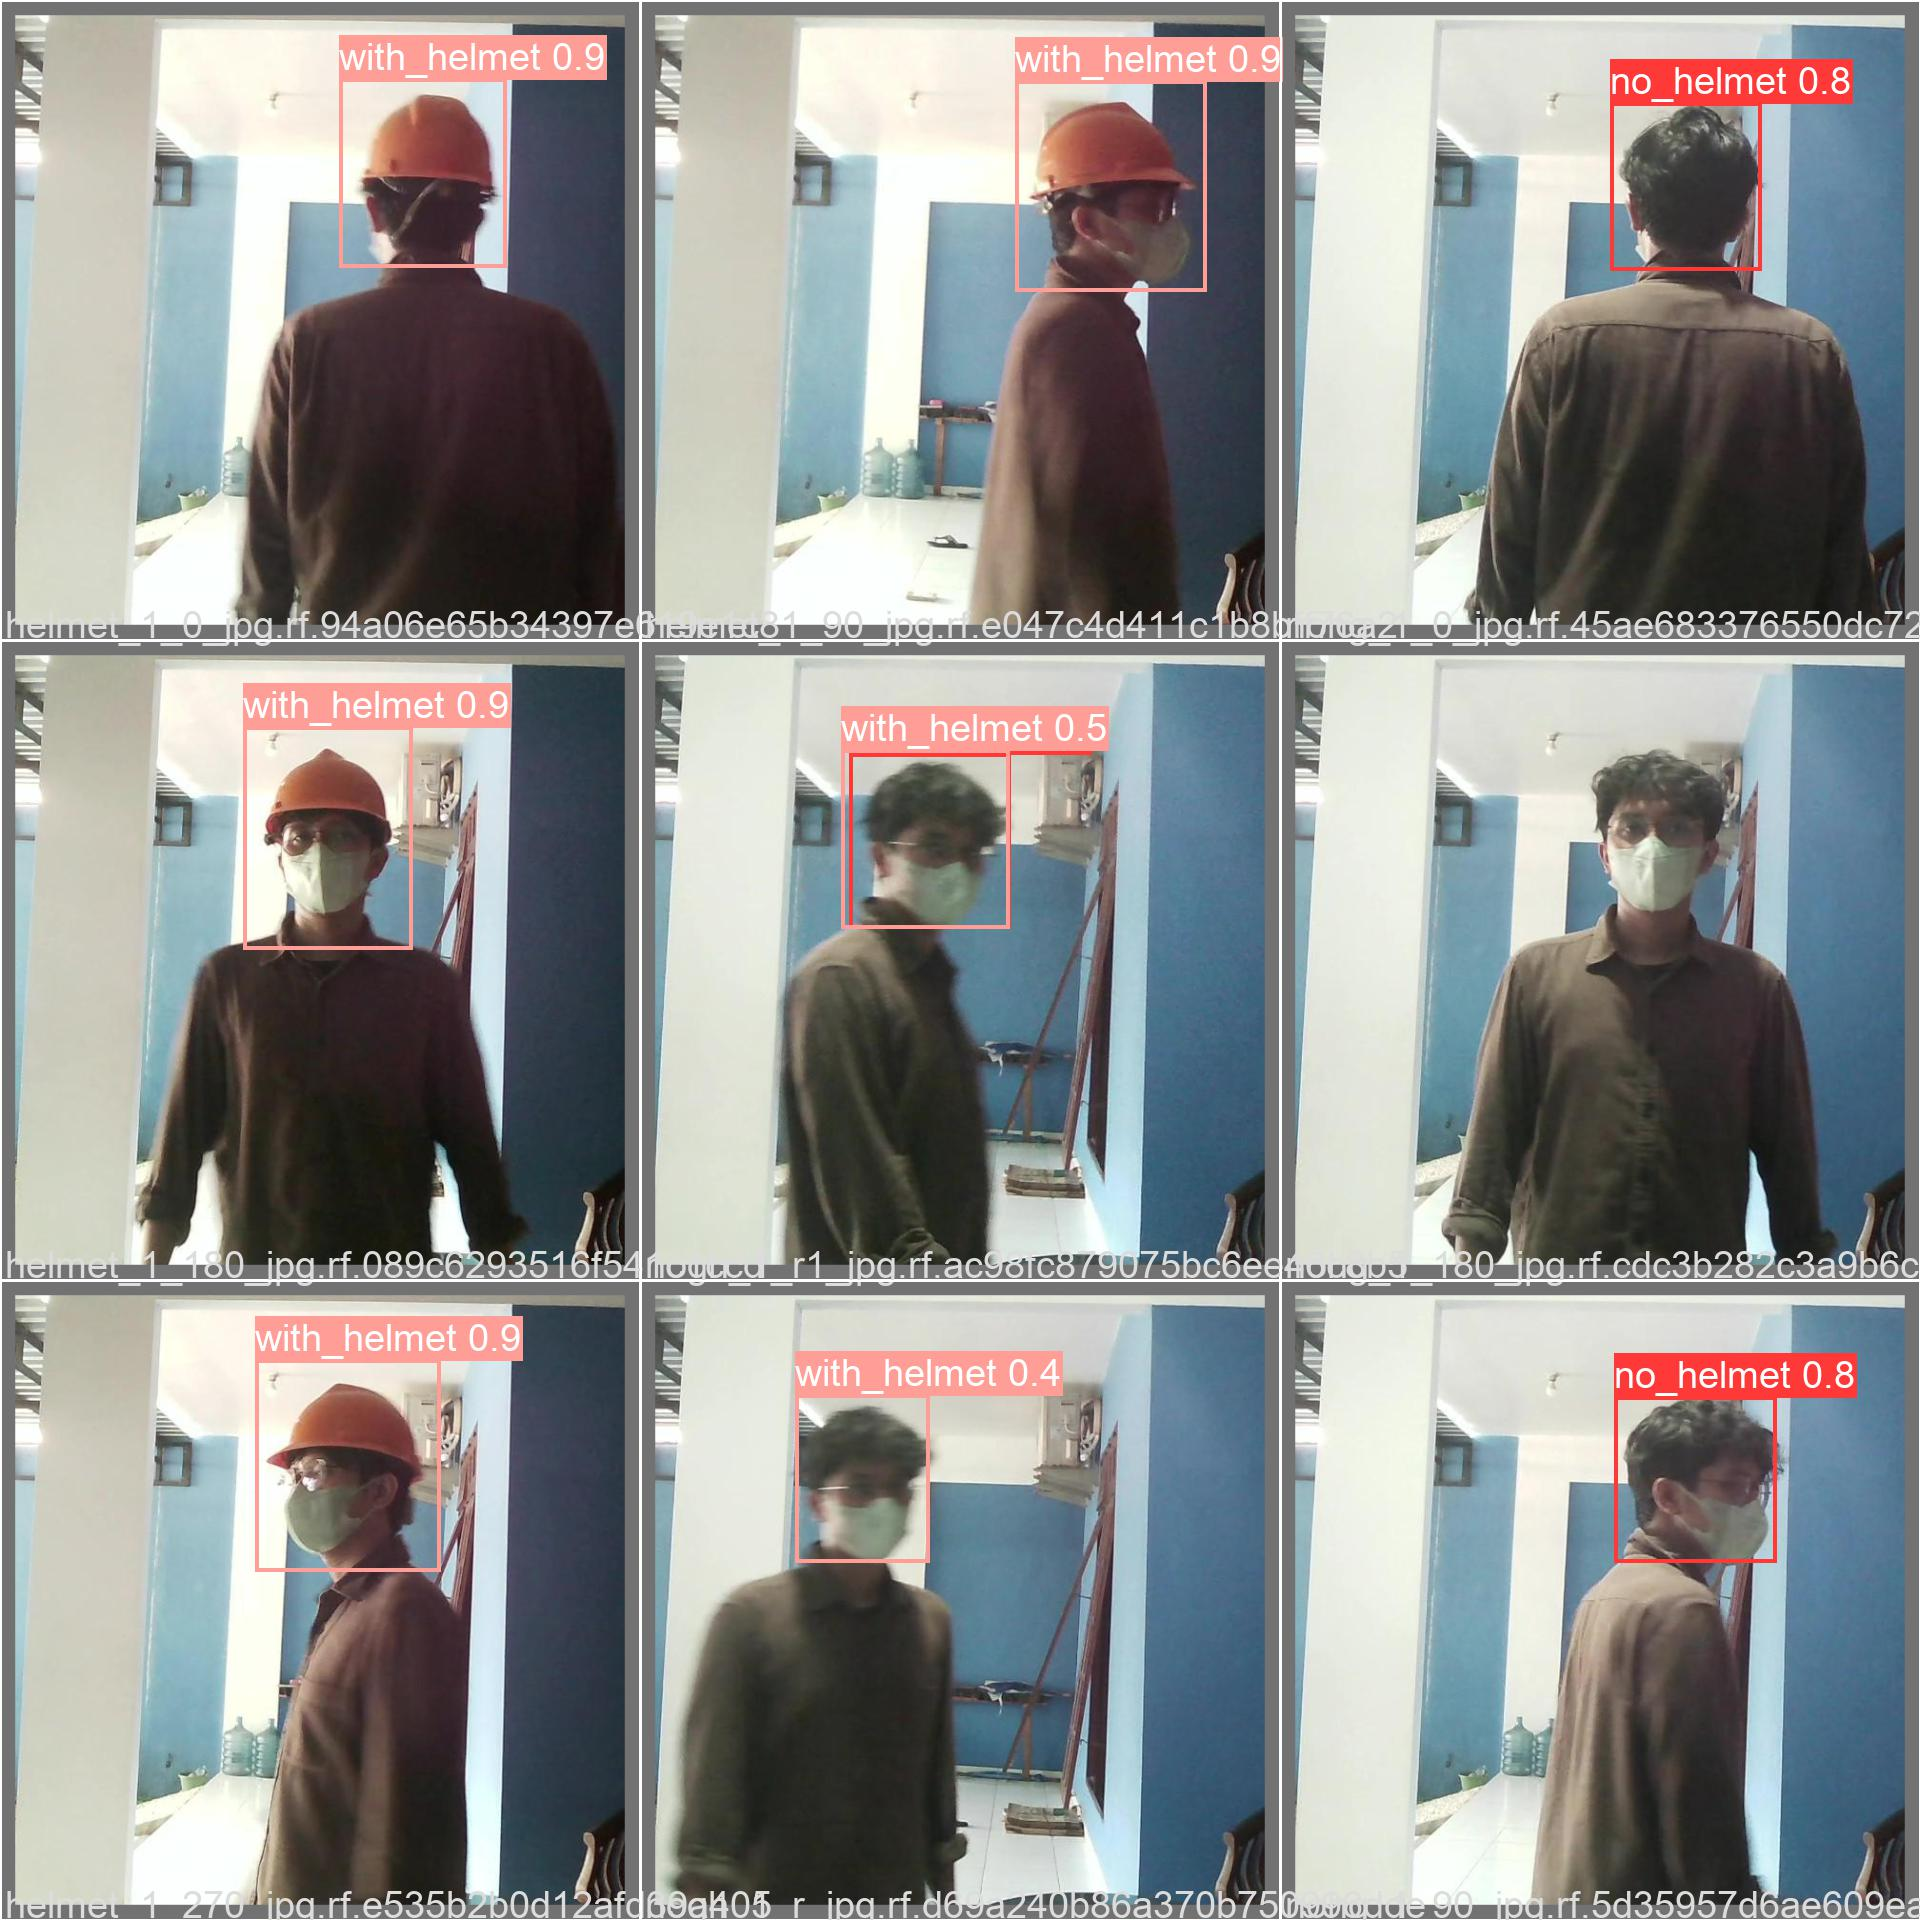
\includegraphics[width=0.31\textwidth]{gambar/BerdasarkanJarak_v2/val_hedec_pretrain_N/Jarak1_3/val_batch0_pred.jpg}
    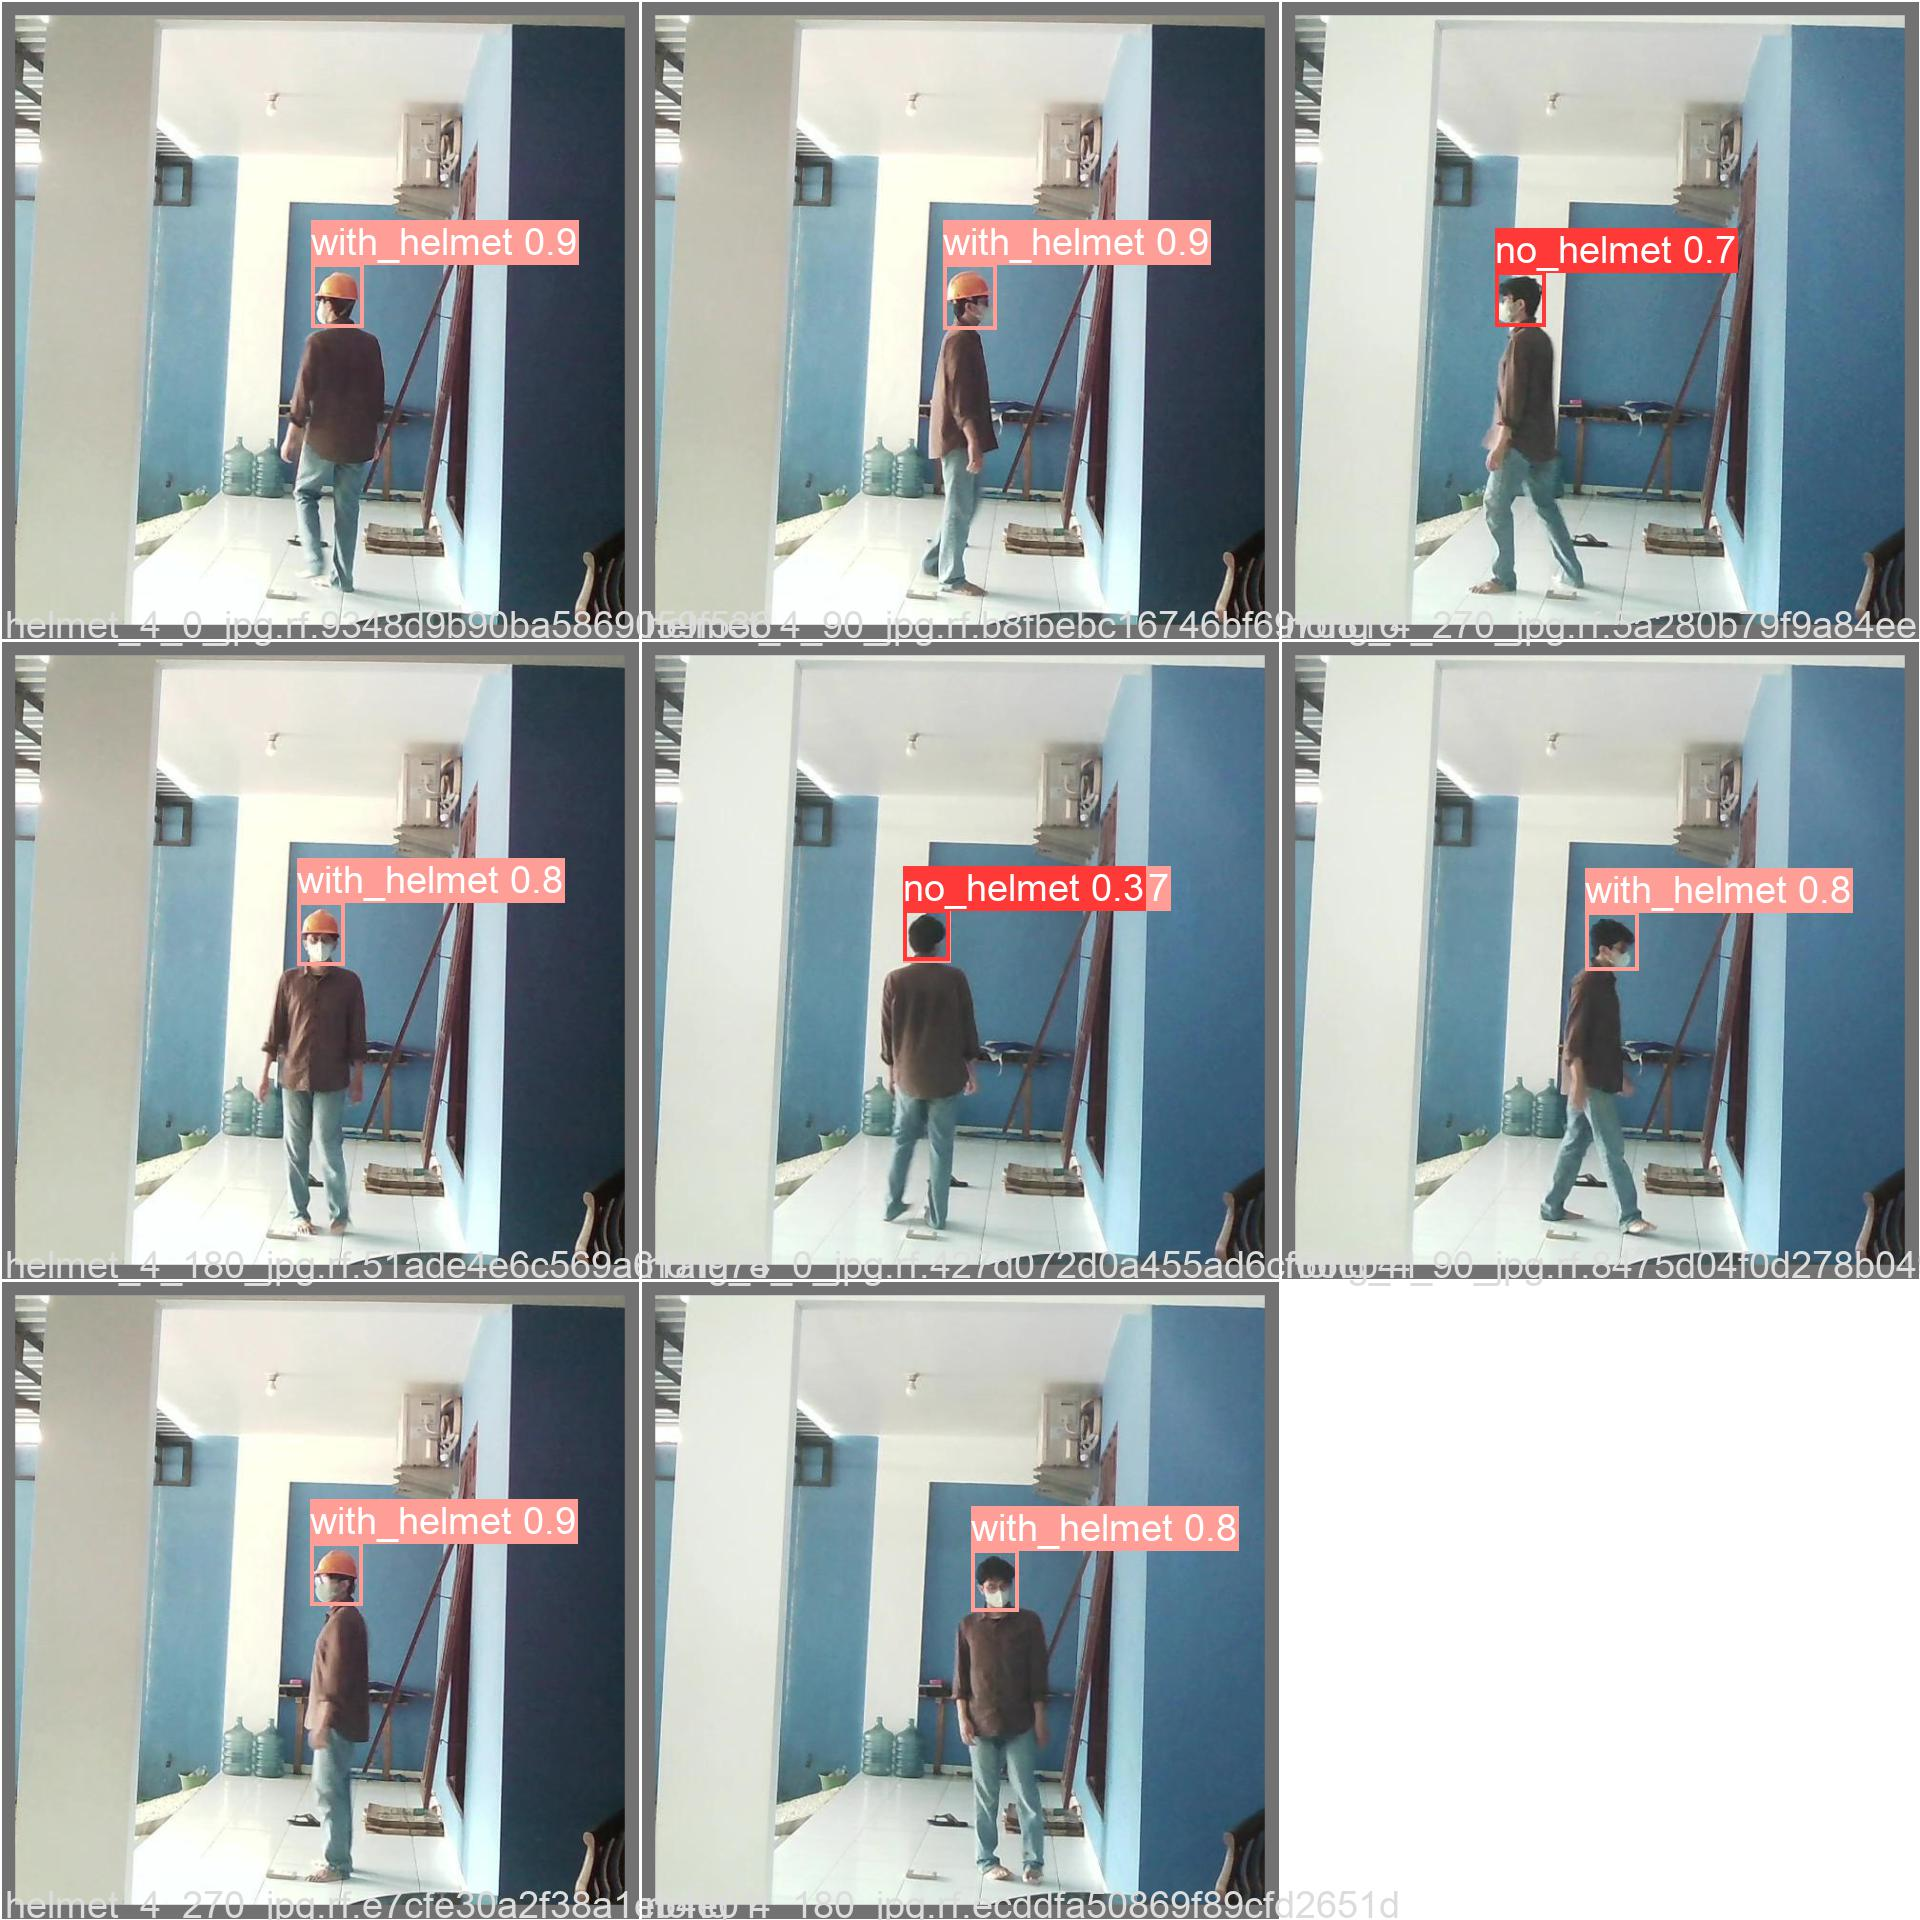
\includegraphics[width=0.31\textwidth]{gambar/BerdasarkanJarak_v2/val_hedec_pretrain_N/Jarak5_3/val_batch0_pred.jpg}
    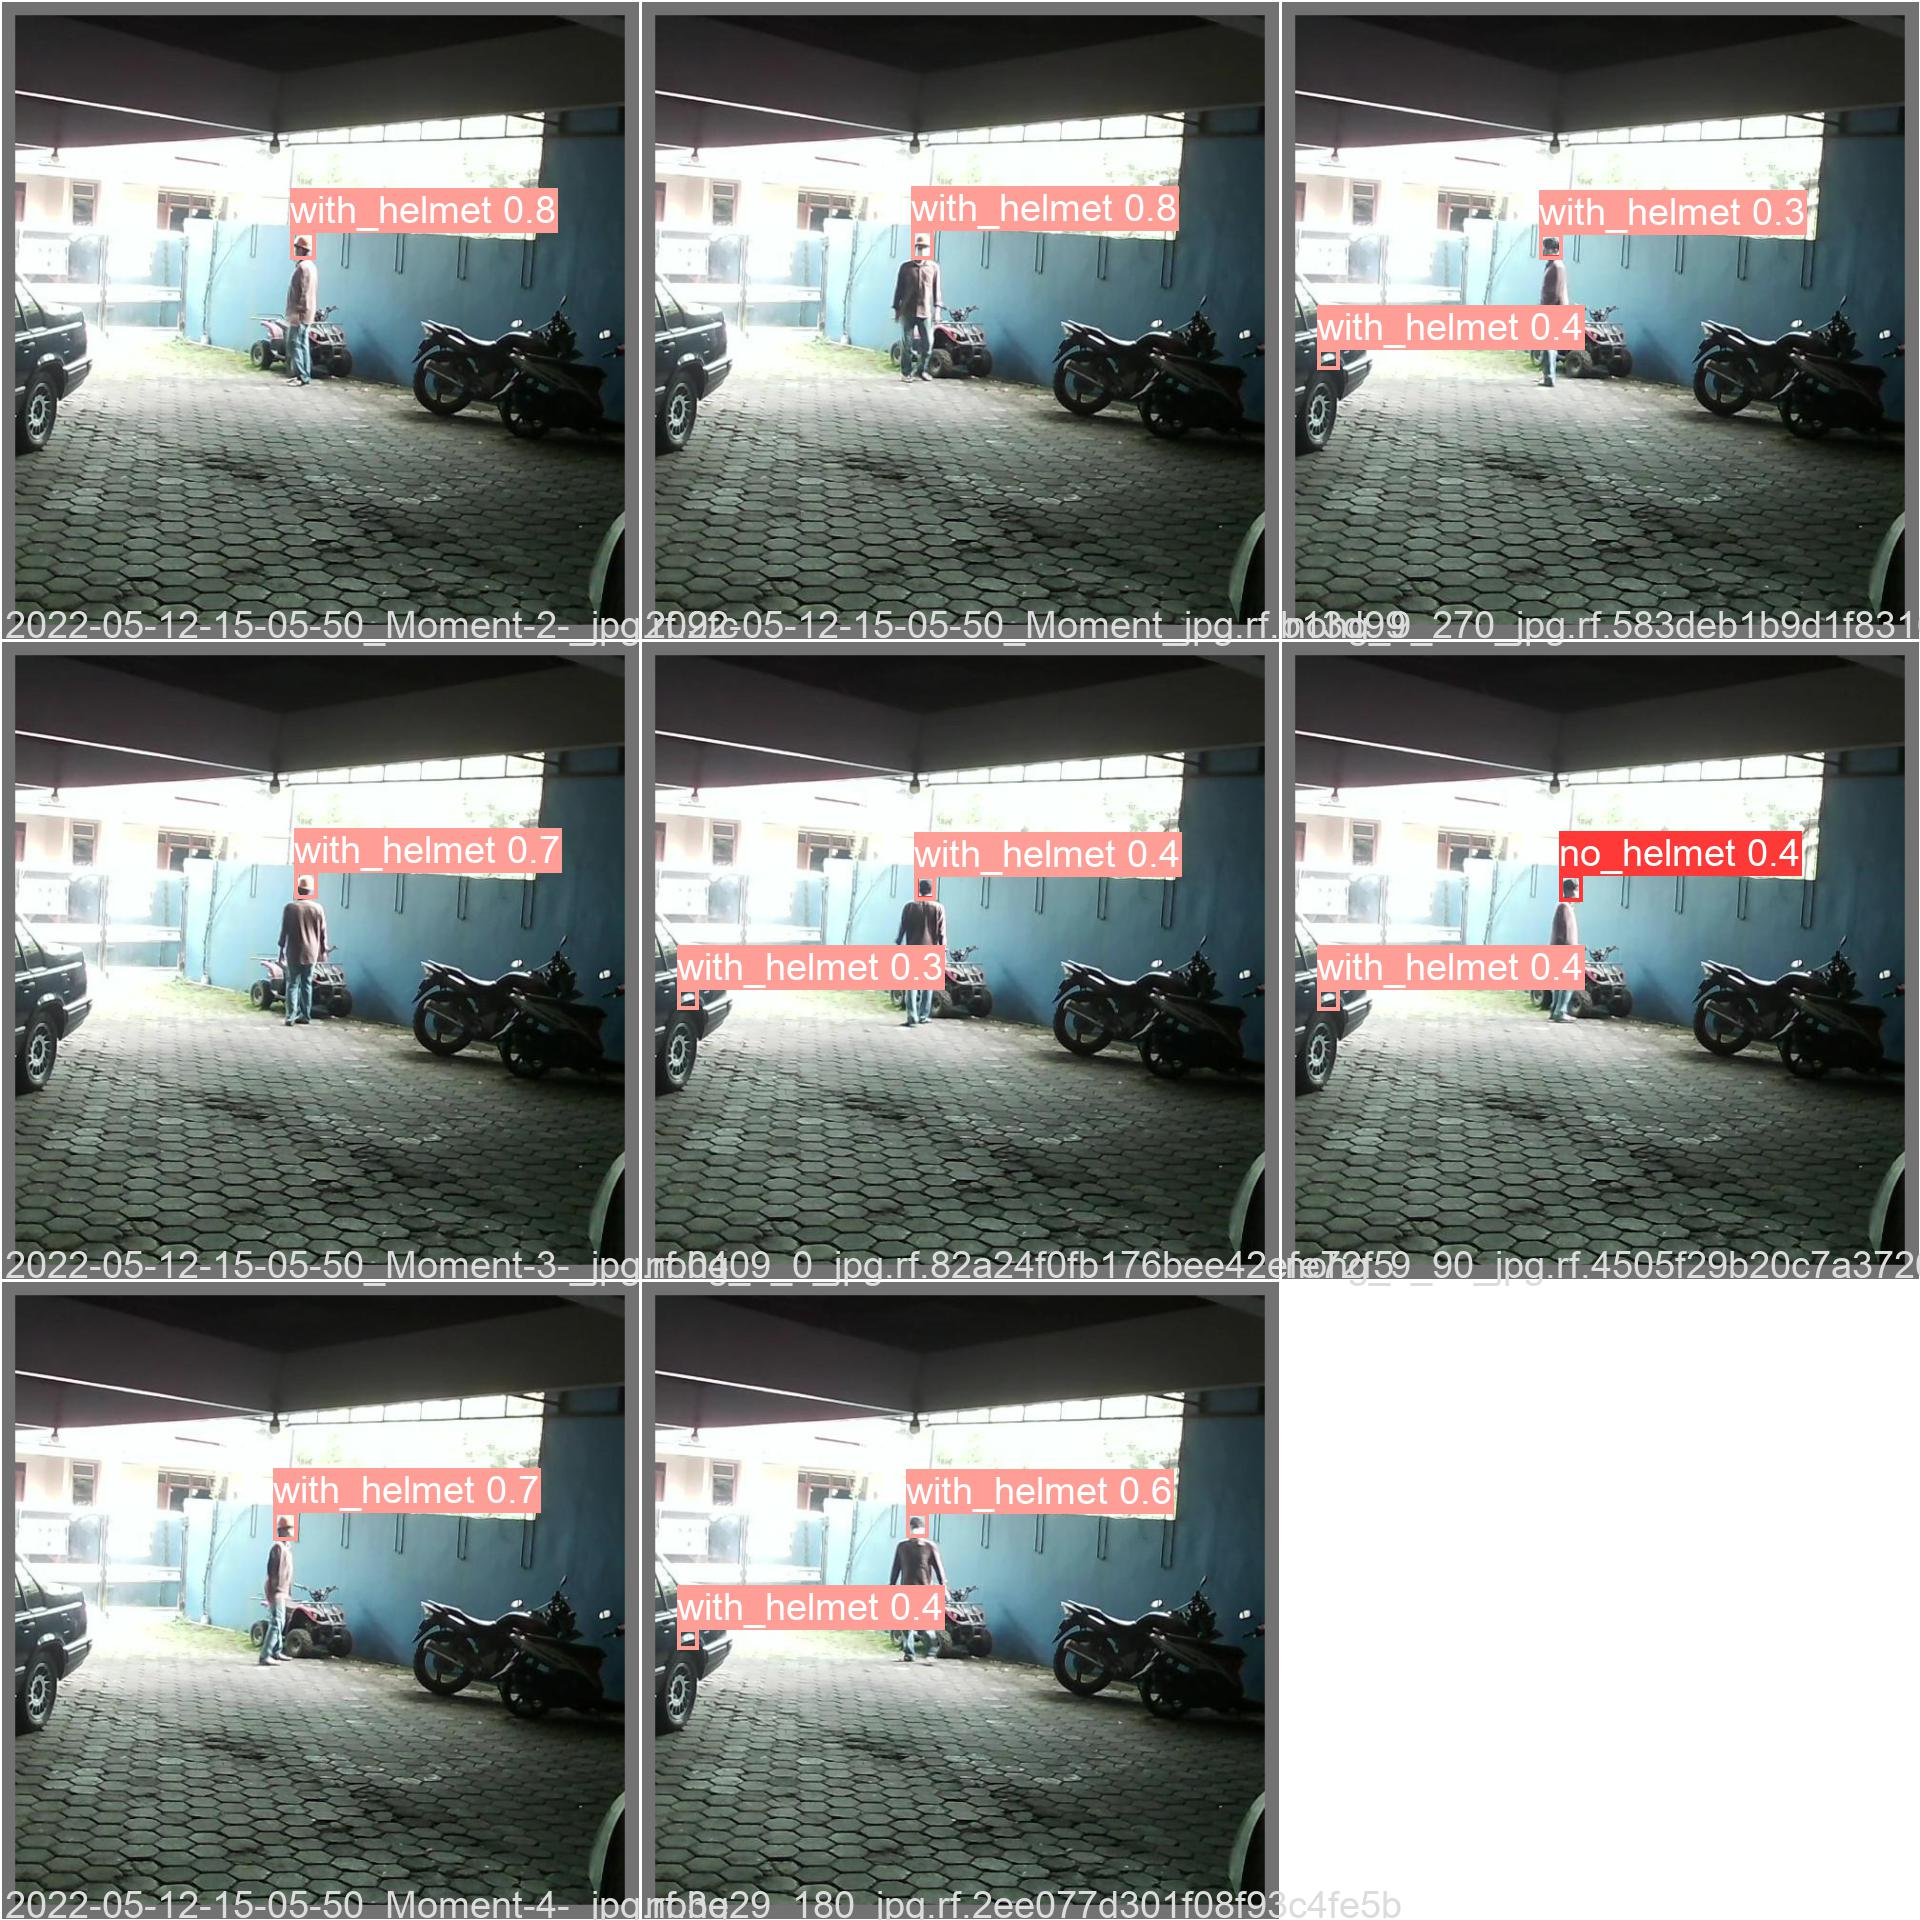
\includegraphics[width=0.31\textwidth]{gambar/BerdasarkanJarak_v2/val_hedec_pretrain_N/Jarak9/val_batch0_pred.jpg}
    \caption{Hasil Prediksi Untuk Bobot "hedec\_pretrain\_N" Pada Perbedaan Jarak}
    \label{fig:valjarak_sample_hedec_pretrain_N}  
  \end{figure}


  \item \textbf{hedec\_pretrain\_S}
  
  \par Pada pengujian jarak menggunakan bobot "hedec\_pretrain\_S", didapati bahwa bobot ini memiliki nilai metrik
  yang lebih baik daripada "hedec\_pretrain\_M". Nilai \emph{precision} rata-rata semua kelas paling rendah berada pada jarak 1.3 meter karena
  nilai \emph{precision} untuk kelas "with\_helmet" berada pada angka 0.686 dan \emph{recall} untuk kelas "no\_helmet" 0.8 karena ada beberapa 
  kelas "no\_helmet" yang salah terdeteksi sebagai "with\_helmet".

  \newpage
  \begin{longtable}{|l|l|l|l|l|} 
    \caption{Hasil Validasi Perbedaan Jarak Pada \textbf{"hedec\_pretrain\_S"}}
    \label{tb:hasiljarak_hedec_pretrain_S}\\
    \hline
    Jarak     & class        & precision & recall & mAP    \\ 
    \hline
    1.3 meter & all          & 0.843     & 0.907  & 0.995  \\
    2.6 meter & all          & 0.985     & 1      & 0.995  \\
    4 meter   & all          & 0.973     & 1      & 0.995  \\
    5.3 meter & all          & 0.986     & 1      & 0.995  \\
    6.7 meter & all          & 0.981     & 1      & 0.995  \\
    9 meter   & all          & 0.957     & 1      & 0.995  \\
    1.3 meter & no\_helmet   & 1         & 0.815  & 0.995  \\
    2.6 meter & no\_helmet   & 0.989     & 1      & 0.995  \\
    4 meter   & no\_helmet   & 0.988     & 1      & 0.995  \\
    5.3 meter & no\_helmet   & 0.988     & 1      & 0.995  \\
    6.7 meter & no\_helmet   & 0.988     & 1      & 0.995  \\
    9 meter   & no\_helmet   & 0.998     & 1      & 0.995  \\
    1.3 meter & with\_helmet & 0.686     & 1      & 0.995  \\
    2.6 meter & with\_helmet & 0.981     & 1      & 0.995  \\
    4 meter   & with\_helmet & 0.958     & 1      & 0.995  \\
    5.3 meter & with\_helmet & 0.984     & 1      & 0.995  \\
    6.7 meter & with\_helmet & 0.974     & 1      & 0.995  \\
    9 meter   & with\_helmet & 0.916     & 1      & 0.995  \\
    \hline
  \end{longtable}

  \begin{figure}[h!]
    \centering
    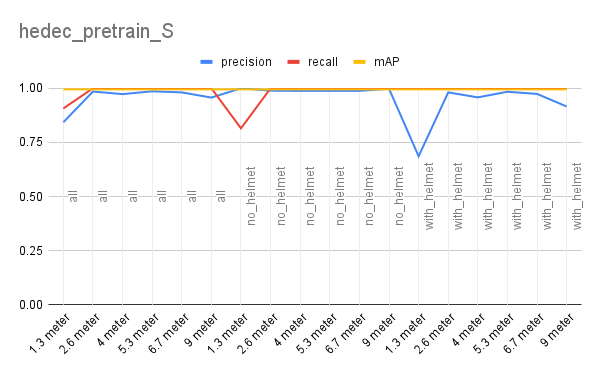
\includegraphics[width=1\textwidth]{gambar/BerdasarkanJarak/hedec_pretrain_S.png}
    \caption{Grafik \emph{Precision, Recall, mAP} untuk \textbf{"hedec\_pretrain\_S"} Pada Jarak 1.3 meter Hingga 9 meter}
    \label{fig:grafvaljarak_hedec_pretrain_S}  
  \end{figure}

  \begin{figure} [h!]
    \centering
    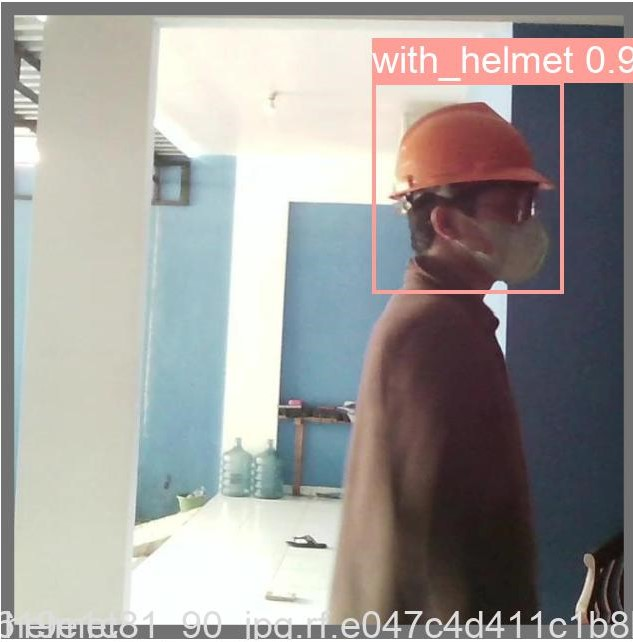
\includegraphics[width=0.31\textwidth]{gambar/BerdasarkanJarak_v2/val_hedec_pretrain_S/Jarak1_3/val_batch0_pred.jpg}
    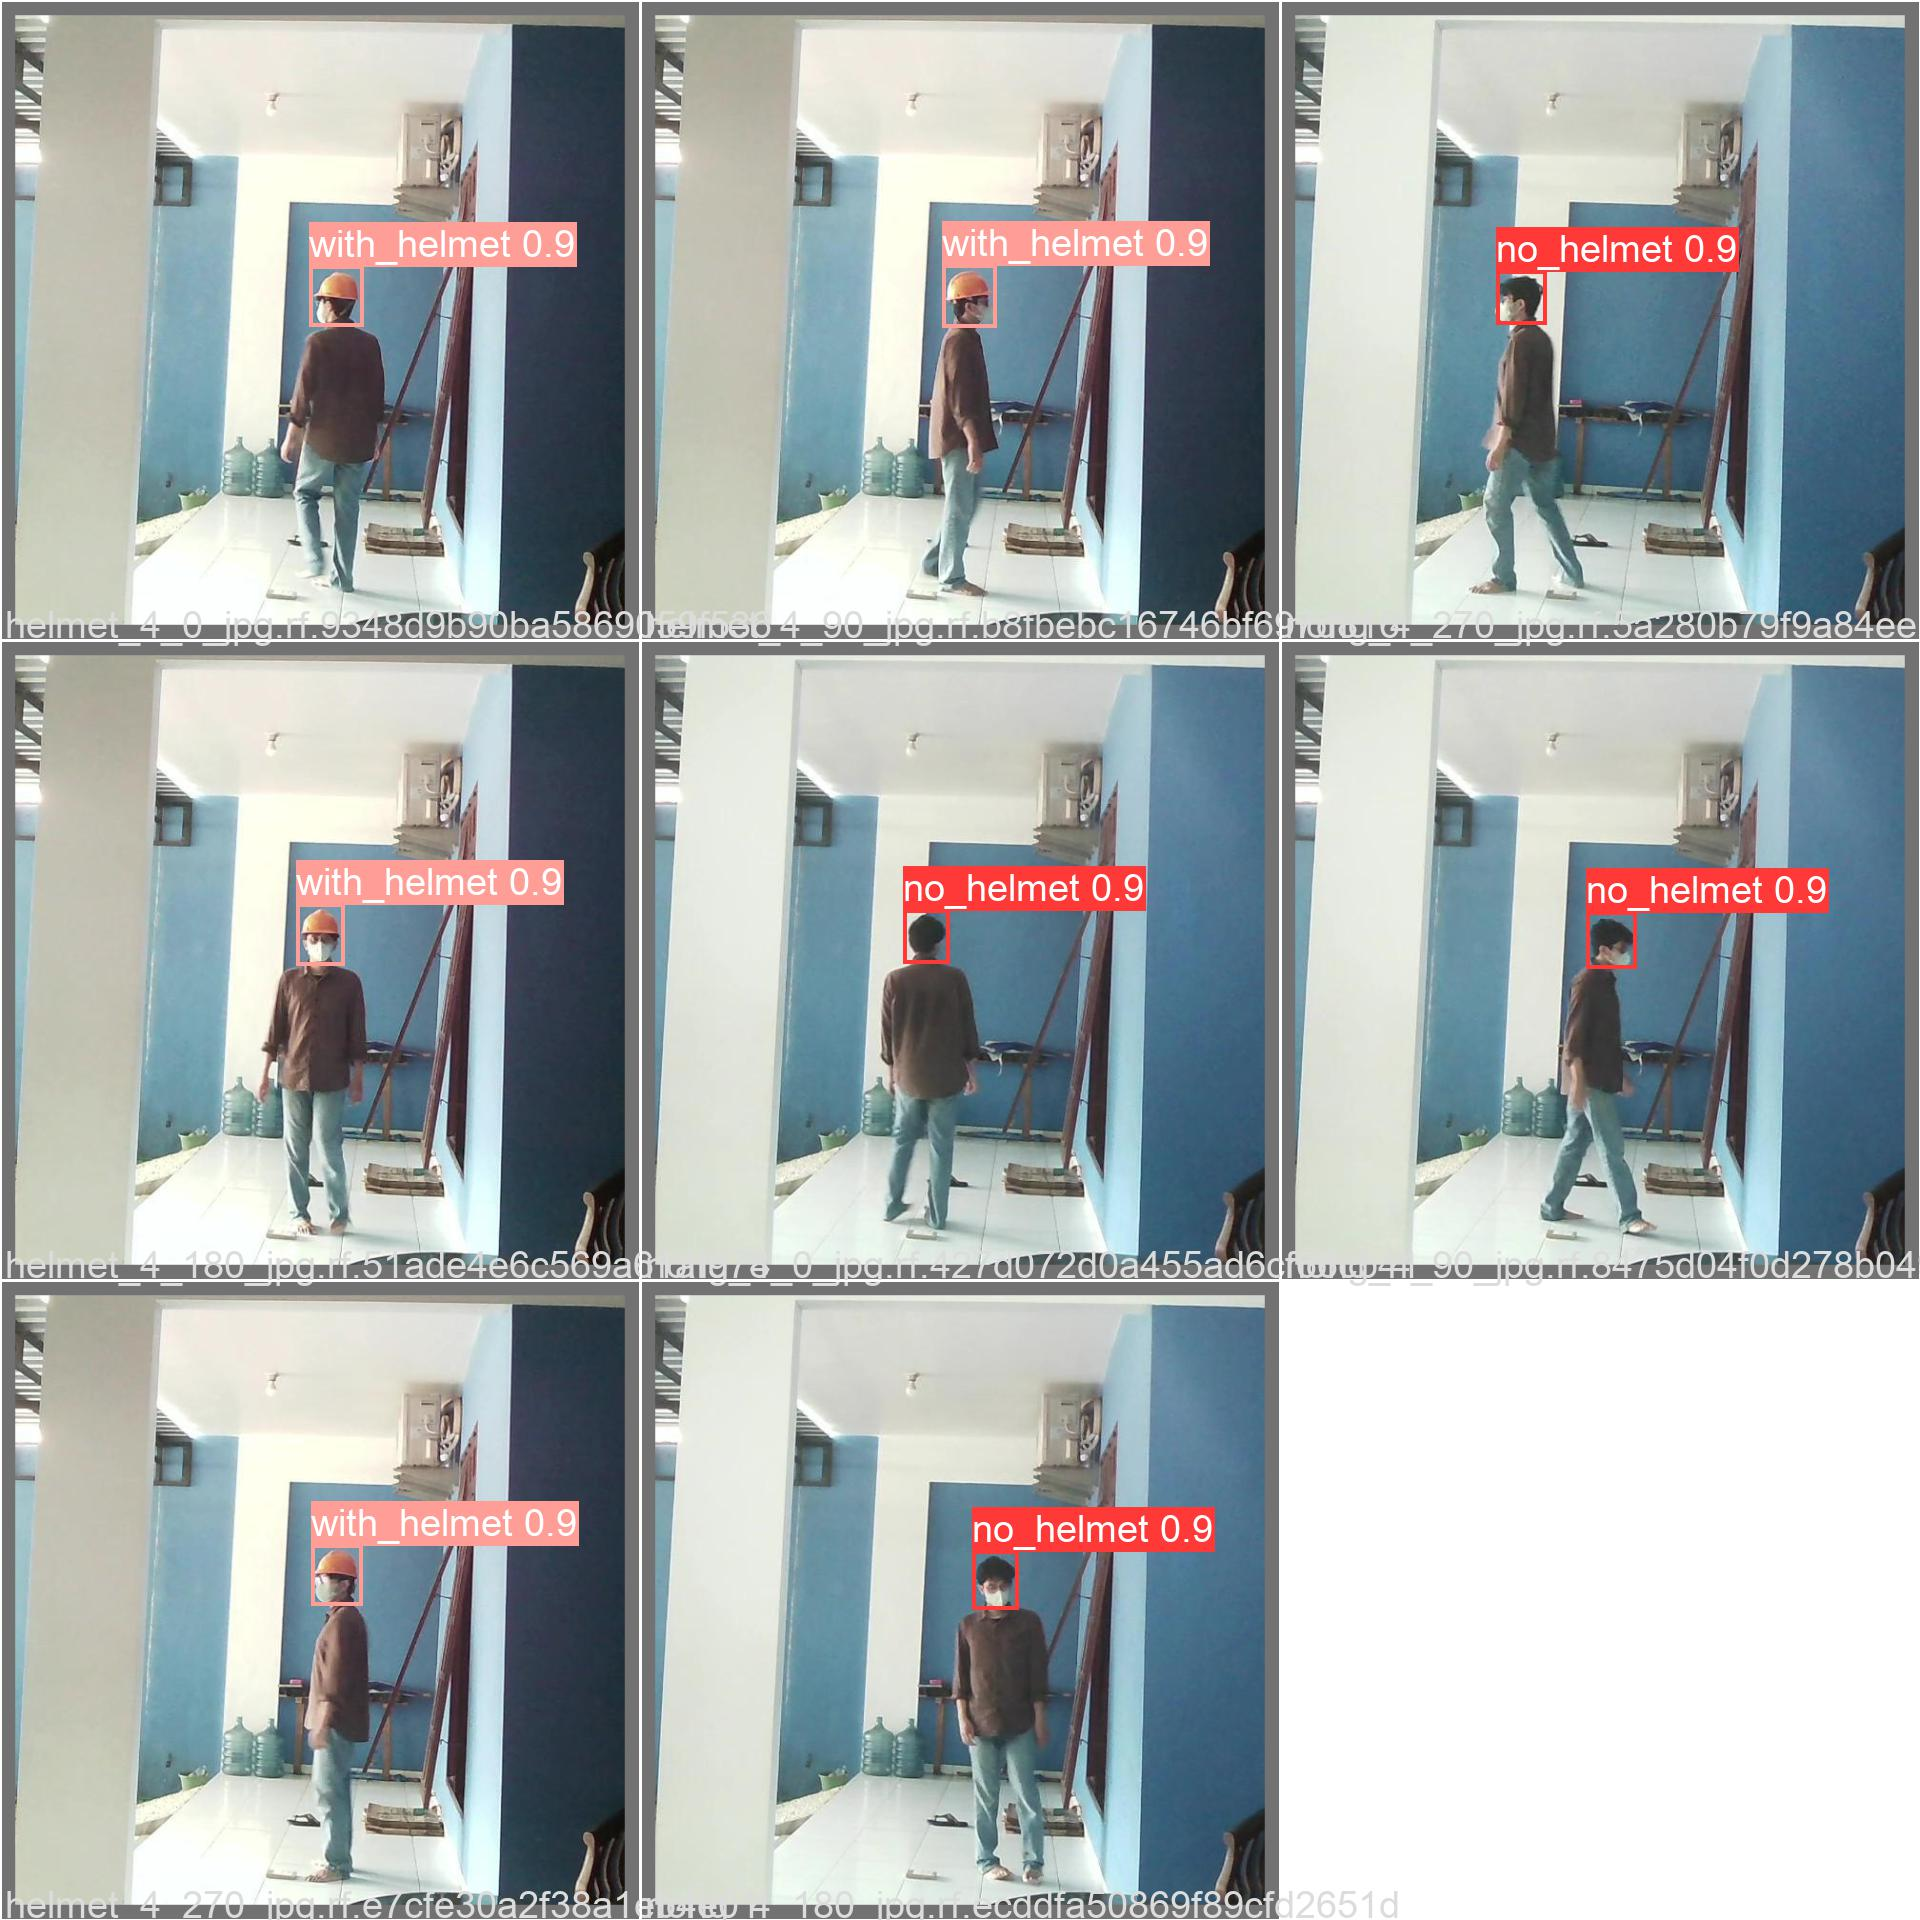
\includegraphics[width=0.31\textwidth]{gambar/BerdasarkanJarak_v2/val_hedec_pretrain_S/Jarak5_3/val_batch0_pred.jpg}
    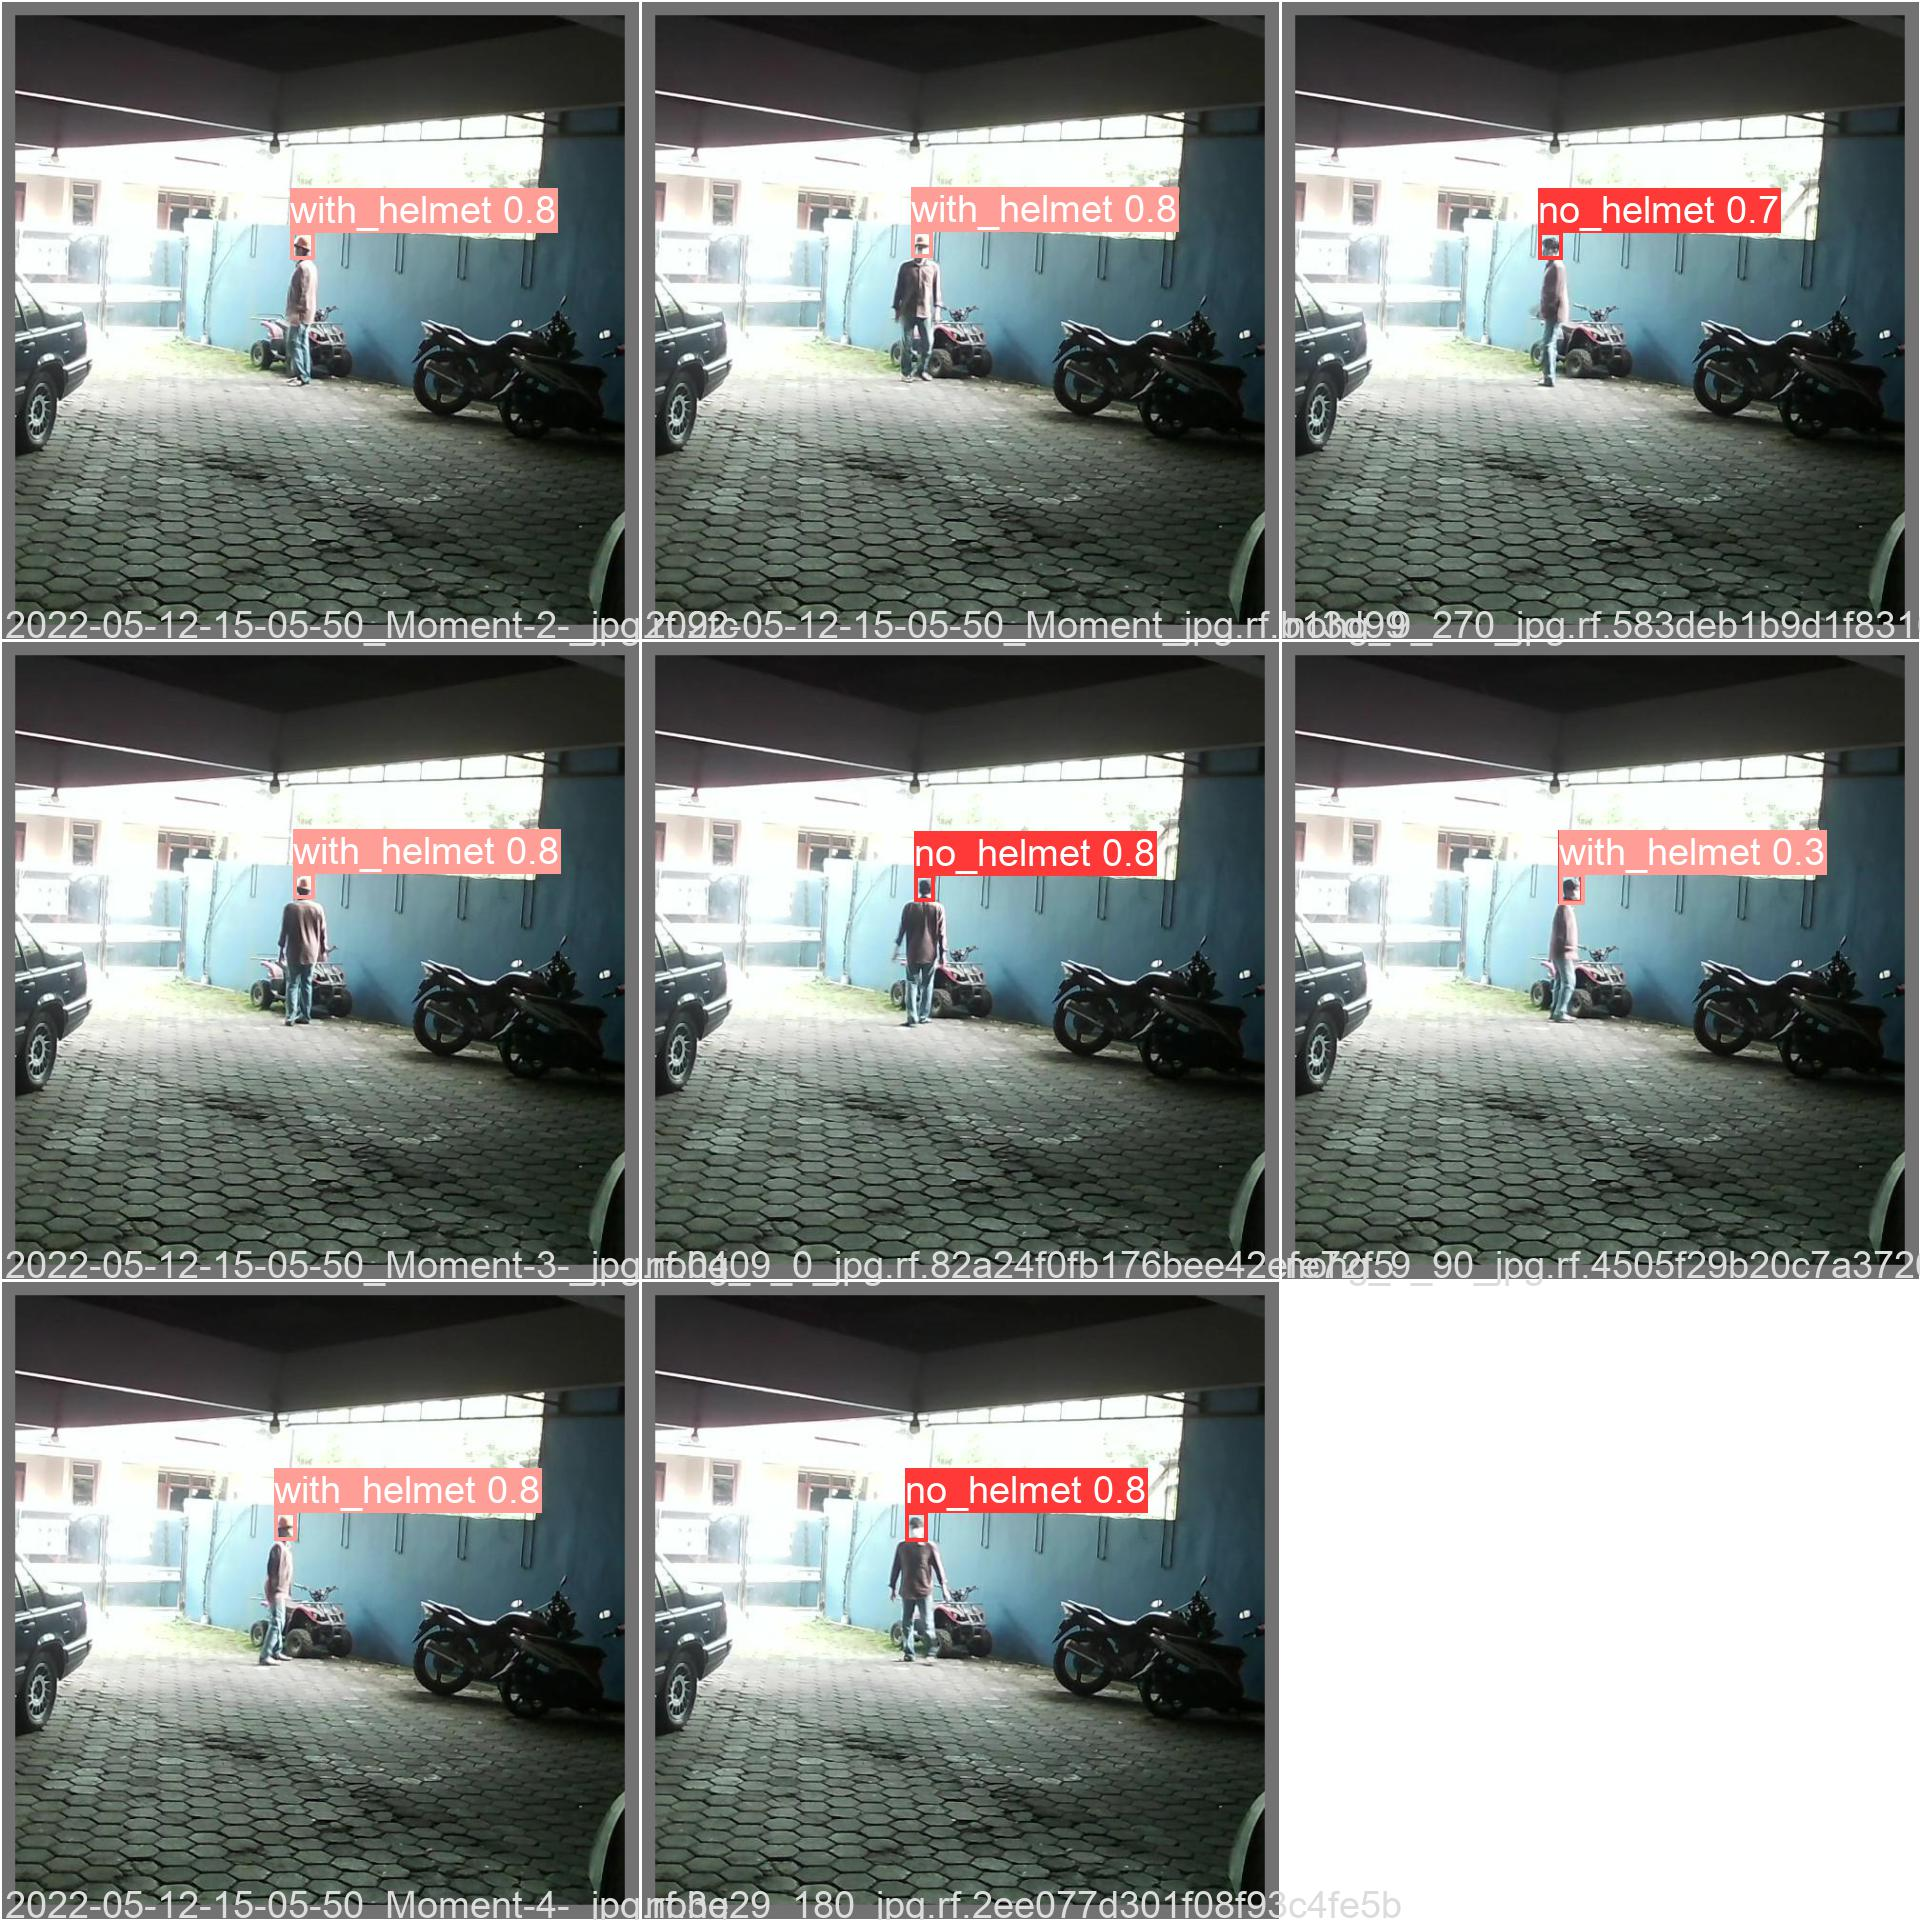
\includegraphics[width=0.31\textwidth]{gambar/BerdasarkanJarak_v2/val_hedec_pretrain_S/Jarak9/val_batch0_pred.jpg}
    \caption{Hasil Prediksi Untuk Bobot "hedec\_pretrain\_S" Pada Perbedaan Jarak}
    \label{fig:valjarak_sample_hedec_pretrain_S}  
  \end{figure}

  \FloatBarrier
  
   
  \item \textbf{hedec\_pretrain\_M}
  
  \par Pada pengujian menggunakan bobot "hedec\_pretrain\_M" pada perbedaan jarak seperti yang bisa dilihat di Gambar~\ref{fig:grafvaljarak_hedec_pretrain_M}, jarak 1.3 meter dan 9 meter
  secara umum memiliki nilai yang sangat buruk. Pada jarak 1.3 meter, nilai \emph{precision} untuk kelas "with\_helmet"
  mencapai nilai 0.374 sedangkan pada jarak 9 meter mendapatkan nilai 0.26. Untuk kelas "no\_helmet" untuk semua jarak memiliki
  nilai yang bagus diatas 0.9 untuk presisinya. Terlihat untuk \emph{weight} ini mengalami kesulitan untuk mendeteksi
  kelas "with\_helmet" pada jarak 1.3 meter dan pada jarak 9 meter.


  \begin{longtable}{|l|l|l|l|l|} 
    \caption{Hasil Validasi Perbedaan Jarak Pada \textbf{"hedec\_pretrain\_M"}}
    \label{tb:hasiljarak_hedec_pretrain_M}\\
    \hline
    Jarak     & class        & precision & recall & mAP    \\ 
    \hline
    \endhead
    1.3 meter & all          & 0.687     & 0.827  & 0.891  \\
    2.6 meter & all          & 0.981     & 1      & 0.995  \\
    4 meter   & all          & 0.826     & 0.988  & 0.995  \\
    5.3 meter & all          & 0.874     & 0.994  & 0.995  \\
    6.7 meter & all          & 0.858     & 0.991  & 0.995  \\
    9 meter   & all          & 0.63      & 0.933  & 0.995  \\
    1.3 meter & no\_helmet   & 1         & 0.655  & 0.995  \\
    2.6 meter & no\_helmet   & 0.989     & 1      & 0.995  \\
    4 meter   & no\_helmet   & 1         & 0.976  & 0.995  \\
    5.3 meter & no\_helmet   & 1         & 0.989  & 0.995  \\
    6.7 meter & no\_helmet   & 1         & 0.983  & 0.995  \\
    9 meter   & no\_helmet   & 1         & 0.866  & 0.995  \\
    1.3 meter & with\_helmet & 0.374     & 1      & 0.787  \\
    2.6 meter & with\_helmet & 0.973     & 1      & 0.995  \\
    4 meter   & with\_helmet & 0.651     & 1      & 0.995  \\
    5.3 meter & with\_helmet & 0.747     & 1      & 0.995  \\
    6.7 meter & with\_helmet & 0.716     & 1      & 0.995  \\
    9 meter   & with\_helmet & 0.26      & 1      & 0.995  \\
    \hline
  \end{longtable}

  \begin{figure} [h!]
    \centering
    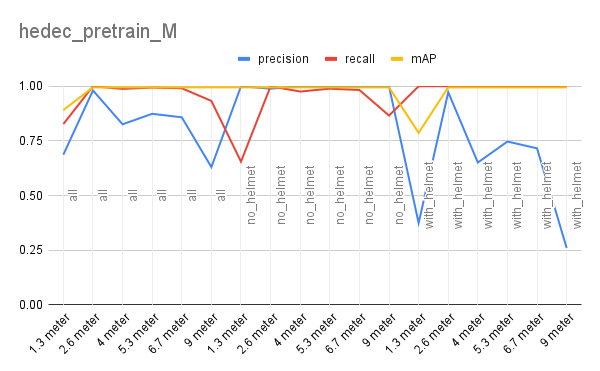
\includegraphics[width=1\textwidth]{gambar/BerdasarkanJarak/hedec_pretrain_M.png}
    \caption{Grafik \emph{Precision, Recall, mAP} untuk \textbf{"hedec\_pretrain\_M"} Pada Jarak 1.3 meter Hingga 9 meter}
    \label{fig:grafvaljarak_hedec_pretrain_M}  
  \end{figure}

  \FloatBarrier

  \begin{figure} [h!]
    \centering
    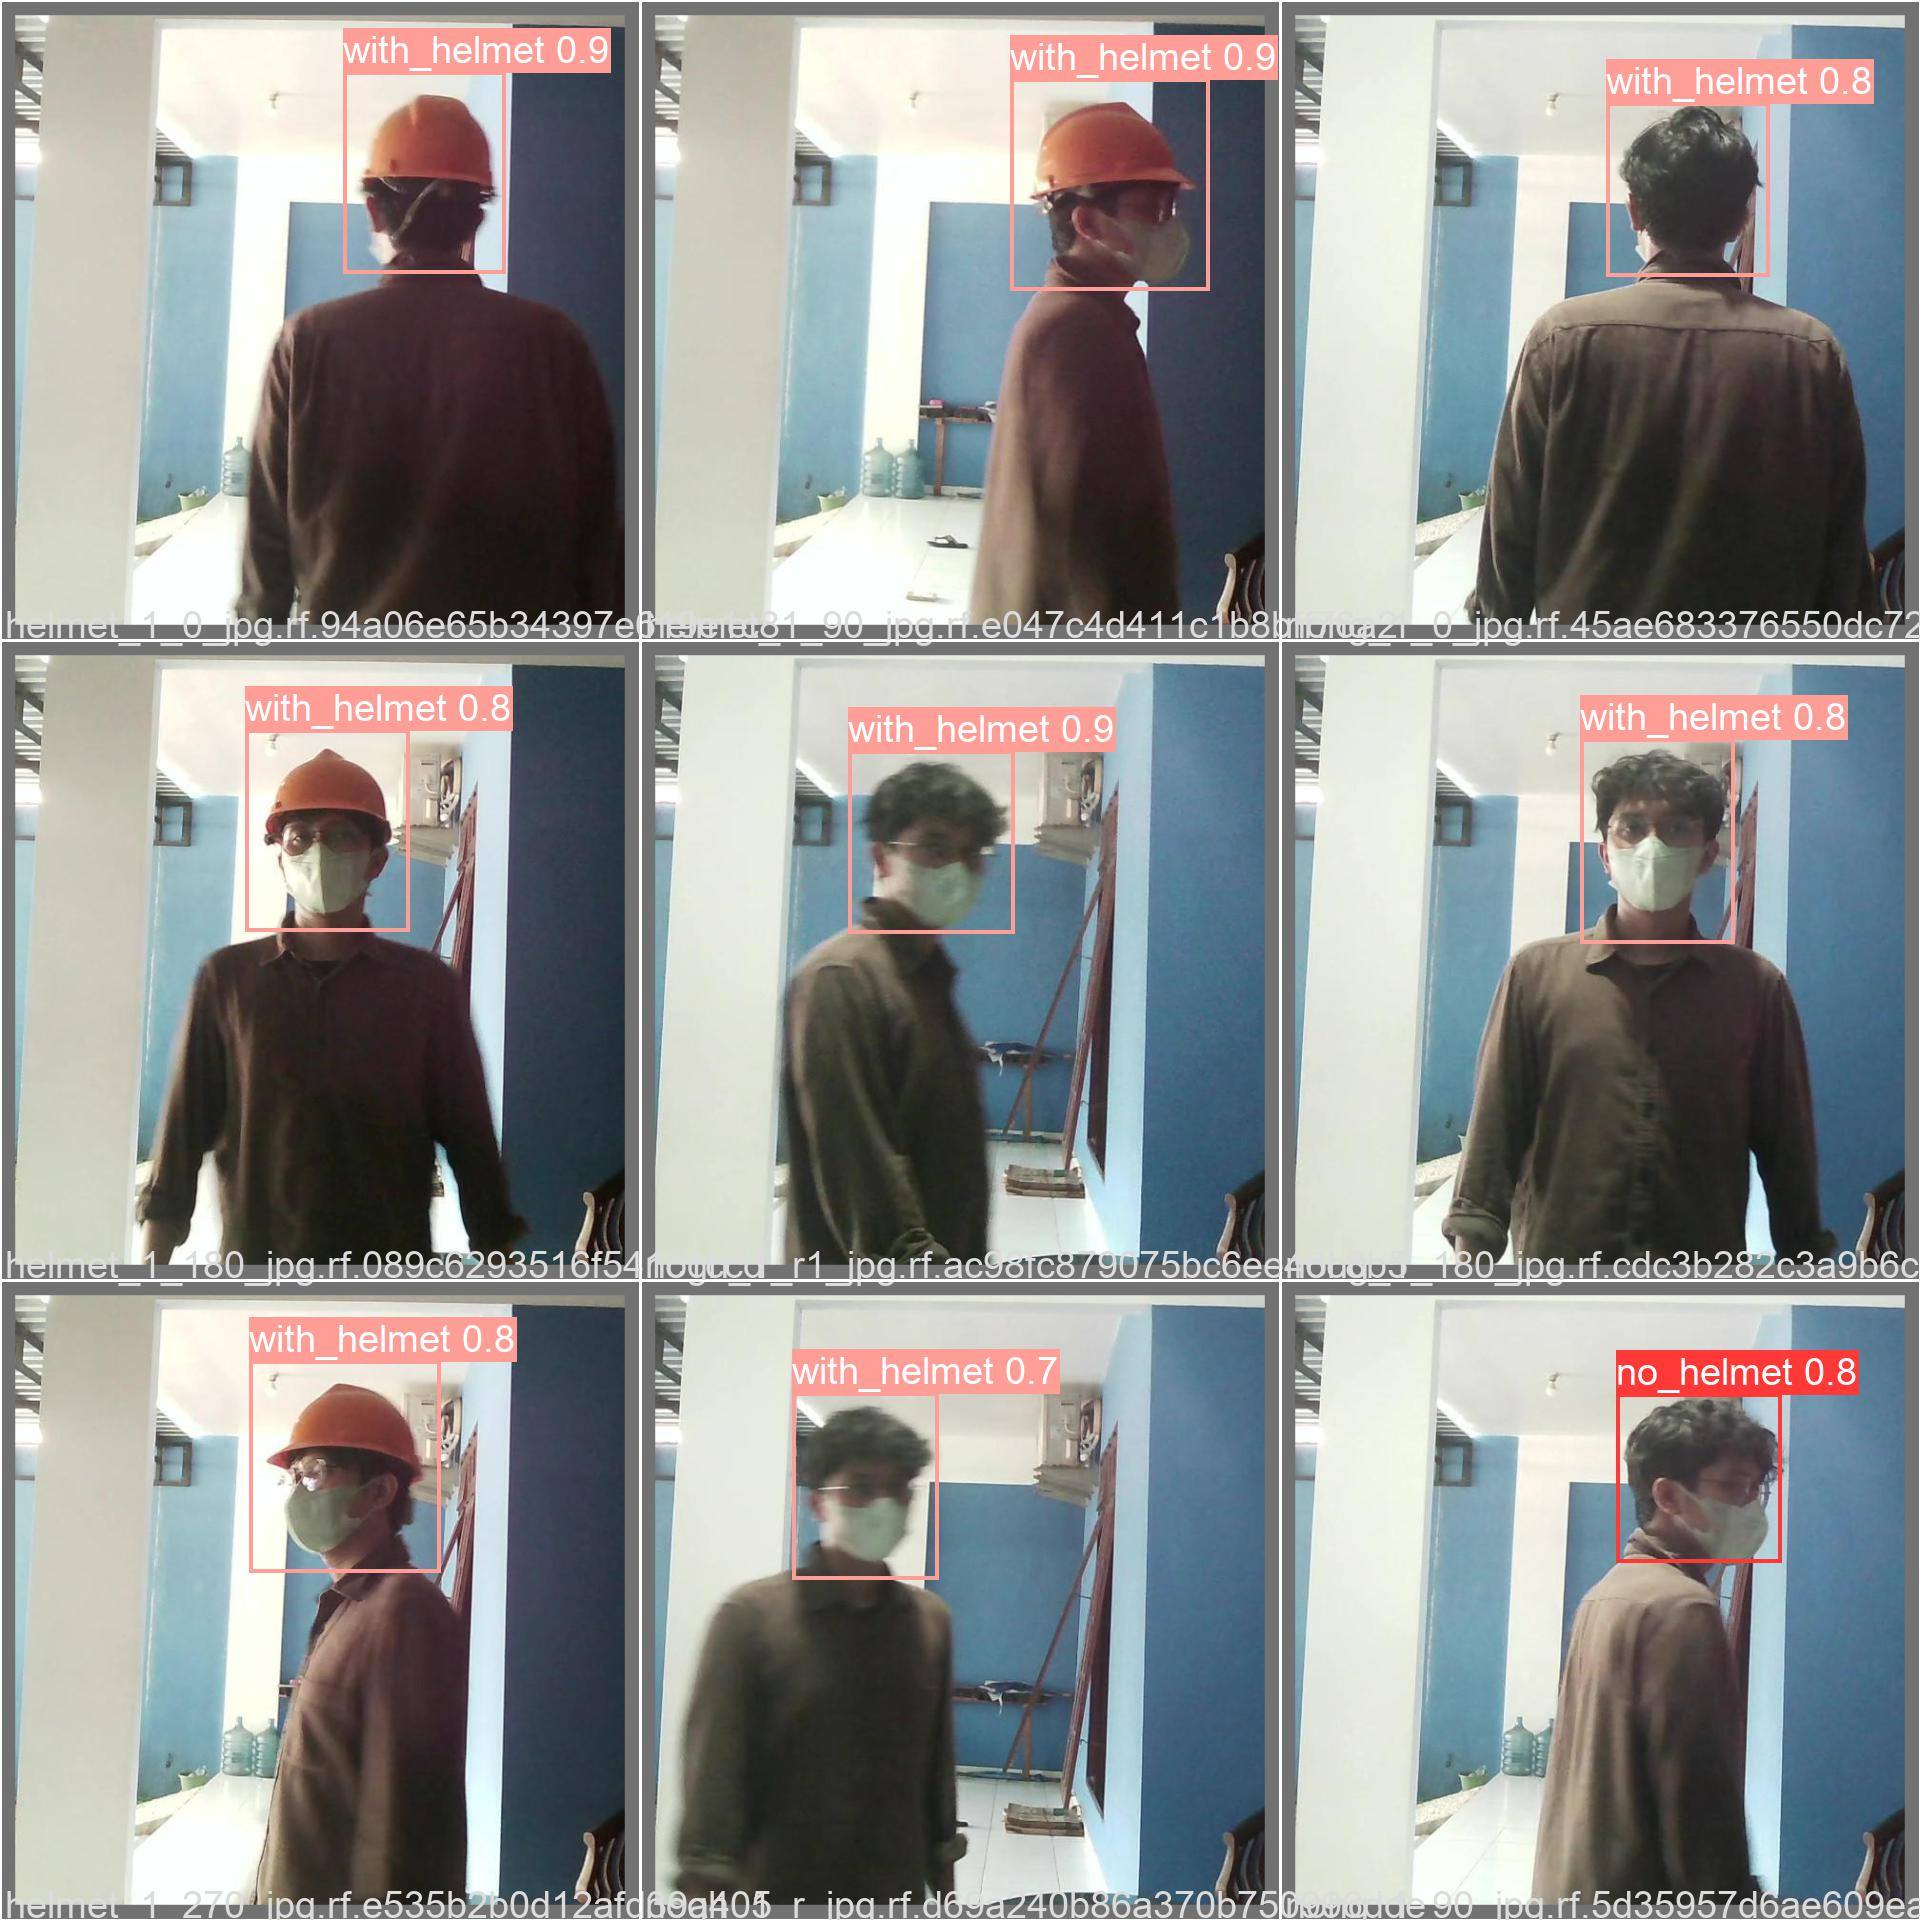
\includegraphics[width=0.31\textwidth]{gambar/BerdasarkanJarak_v2/val_hedec_pretrain_M/Jarak1_3/val_batch0_pred.jpg}
    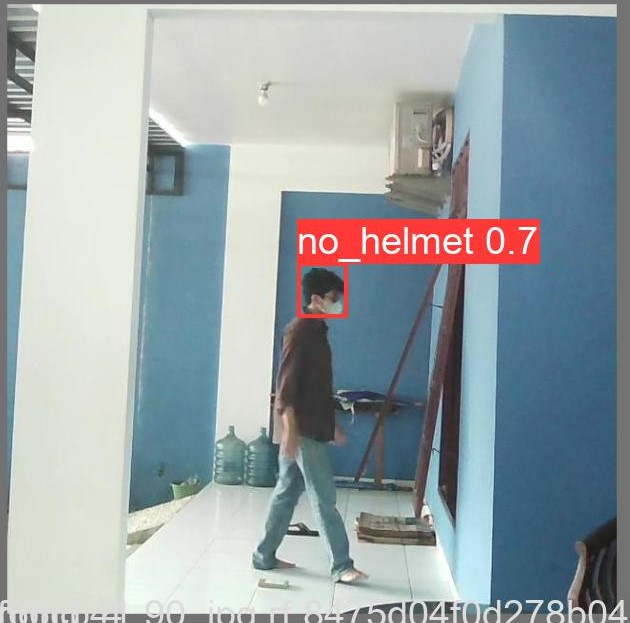
\includegraphics[width=0.31\textwidth]{gambar/BerdasarkanJarak_v2/val_hedec_pretrain_M/Jarak5_3/val_batch0_pred.jpg}
    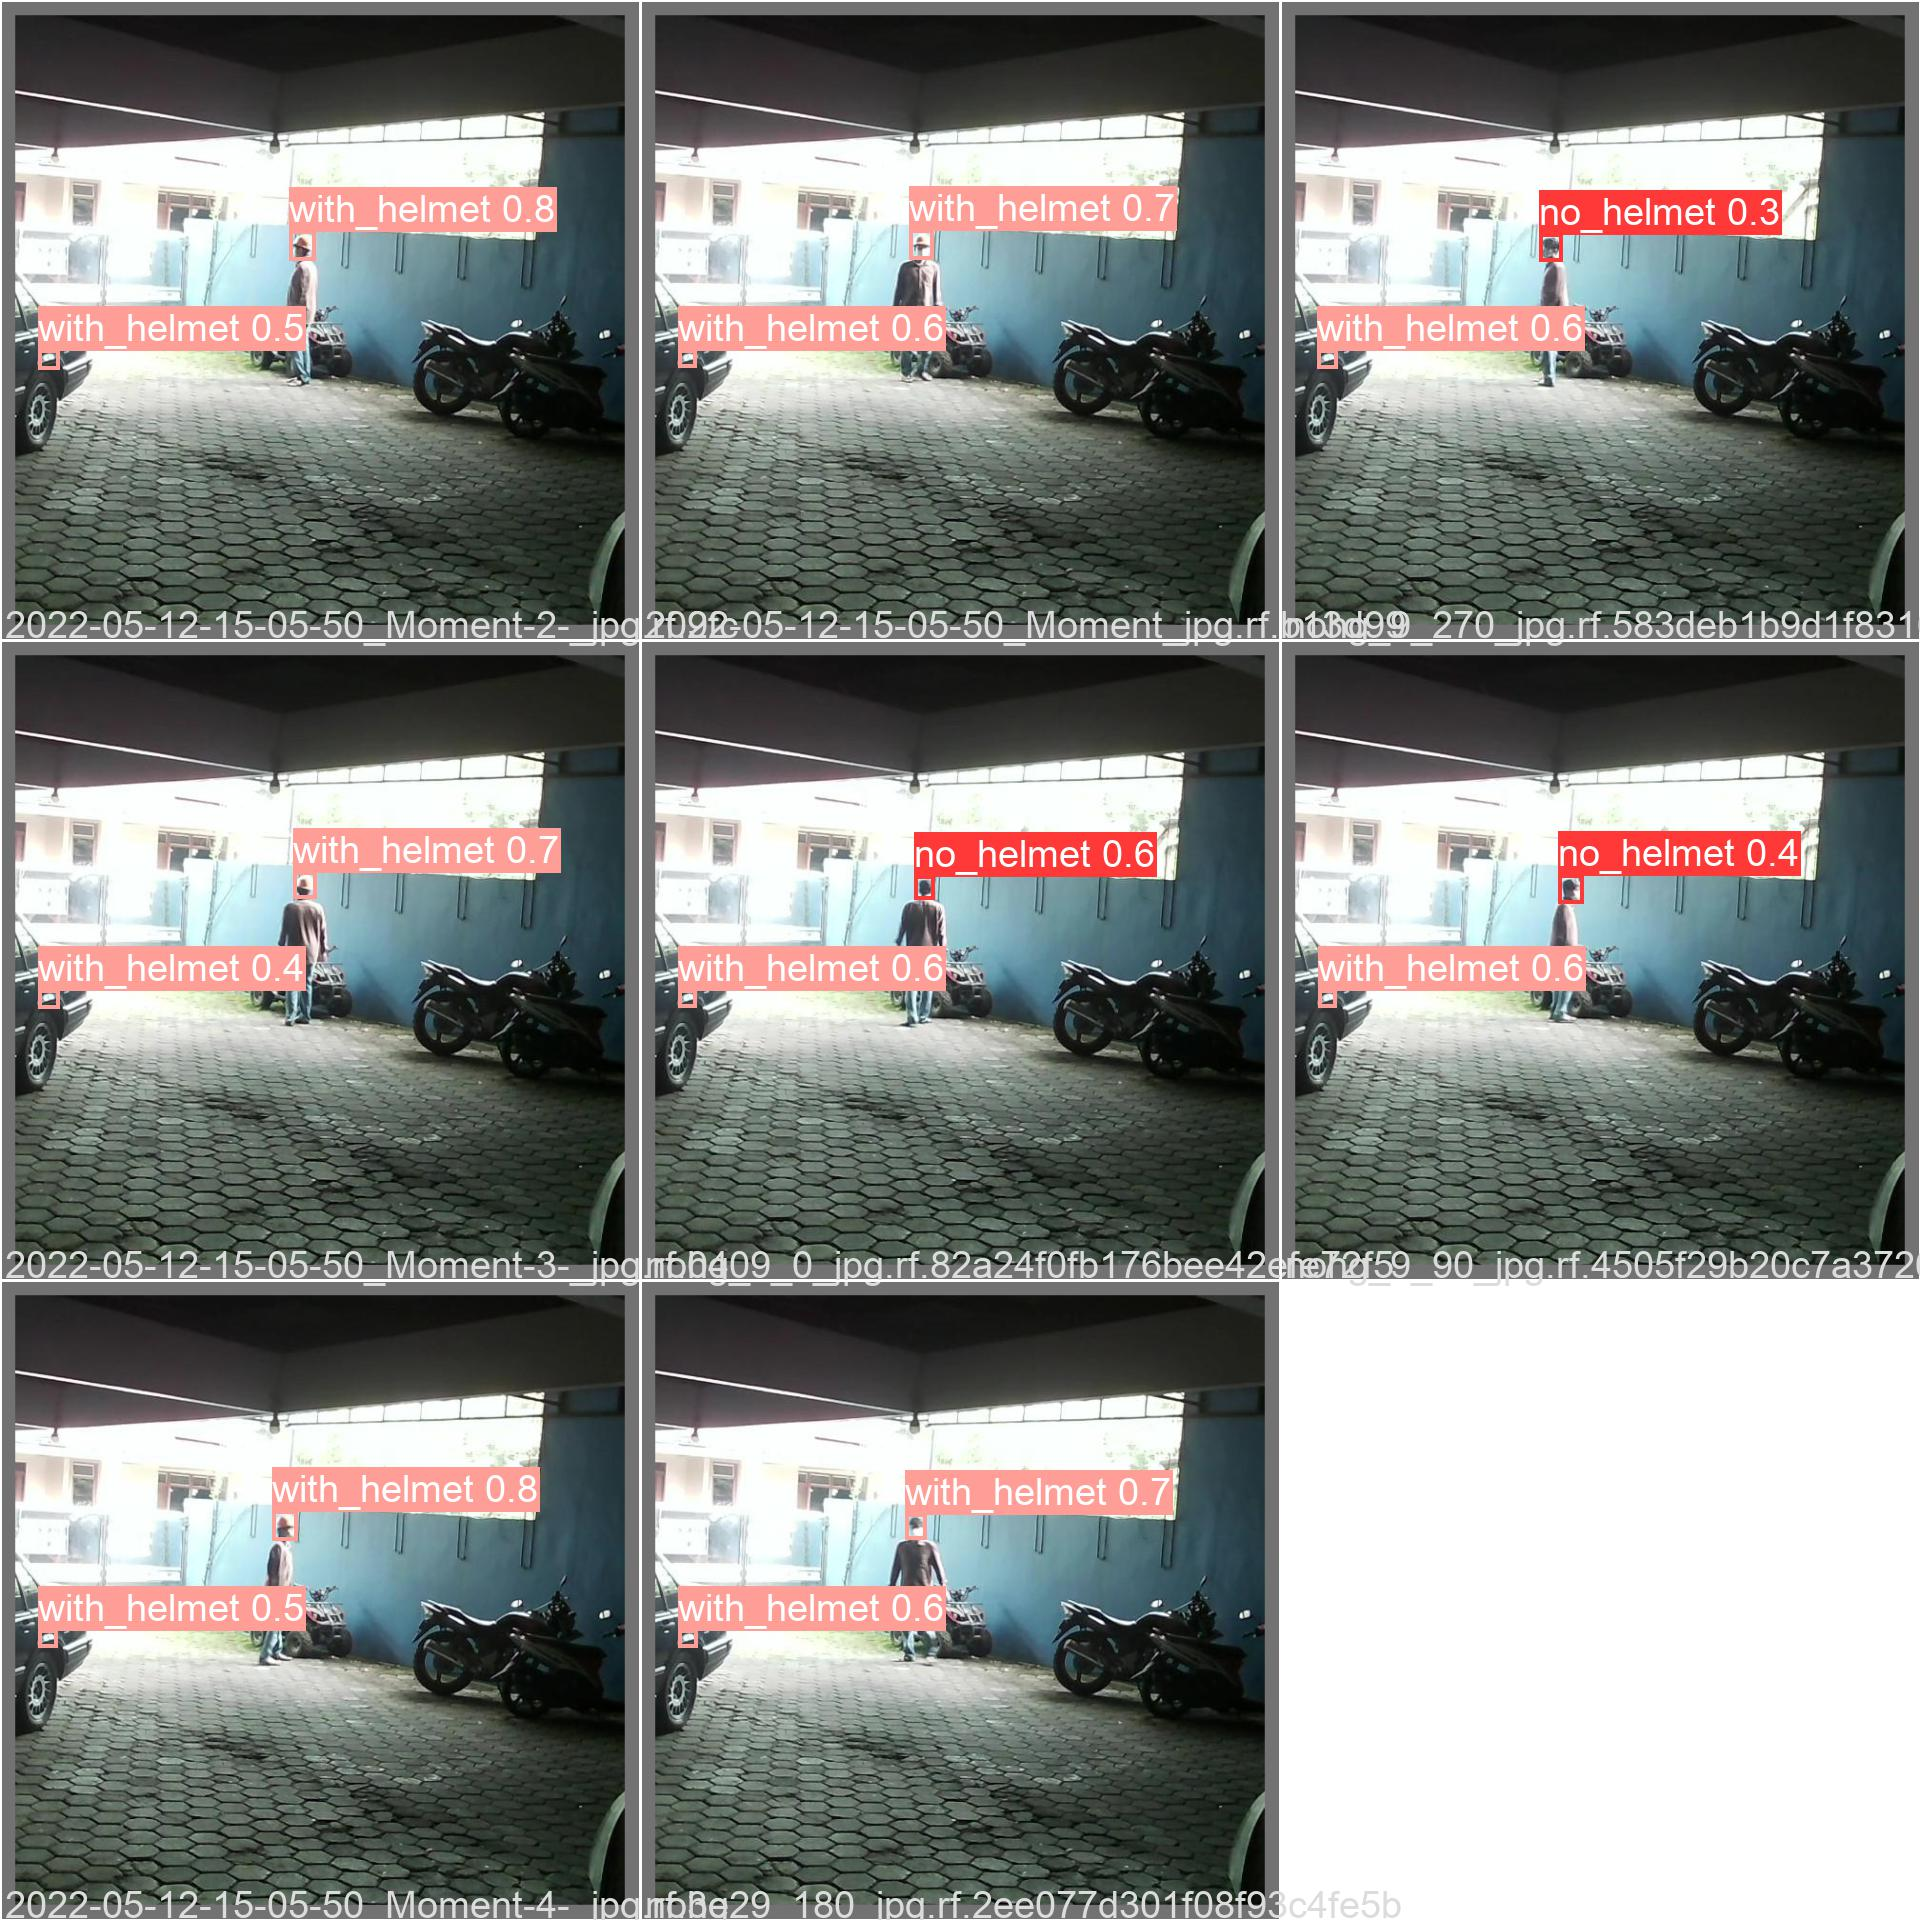
\includegraphics[width=0.31\textwidth]{gambar/BerdasarkanJarak_v2/val_hedec_pretrain_M/Jarak9/val_batch0_pred.jpg}
    \caption{Hasil Prediksi Untuk Bobot "hedec\_pretrain\_M" Pada Perbedaan Jarak}
    \label{fig:valjarak_sample_hedec_pretrain_M}  
  \end{figure}

   
  \item \textbf{hedec\_pretrain\_L}
  
  \par Pada pengujian menggunakan bobot "hedec\_pretrain\_L" pada perbedaan jarak, bobot ini memiliki hasil pengujian
  paling baik diantara bobot yang di\emph{train} menggunakan \emph{Pretrained Weights} dari YOLOv5 dimana untuk \emph{precision, recall,} dan \emph{mAP} berada di atas 0.9 untuk semua jarak
  dan kelas. Hasil validasi dapat dilihat pada Tabel~\ref{tb:hasiljarak_hedec_pretrain_L}.

  \par Seperti yang bisa dilihat dari Gambar~\ref{fig:grafvaljarak_hedec_pretrain_L}, hanya terjadi sedikit penurunan presisi
  pada jarak 1.3 meter untuk kelas "with\_helmet". Selain itu semua konstan di atas angka 0.98.


  \begin{longtable}{|l|l|l|l|l|} 
    \caption{Hasil Validasi Perbedaan Jarak Pada \textbf{"hedec\_pretrain\_L"}}
    \label{tb:hasiljarak_hedec_pretrain_L}\\
    \hline
    Jarak     & class        & precision & recall & mAP    \\ 
    \hline
    1.3 meter & all          & 0.984     & 1      & 0.995  \\
    2.6 meter & all          & 0.987     & 1      & 0.995  \\
    4 meter   & all          & 0.988     & 1      & 0.995  \\
    5.3 meter & all          & 0.988     & 1      & 0.995  \\
    6.7 meter & all          & 0.989     & 1      & 0.995  \\
    9 meter   & all          & 0.988     & 1      & 0.995  \\
    1.3 meter & no\_helmet   & 0.992     & 1      & 0.995  \\
    2.6 meter & no\_helmet   & 0.99      & 1      & 0.995  \\
    4 meter   & no\_helmet   & 0.989     & 1      & 0.995  \\
    5.3 meter & no\_helmet   & 0.99      & 1      & 0.995  \\
    6.7 meter & no\_helmet   & 0.99      & 1      & 0.995  \\
    9 meter   & no\_helmet   & 0.987     & 1      & 0.995  \\
    1.3 meter & with\_helmet & 0.975     & 1      & 0.995  \\
    2.6 meter & with\_helmet & 0.985     & 1      & 0.995  \\
    4 meter   & with\_helmet & 0.988     & 1      & 0.995  \\
    5.3 meter & with\_helmet & 0.985     & 1      & 0.995  \\
    6.7 meter & with\_helmet & 0.988     & 1      & 0.995  \\
    9 meter   & with\_helmet & 0.988     & 1      & 0.995  \\
    \hline
  \end{longtable}

  \begin{figure} [h!]
    \centering
    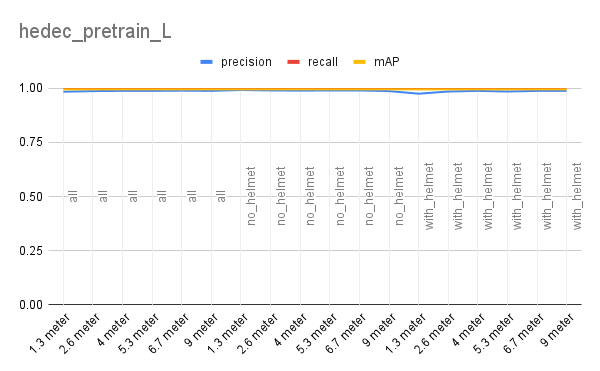
\includegraphics[width=1\textwidth]{gambar/BerdasarkanJarak/hedec_pretrain_L.png}
    \caption{Grafik \emph{Precision, Recall, mAP} untuk \textbf{"hedec\_pretrain\_L"} Pada Jarak 1.3 meter Hingga 9 meter}
    \label{fig:grafvaljarak_hedec_pretrain_L}  
  \end{figure}

  \begin{figure} [h!]
    \centering
    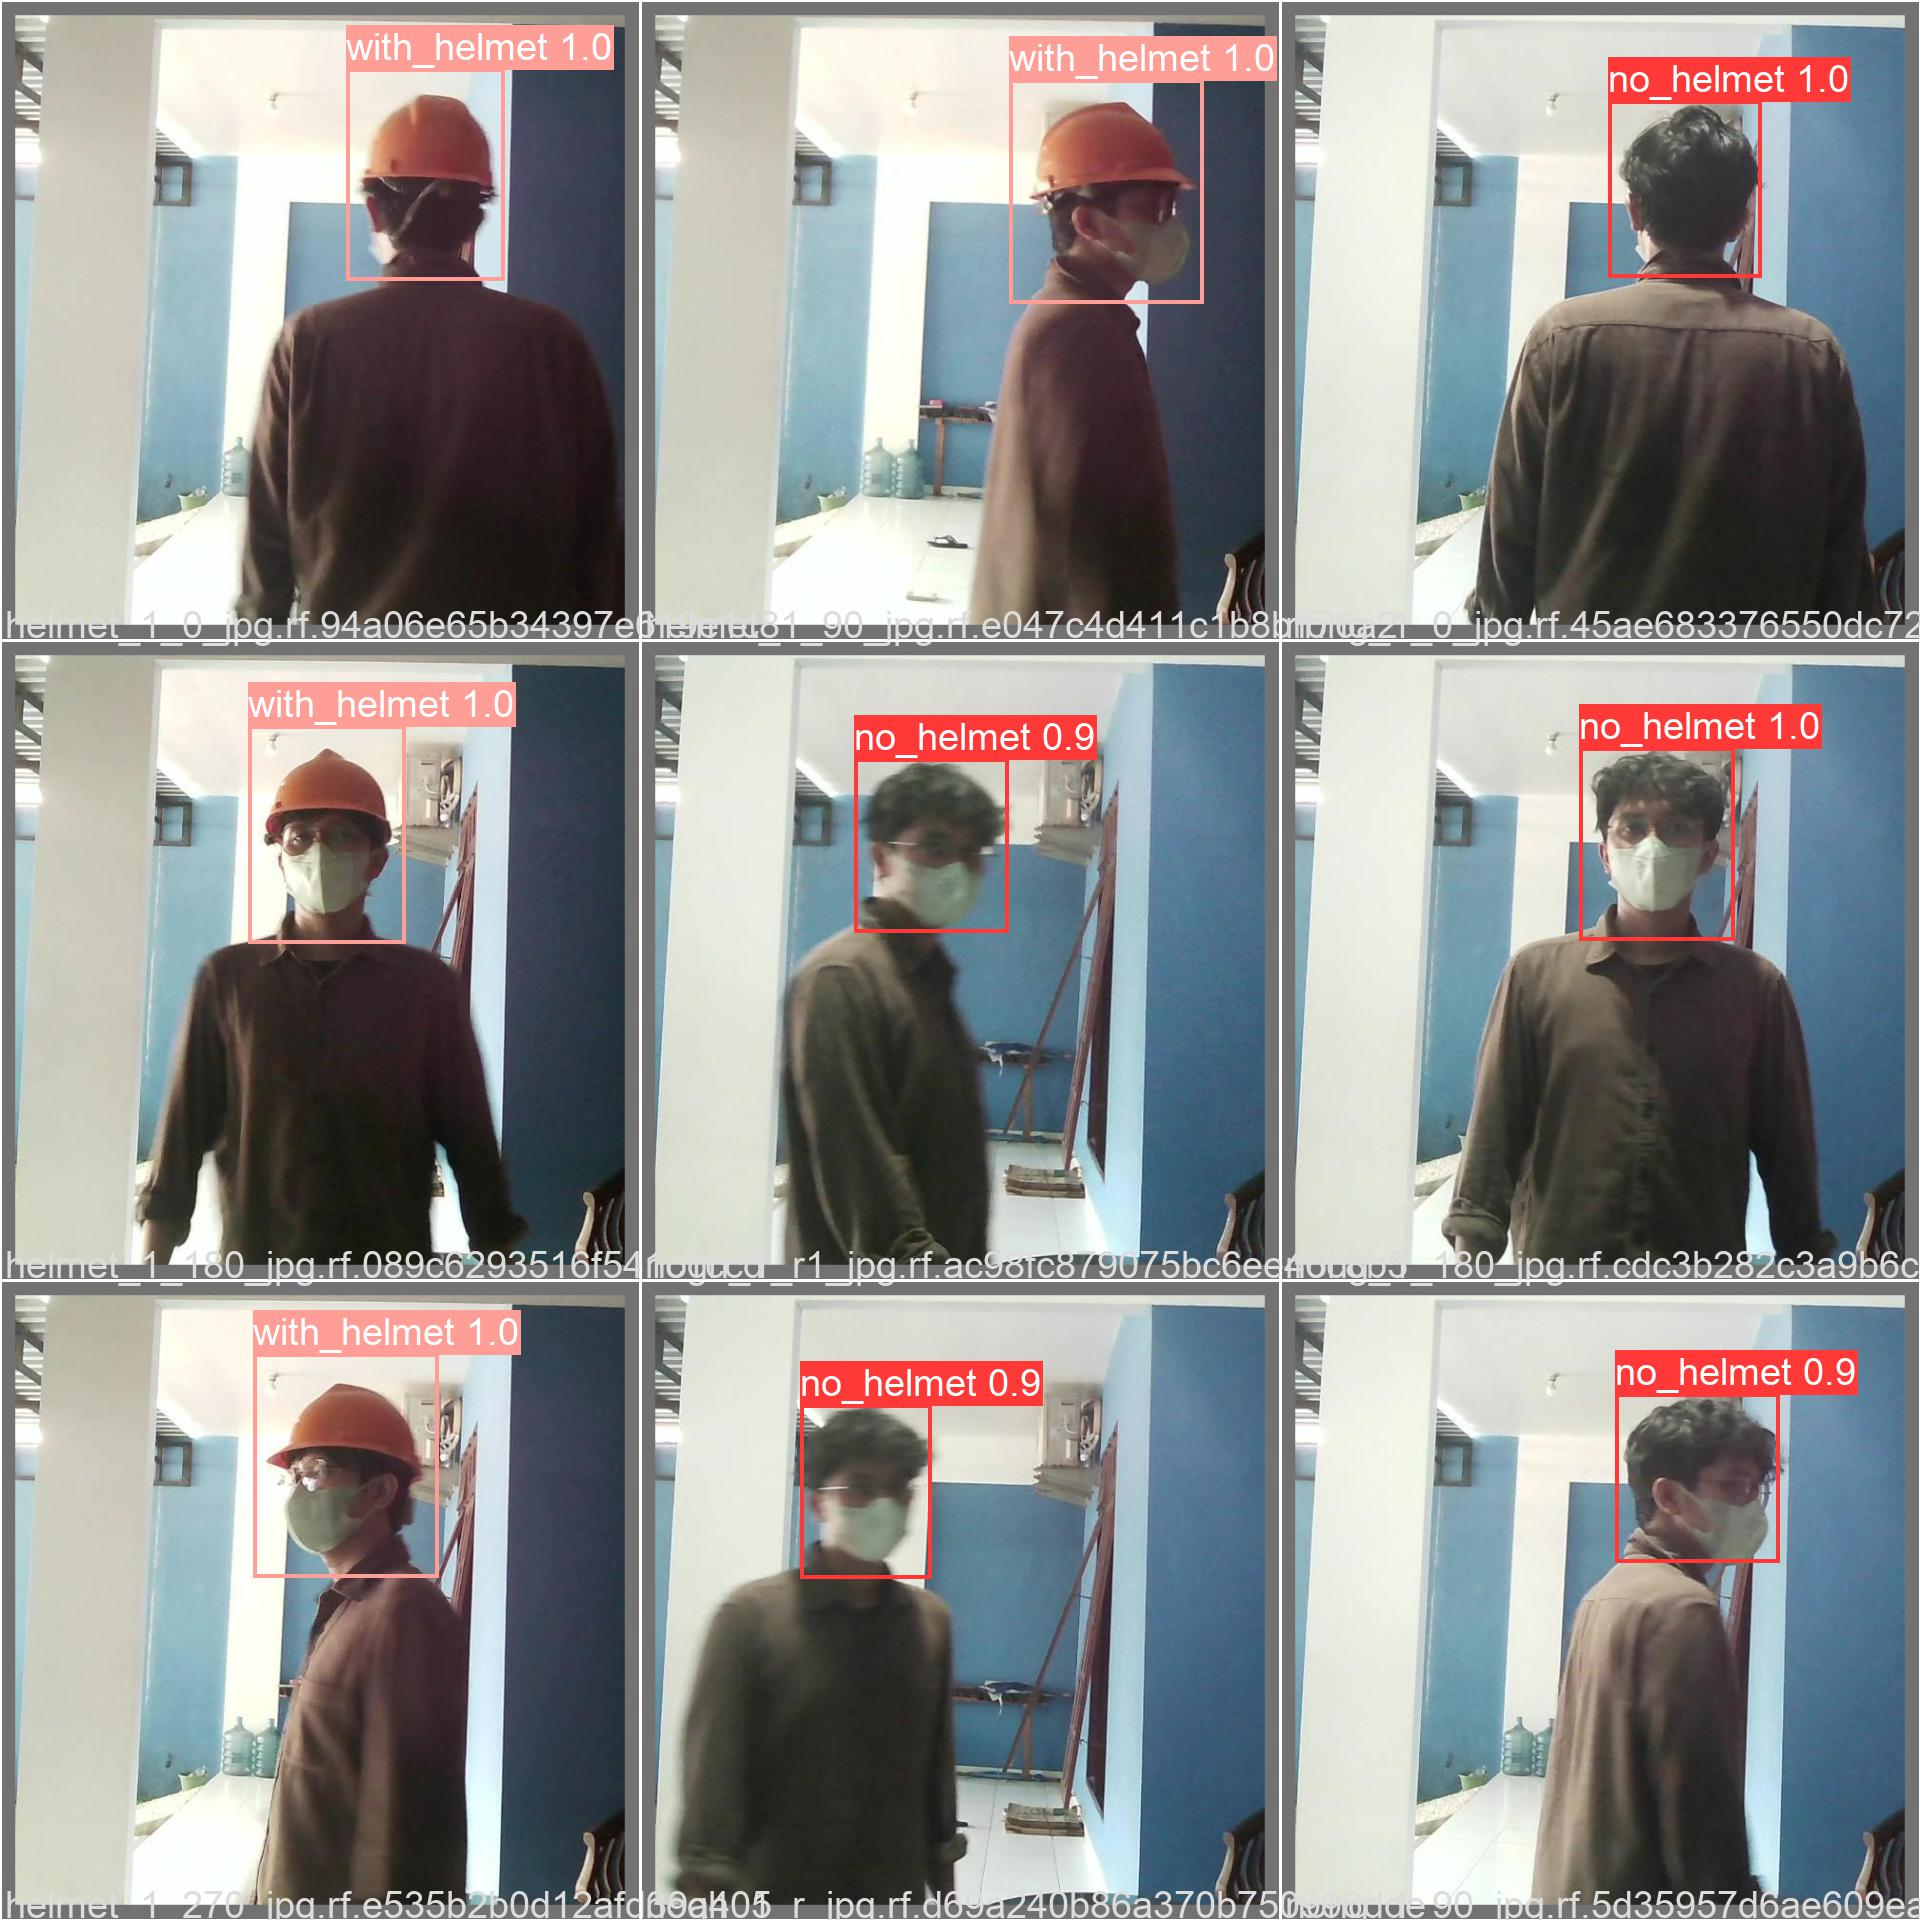
\includegraphics[width=0.31\textwidth]{gambar/BerdasarkanJarak_v2/val_hedec_pretrain_L/Jarak1_3/val_batch0_pred.jpg}
    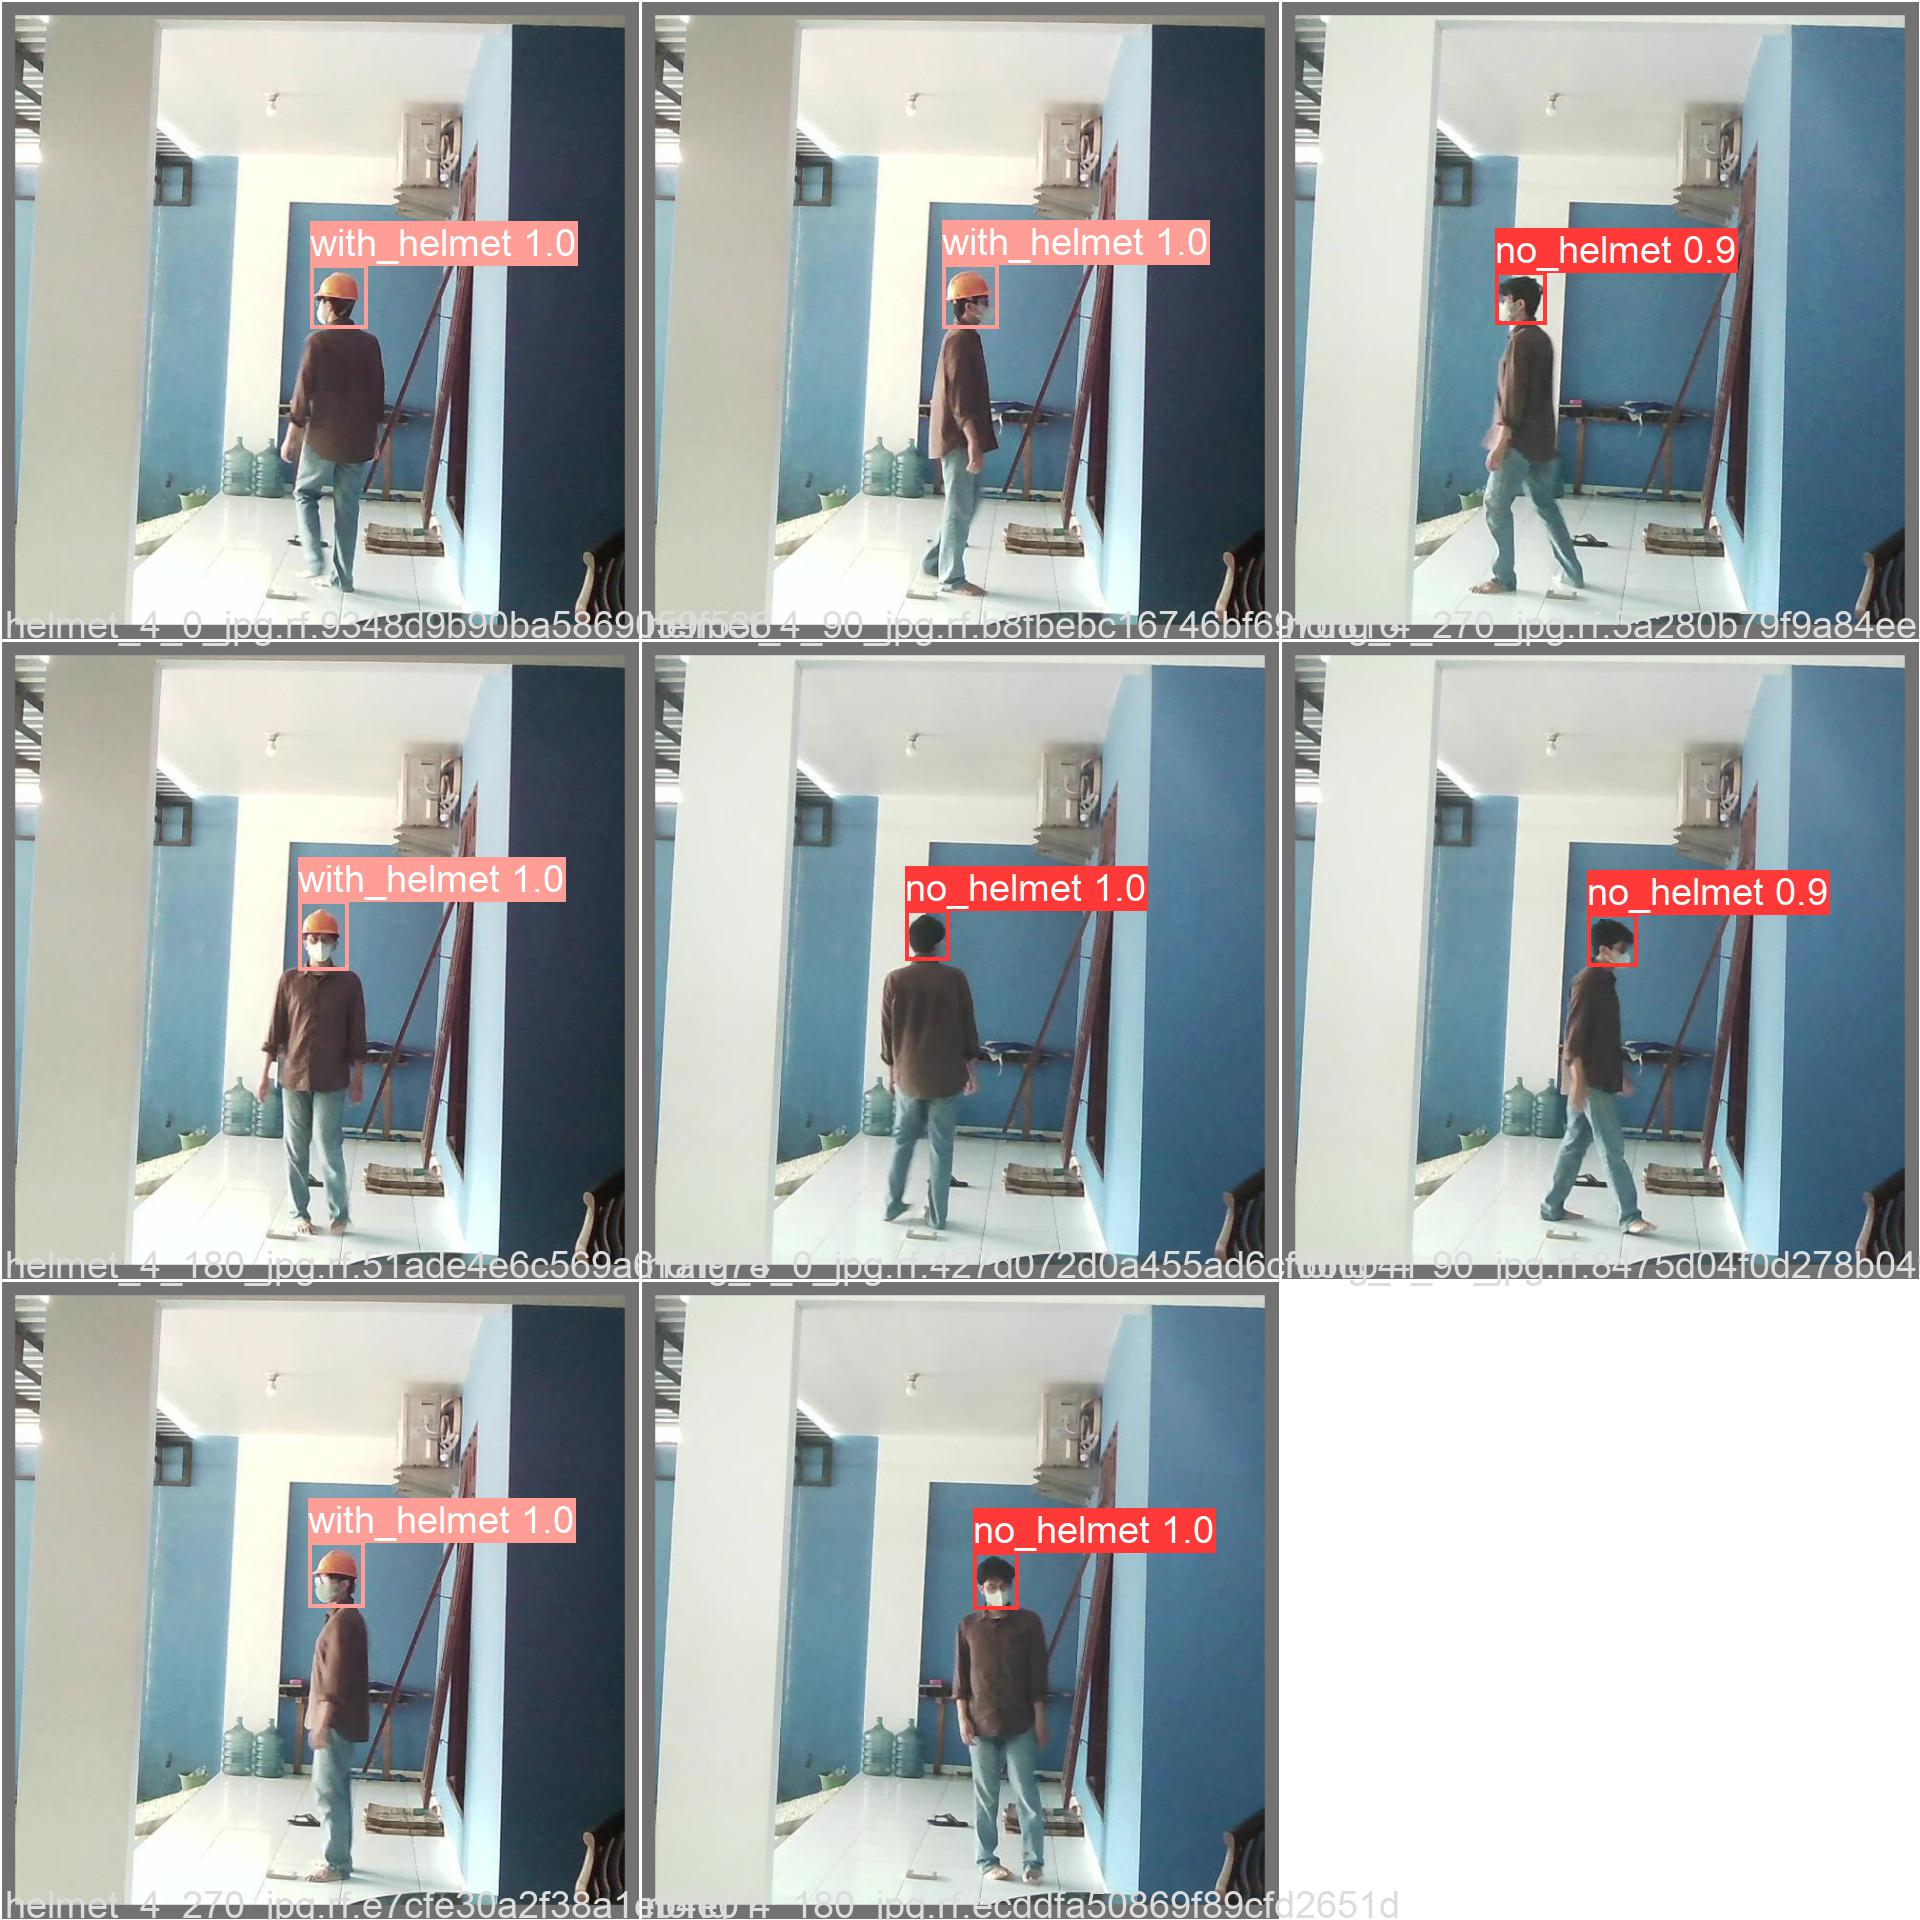
\includegraphics[width=0.31\textwidth]{gambar/BerdasarkanJarak_v2/val_hedec_pretrain_L/Jarak5_3/val_batch0_pred.jpg}
    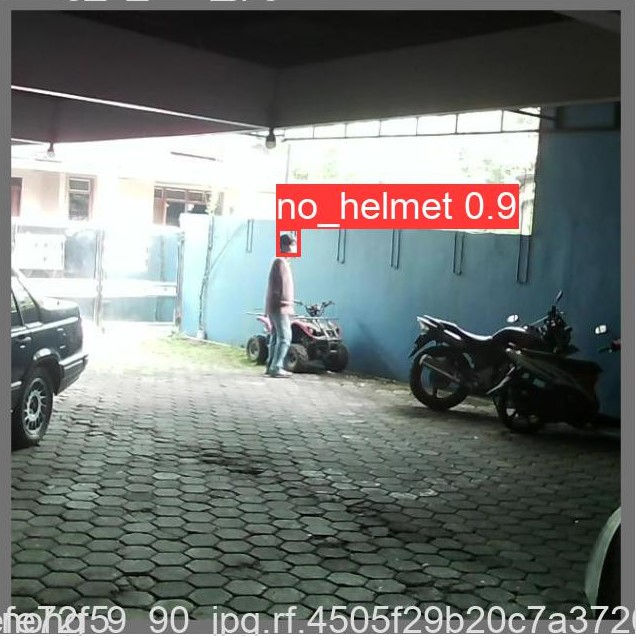
\includegraphics[width=0.31\textwidth]{gambar/BerdasarkanJarak_v2/val_hedec_pretrain_L/Jarak9/val_batch0_pred.jpg}
    \caption{Hasil Prediksi Untuk Bobot "hedec\_pretrain\_L" Pada Perbedaan Jarak}
    \label{fig:valjarak_sample_hedec_pretrain_L}  
  \end{figure}

\end{enumerate}


\newpage
\subsection{Pengujian Jarak dengan \emph{Pure Weight}}
\label{subsec:ujijarak_pureweight}

\par Bagian ini memaparkan pengujian menggunakan bobot hasil \emph{training} tanpa menggunakan \emph{Pretrained Weights}
dari repo YOLOv5 yang selanjutnya disebut sebagai "hedec\_pure". 

\begin{enumerate}
  \item \textbf{hedec\_pure\_N}
  \par Pada bagian dipaparkan hasil pengujian dari bobot "hedec\_pure\_N" yang merupakan bobot hasil \emph{training}
  yang tidak menggunakan \emph{Pretrained Weights} dari repository YOLOv5 tetapi konfigurasinya menyerupai konfigurasi
  varian \emph{Pretrained Weights} varian YOLOv5n. Seperti yang ditunjukkan pada Gambar~\ref{fig:grafvaljarak_hedec_pure_N}
  , untuk semua kelas memiliki nilai \emph{precision} di atas 0.8 untuk semua jarak. Tetapi untuk \emph{recall} pada jarak 1.3 meter
  untuk kelas "no\_helmet" memiliki nilai 0.6 dimana terdapat kegagalan memprediksi kelas "no\_helmet" dan prediksi lokasi yang
  kurang akurat. Tabel Hasil Validasi bobot "hedec\_pure\_N" bisa dilihat pada Tabel~\ref{tb:hasiljarak_hedec_pure_N}.

  \begin{figure} [h!]
    \centering
    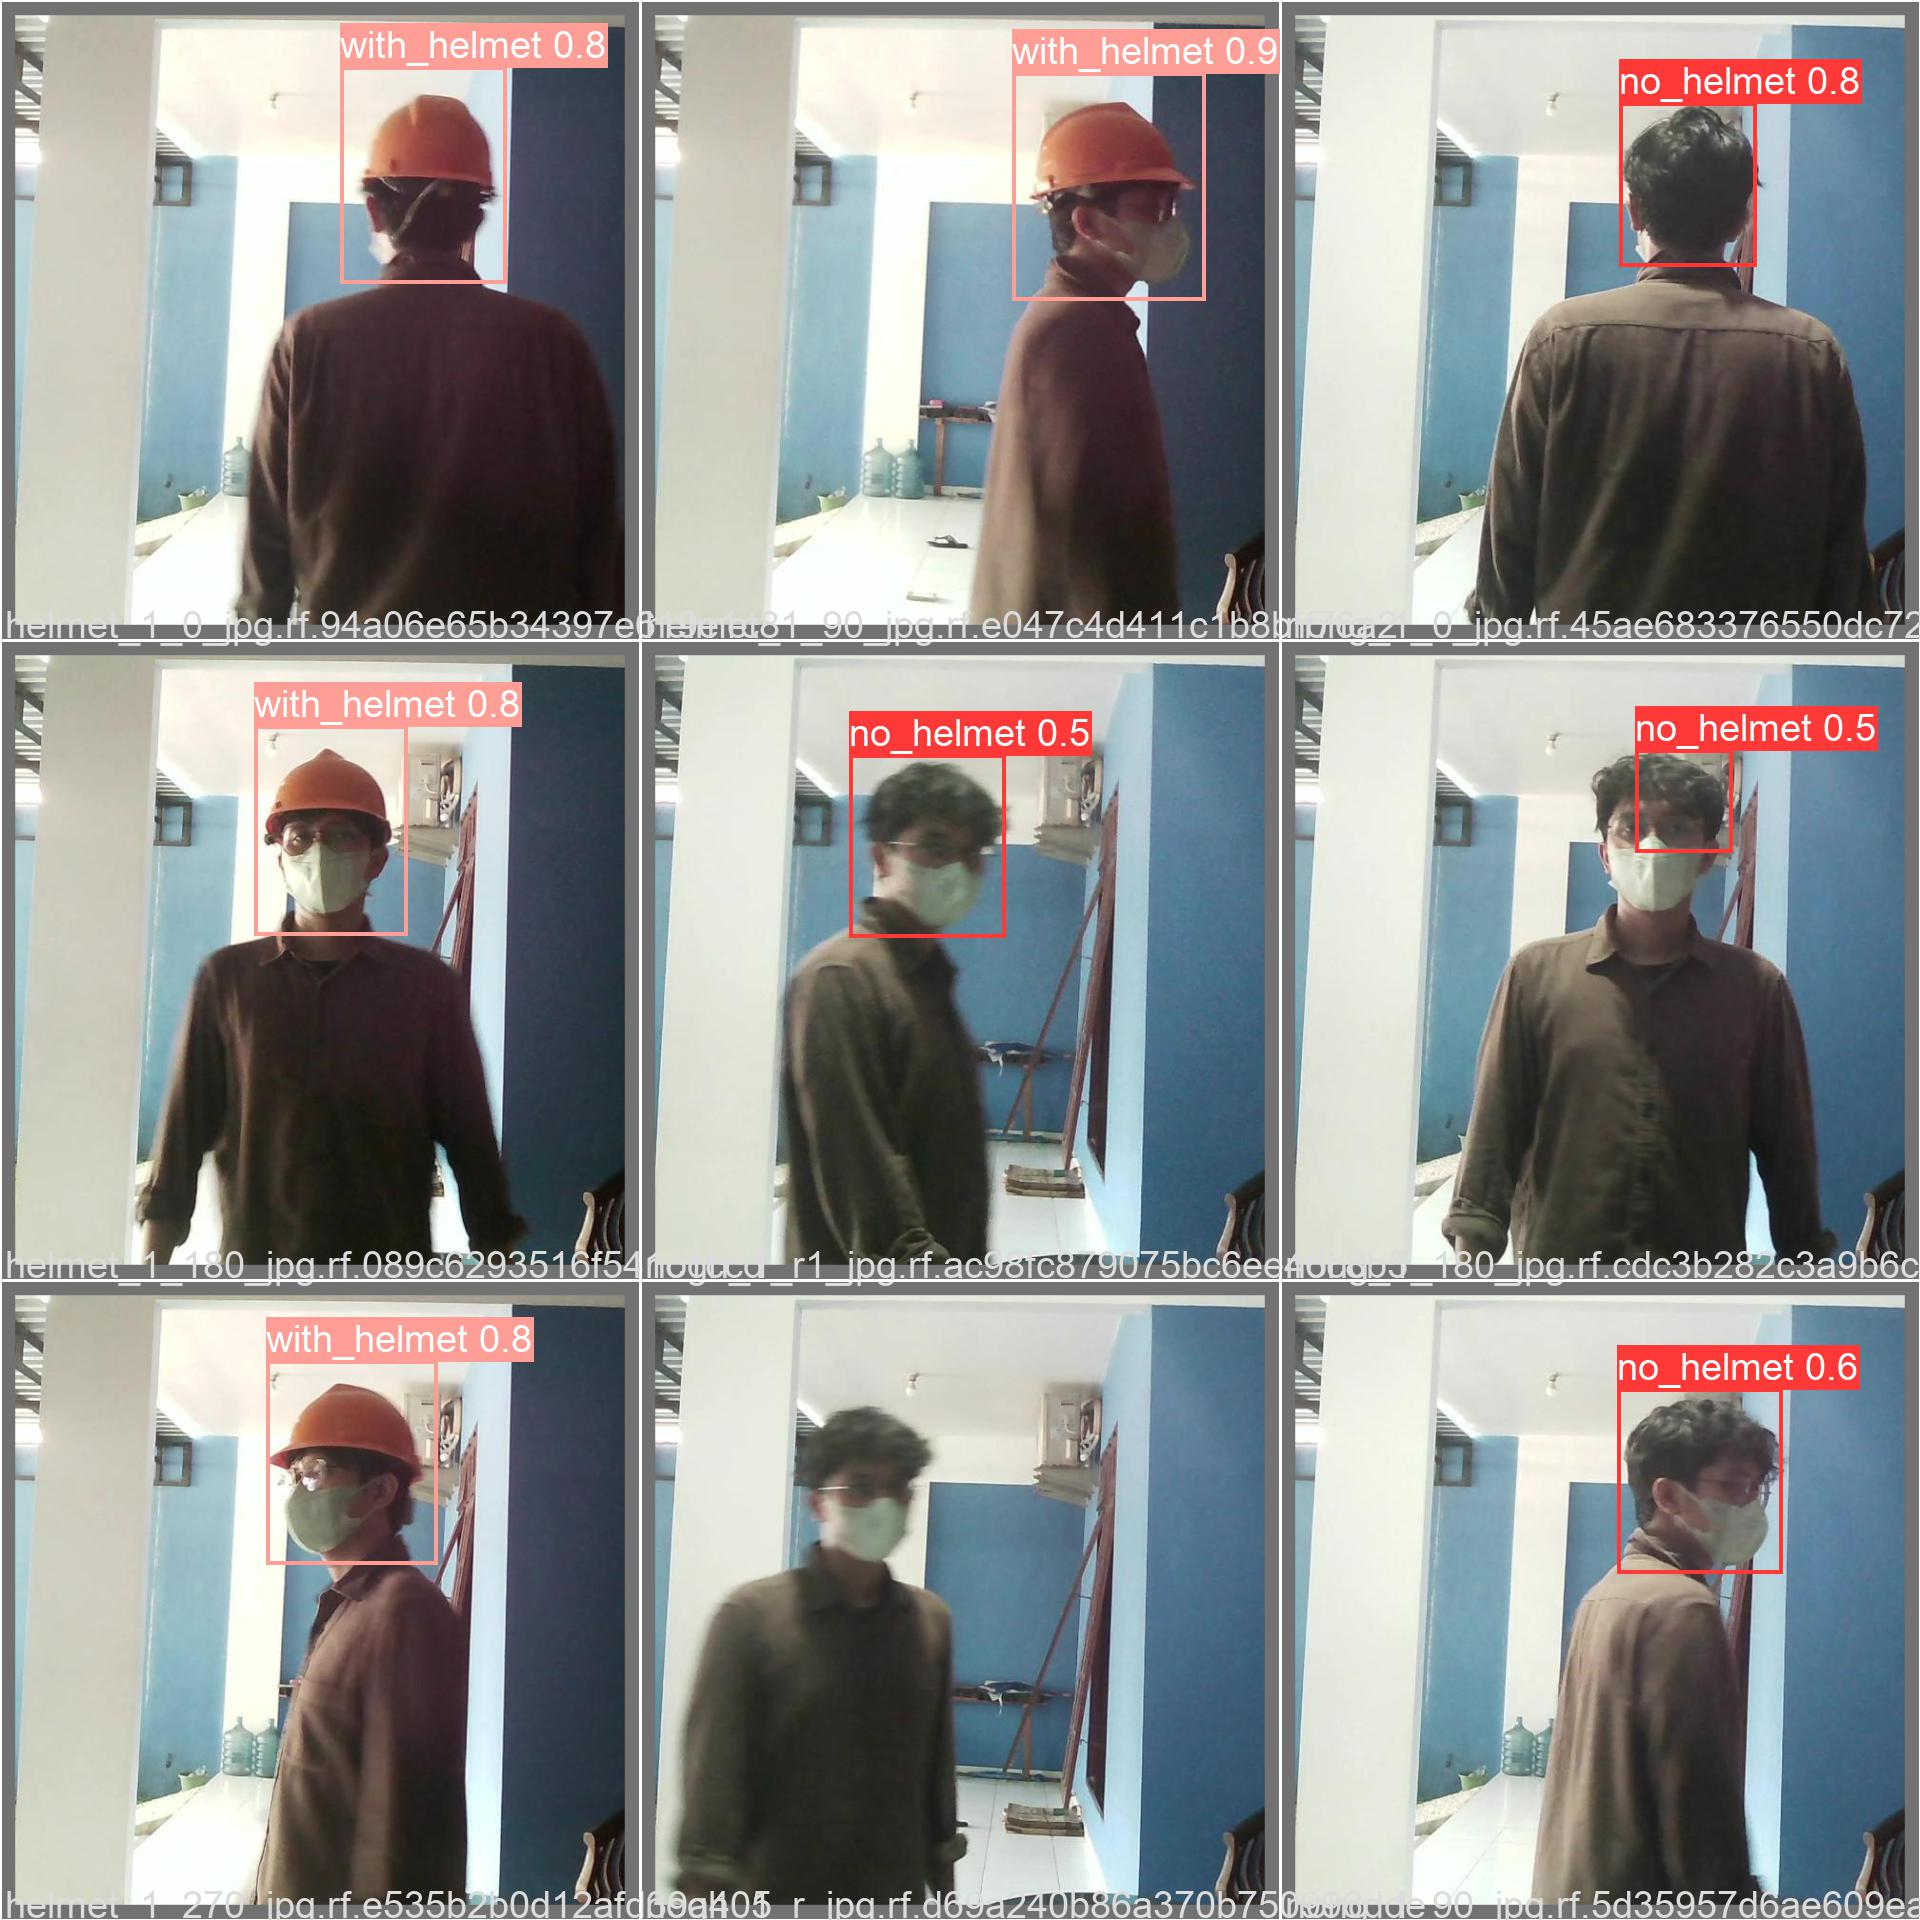
\includegraphics[width=0.31\textwidth]{gambar/BerdasarkanJarak_v2/val_hedec_pure_N/Jarak1_3/val_batch0_pred.jpg}
    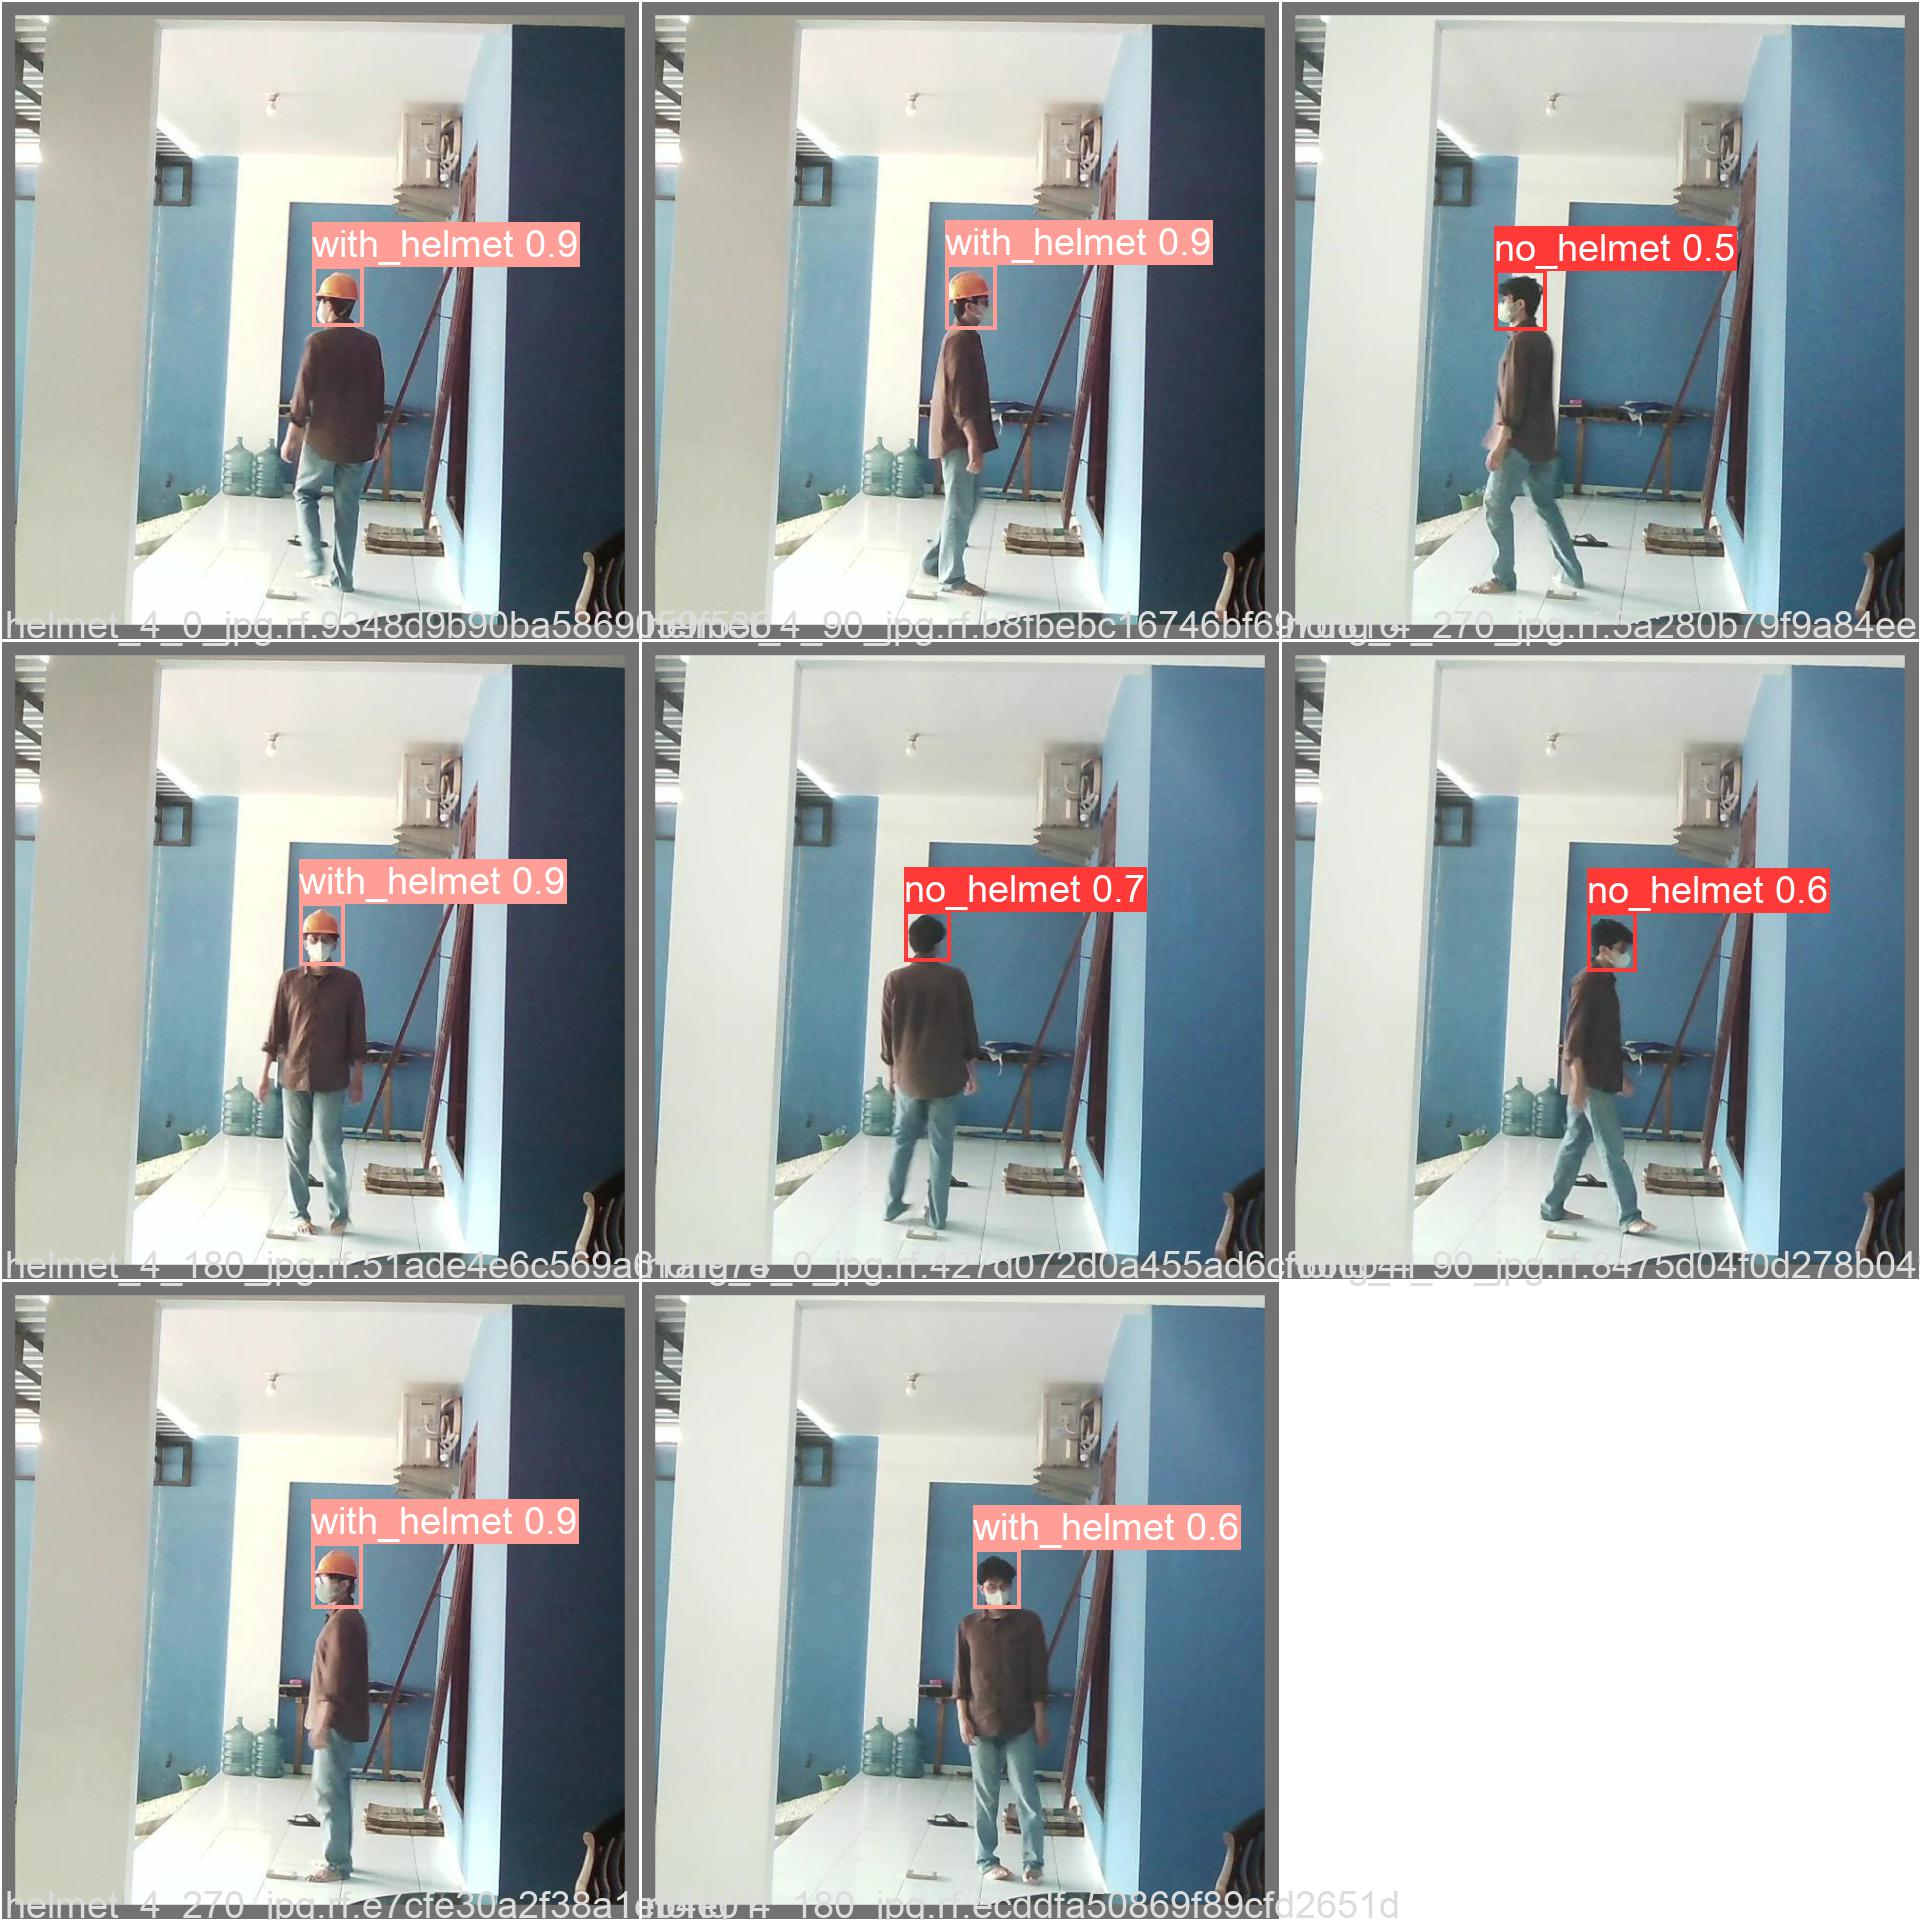
\includegraphics[width=0.31\textwidth]{gambar/BerdasarkanJarak_v2/val_hedec_pure_N/Jarak5_3/val_batch0_pred.jpg}
    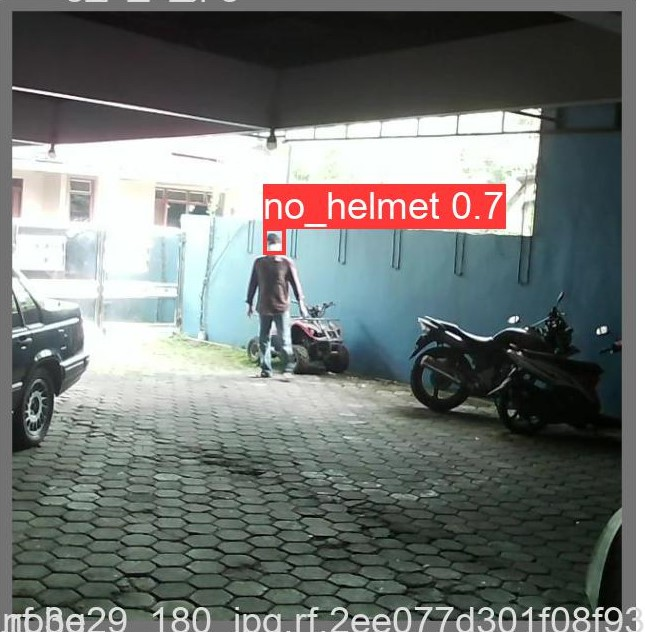
\includegraphics[width=0.31\textwidth]{gambar/BerdasarkanJarak_v2/val_hedec_pure_N/Jarak9/val_batch0_pred.jpg}
    \caption{Hasil Prediksi Untuk Bobot "hedec\_pure\_N" Pada Perbedaan Jarak}
    \label{fig:valjarak_sample_hedec_pure_N}  
  \end{figure}

  \begin{longtable}{|l|l|l|l|l|} 
    \caption{Hasil Validasi Perbedaan Jarak Pada \textbf{"hedec\_pure\_N"}}
    \label{tb:hasiljarak_hedec_pure_N}\\
    \hline
      Jarak     & class        & precision & recall & mAP    \\ 
      \hline
      1.3 meter & all          & 0.889     & 0.8    & 0.903  \\
      2.6 meter & all          & 0.971     & 1      & 0.995  \\
      4 meter   & all          & 0.904     & 0.986  & 0.995  \\
      5.3 meter & all          & 0.847     & 0.989  & 0.995  \\
      6.7 meter & all          & 0.949     & 1      & 0.995  \\
      9 meter   & all          & 0.92      & 1      & 0.995  \\
      1.3 meter & no\_helmet   & 0.876     & 0.6    & 0.812  \\
      2.6 meter & no\_helmet   & 0.991     & 1      & 0.995  \\
      4 meter   & no\_helmet   & 1         & 0.971  & 0.995  \\
      5.3 meter & no\_helmet   & 1         & 0.977  & 0.995  \\
      6.7 meter & no\_helmet   & 0.997     & 1      & 0.995  \\
      9 meter   & no\_helmet   & 0.979     & 1      & 0.995  \\
      1.3 meter & with\_helmet & 0.902     & 1      & 0.995  \\
      2.6 meter & with\_helmet & 0.952     & 1      & 0.995  \\
      4 meter   & with\_helmet & 0.808     & 1      & 0.995  \\
      5.3 meter & with\_helmet & 0.694     & 1      & 0.995  \\
      6.7 meter & with\_helmet & 0.901     & 1      & 0.995  \\
      9 meter   & with\_helmet & 0.861     & 1      & 0.995  \\
      \hline
  \end{longtable}

  \begin{figure} [h!]
    \centering
    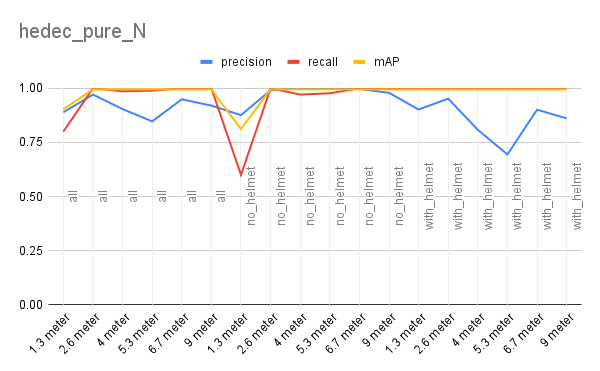
\includegraphics[width=1\textwidth]{gambar/BerdasarkanJarak/hedec_pure_N.png}
    \caption{Grafik \emph{Precision, Recall, mAP} untuk \textbf{"hedec\_pure\_N"} Pada Jarak 1.3 meter Hingga 9 meter}
    \label{fig:grafvaljarak_hedec_pure_N}  
  \end{figure}

  

  \FloatBarrier


  \item \textbf{hedec\_pure\_S}
  
  \par Pada pengujian pada jarak berbeda dari 1.3 meter hingga 9 meter untuk bobot "hedec\_pure\_S" yang merupakan bobot hasil \emph{training}
  yang tidak menggunakan \emph{Pretrained Weights} dari repository YOLOv5 tetapi konfigurasinya menyerupai konfigurasi
  varian \emph{Pretrained Weights} varian YOLOv5s ini ditemukan beberapa hal. Seperti yang bisa dilihat pada Gambar~\ref{fig:grafvaljarak_hedec_pure_S},
  pada jarak 1.3 meter memiliki nilai yang rendah untuk \emph{precision, recall} dan juga nilai mAP nya dimana untuk kelas "no\_helmet" didapati kesalahan prediksi. Lalu mulai dari
  jarak 2.6 meter hingga 6.7 meter mengalami kenaikan. Tetapi pada jarak 9 meter, \emph{precision} untuk kelas "with\_helmet"
  mengalami penurunan karena ada kelas "no\_helmet" yang terdeteksi sebagai "with\_helmet". Tabel untuk hasil validasi dari "hedec\_pure\_N" bisa dilihat
  pada Tabel~\ref{tb:hasiljarak_hedec_pure_S}.
  
  \begin{longtable}{|l|l|l|l|l|} 
    \caption{Hasil Validasi Perbedaan Jarak Pada \textbf{"hedec\_pure\_S"}}
    \label{tb:hasiljarak_hedec_pure_S}\\
    \hline
    Jarak     & class        & precision & recall & mAP    \\ 
    \hline
    1.3 meter & all          & 0.846     & 0.8    & 0.891  \\
    2.6 meter & all          & 0.978     & 1      & 0.995  \\
    4 meter   & all          & 0.959     & 1      & 0.995  \\
    5.3 meter & all          & 0.891     & 1      & 0.995  \\
    6.7 meter & all          & 0.948     & 1      & 0.995  \\
    9 meter   & all          & 0.745     & 1      & 0.97   \\
    1.3 meter & no\_helmet   & 0.728     & 0.6    & 0.787  \\
    2.6 meter & no\_helmet   & 0.991     & 1      & 0.995  \\
    4 meter   & no\_helmet   & 0.987     & 1      & 0.995  \\
    5.3 meter & no\_helmet   & 0.985     & 1      & 0.995  \\
    6.7 meter & no\_helmet   & 0.994     & 1      & 0.995  \\
    9 meter   & no\_helmet   & 0.981     & 1      & 0.995  \\
    1.3 meter & with\_helmet & 0.964     & 1      & 0.995  \\
    2.6 meter & with\_helmet & 0.965     & 1      & 0.995  \\
    4 meter   & with\_helmet & 0.93      & 1      & 0.995  \\
    5.3 meter & with\_helmet & 0.797     & 1      & 0.995  \\
    6.7 meter & with\_helmet & 0.901     & 1      & 0.995  \\
    9 meter   & with\_helmet & 0.508     & 1      & 0.945  \\
    \hline
  \end{longtable}

  \begin{figure} [h!]
    \centering
    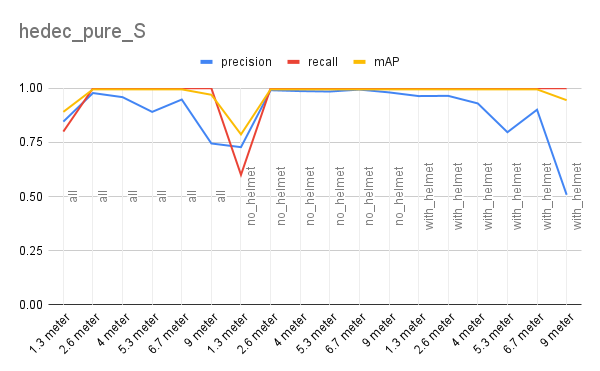
\includegraphics[width=1\textwidth]{gambar/BerdasarkanJarak/hedec_pure_S.png}
    \caption{Grafik \emph{Precision, Recall, mAP} untuk \textbf{"hedec\_pure\_S"} Pada Jarak 1.3 meter Hingga 9 meter}
    \label{fig:grafvaljarak_hedec_pure_S}  
  \end{figure}

  \begin{figure} [h!]
    \centering
    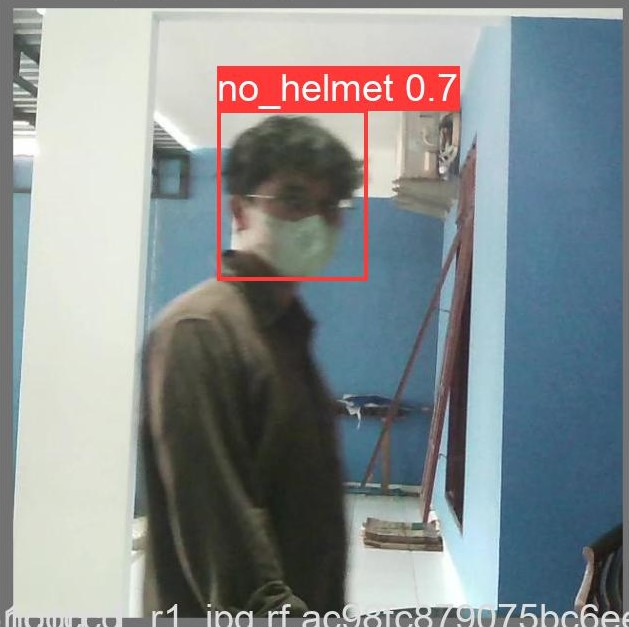
\includegraphics[width=0.31\textwidth]{gambar/BerdasarkanJarak_v2/val_hedec_pure_S/Jarak1_3/val_batch0_pred.jpg}
    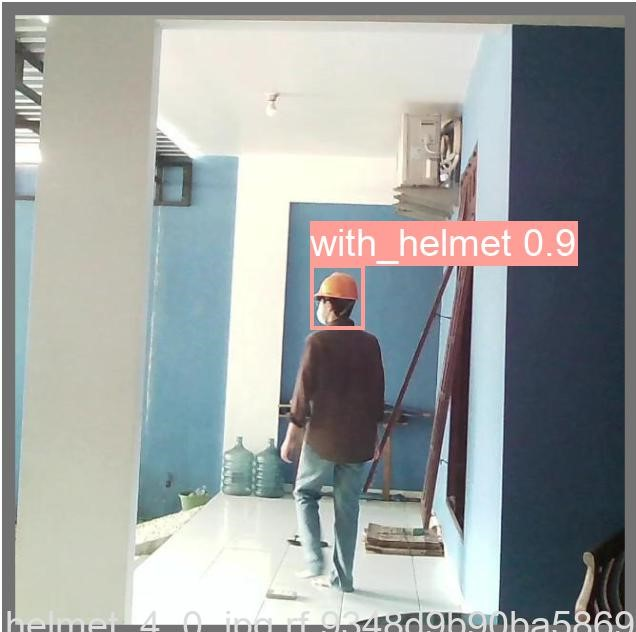
\includegraphics[width=0.31\textwidth]{gambar/BerdasarkanJarak_v2/val_hedec_pure_S/Jarak5_3/val_batch0_pred.jpg}
    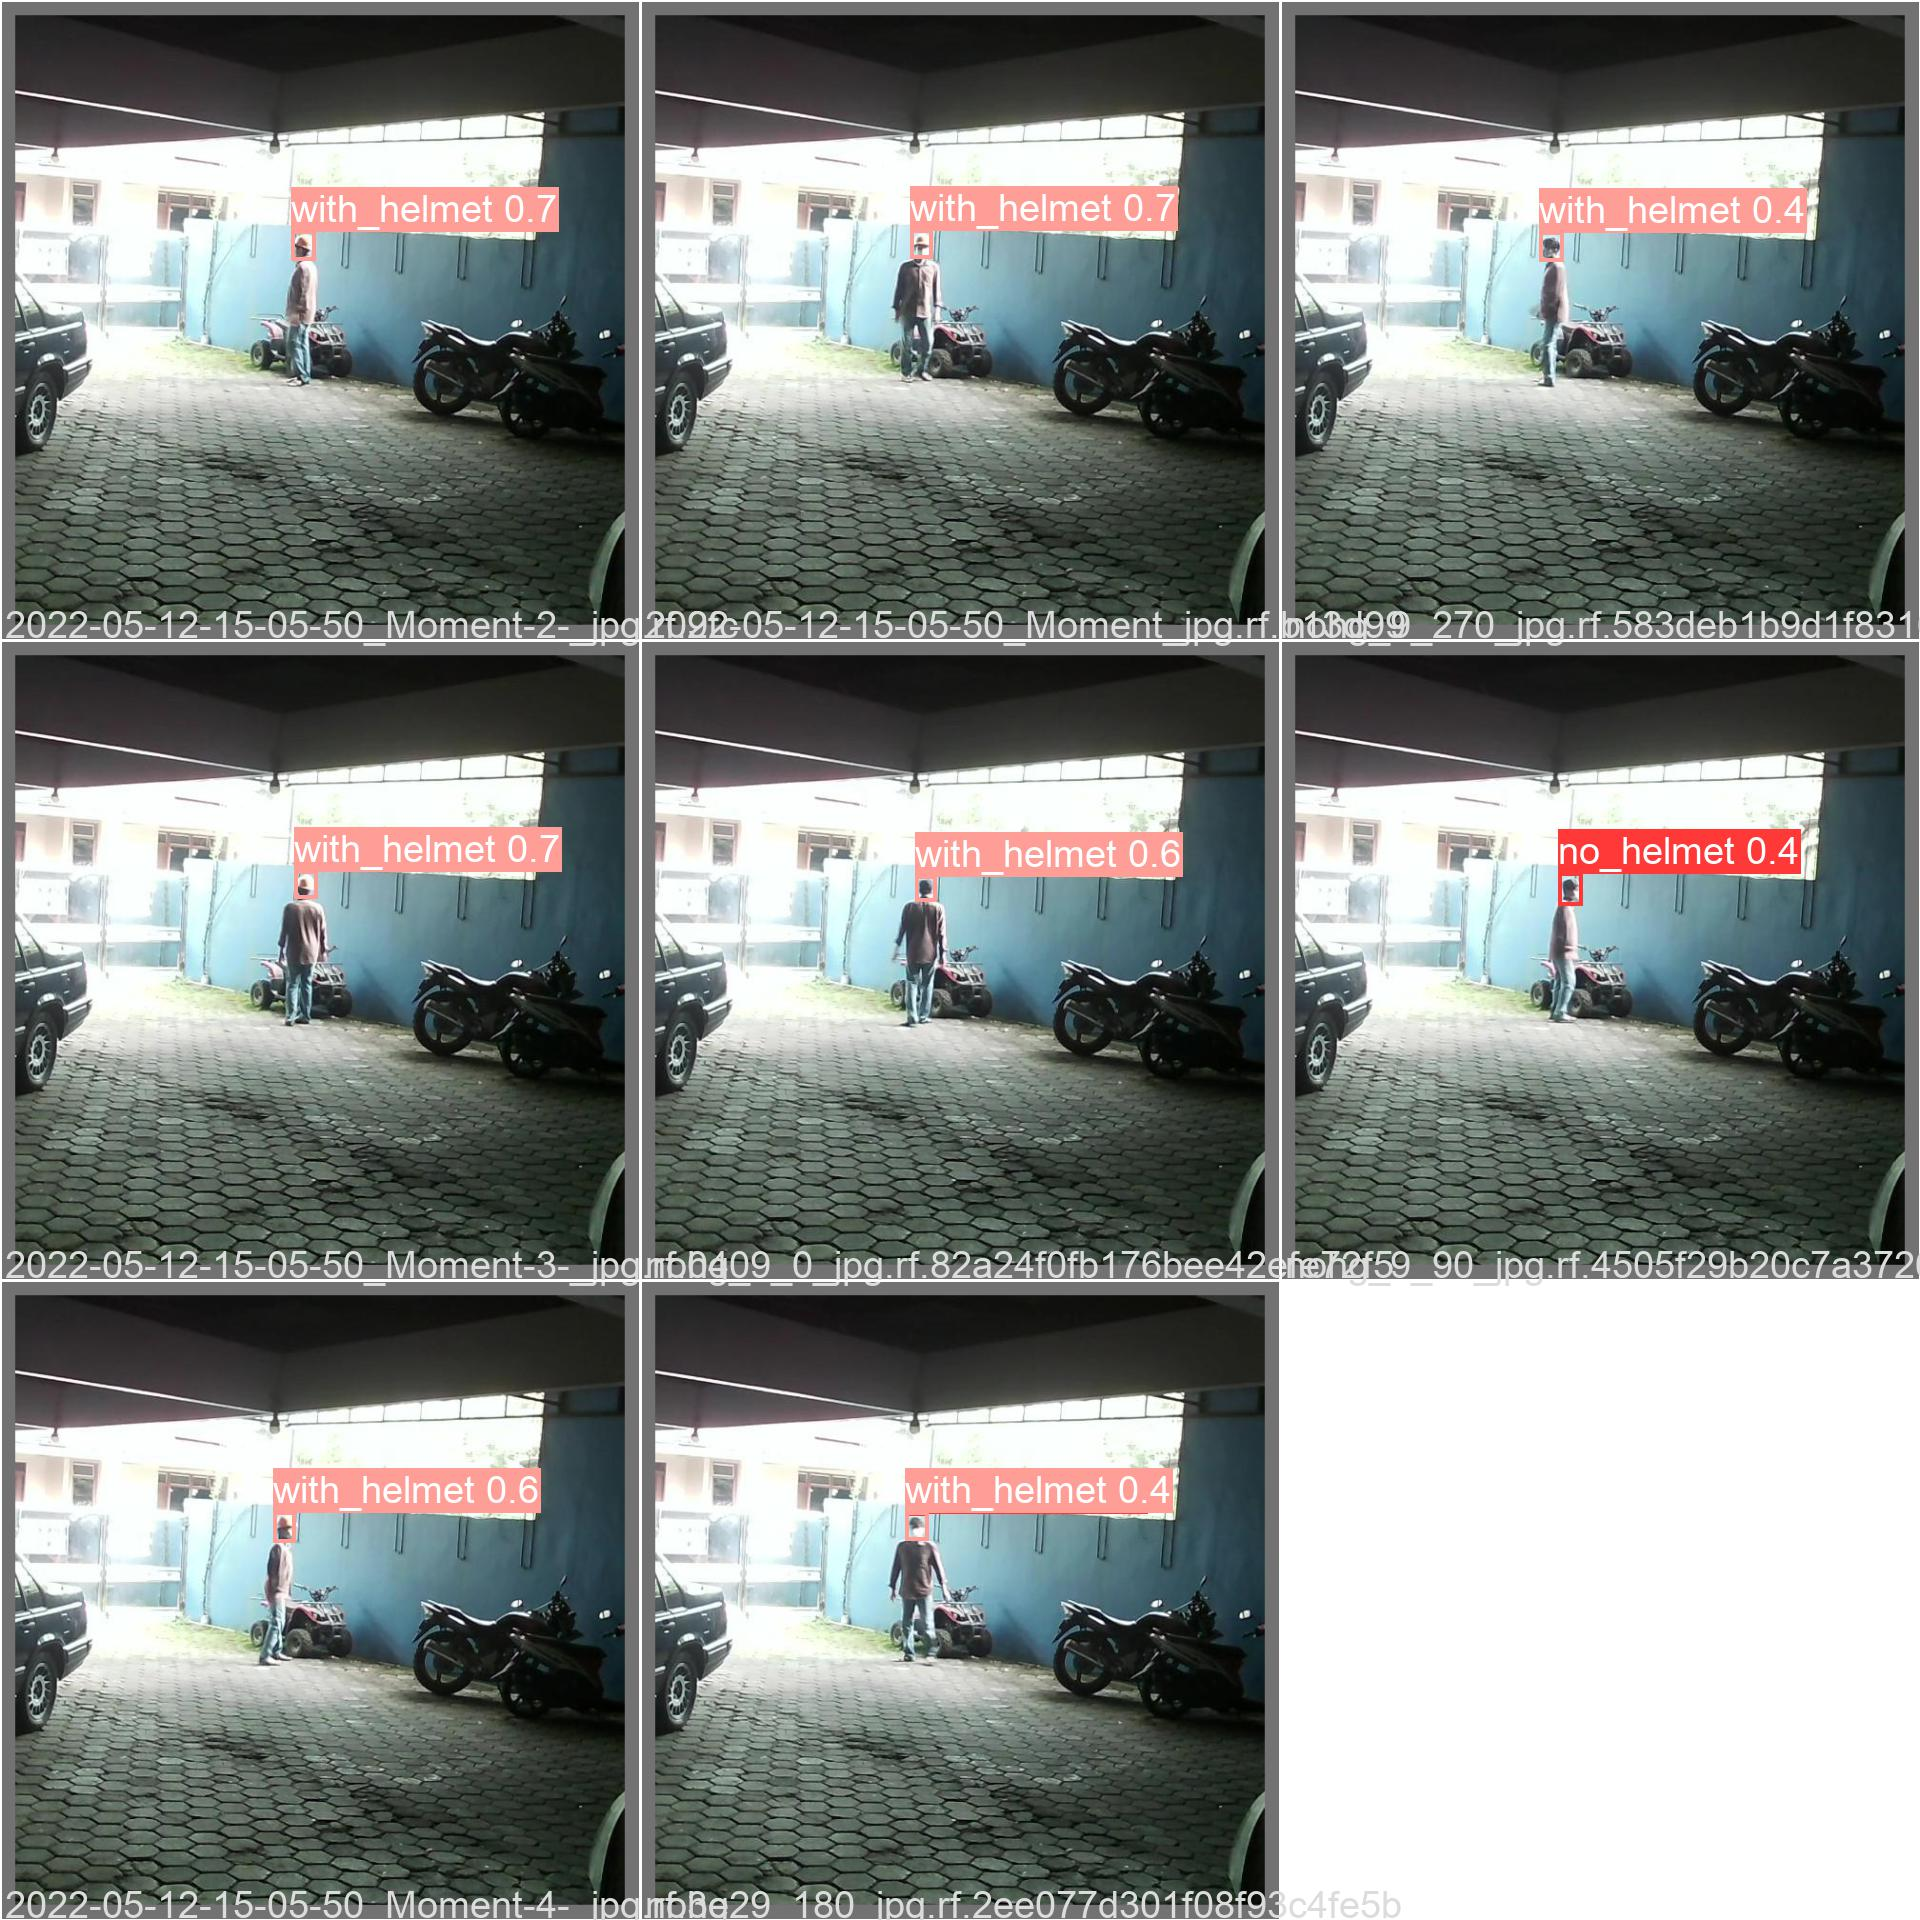
\includegraphics[width=0.31\textwidth]{gambar/BerdasarkanJarak_v2/val_hedec_pure_S/Jarak9/val_batch0_pred.jpg}
    \caption{Hasil Prediksi Untuk Bobot "hedec\_pure\_S" Pada Perbedaan Jarak}
    \label{fig:valjarak_sample_hedec_pure_S}  
  \end{figure}

  \FloatBarrier

  \item \textbf{hedec\_pure\_M}
  
  \par Berikut merupakan hasil validasi pada pengujian prediksi dari jarak 1.3 meter hingga 9 meter untuk bobot "hedec\_pure\_M"
  yang konfigurasi nya menyerupai konfigurasi varian bobot YOLOv5m dari repo YOLOv5 tetapi tidak di-\emph{train} menggunakan bobot \emph{pretrain}-nya.
  Pada Gambar~\ref{fig:grafvaljarak_hedec_pure_M} dapat dilihat bahwa untuk rata-rata kedua kelas dari jarak 1.3 meter hingga 6.7 meter
  memiliki nilai \emph{precision} di atas 0.9, \emph{recall} di atas 0.7 dan mAP 0.995. Tetapi pada jarak 9 meter terjadi penurunan
  nilai \emph{precision} untuk kelas "with\_helmet" mencapai nilai 0.508 dimana terdapat seperti pada umumnya mengalami penurunan. 
  Tabel untuk hasil validasi dari "hedec\_pure\_M" bisa dilihat
  pada Tabel~\ref{tb:hasiljarak_hedec_pure_M}.
  
  \begin{longtable}{|c|c|c|c|c|}
    \caption{Hasil Validasi Perbedaan Jarak Pada \textbf{"hedec\_pure\_M"}}
    \label{tb:hasiljarak_hedec_pure_M}\\
    \hline
    % \rowcolor[HTML]{C0C0C0}
    Jarak     & class        & precision & recall & mAP    \\
    \hline
    1.3 meter & all          & 0.909     & 0.869  & 0.995  \\
    2.6 meter & all          & 0.988     & 1      & 0.995  \\
    4 meter   & all          & 0.978     & 1      & 0.995  \\
    5.3 meter & all          & 0.967     & 1      & 0.995  \\
    6.7 meter & all          & 0.948     & 1      & 0.995  \\
    9 meter   & all          & 0.745     & 1      & 0.97   \\
    1.3 meter & no\_helmet   & 1         & 0.739  & 0.995  \\
    2.6 meter & no\_helmet   & 0.989     & 1      & 0.995  \\
    4 meter   & no\_helmet   & 0.991     & 1      & 0.995  \\
    5.3 meter & no\_helmet   & 0.987     & 1      & 0.995  \\
    6.7 meter & no\_helmet   & 0.994     & 1      & 0.995  \\
    9 meter   & no\_helmet   & 0.981     & 1      & 0.995  \\
    1.3 meter & with\_helmet & 0.818     & 1      & 0.995  \\
    2.6 meter & with\_helmet & 0.988     & 1      & 0.995  \\
    4 meter   & with\_helmet & 0.965     & 1      & 0.995  \\
    5.3 meter & with\_helmet & 0.946     & 1      & 0.995  \\
    6.7 meter & with\_helmet & 0.901     & 1      & 0.995  \\
    9 meter   & with\_helmet & 0.508     & 1      & 0.945  \\
    \hline
  \end{longtable}

  \begin{figure} [h!]
    \centering
    \includegraphics[width=1\textwidth]{gambar/BerdasarkanJarak/hedec_pure_M.png}
    \caption{Grafik \emph{Precision, Recall, mAP} untuk \textbf{"hedec\_pure\_M"} Pada Jarak 1.3 meter Hingga 9 meter}
    \label{fig:grafvaljarak_hedec_pure_M}  
  \end{figure}

  \begin{figure} [h!]
    \centering
    \includegraphics[width=0.25\textwidth]{gambar/BerdasarkanJarak_v2/val_hedec_pure_M/Jarak1_3/val_batch0_pred.jpg}
    \includegraphics[width=0.25\textwidth]{gambar/BerdasarkanJarak_v2/val_hedec_pure_M/Jarak5_3/val_batch0_pred.jpg}
    \includegraphics[width=0.25\textwidth]{gambar/BerdasarkanJarak_v2/val_hedec_pure_M/Jarak9/val_batch0_pred.jpg}
    \caption{Hasil Prediksi Untuk Bobot "hedec\_pure\_M" Pada Perbedaan Jarak}
    \label{fig:valjarak_sample_hedec_pure_M}  
  \end{figure}

   \newpage
  \item \textbf{hedec\_pure\_L}
  
  \par Pada pengujian pada jarak berbeda dari 1.3 meter hingga 9 meter untuk bobot "hedec\_pure\_L" yang merupakan bobot hasil \emph{training}
  yang tidak menggunakan \emph{Pretrained Weights} dari repository YOLOv5 tetapi konfigurasinya menyerupai konfigurasi
  varian \emph{Pretrained Weights} varian YOLOv5l memeiliki beberapa poin yang dapat ditarik. 
  Seperti yang bisa dilihat pada Gambar~\ref{fig:grafvaljarak_hedec_pure_L},
  pada jarak 1.3 meter memiliki nilai yang sedikit rendah untuk \emph{precision, recall} (0.842 dan 0.871) jika dibandingkan dengan jarak 2.6 meter hingga 6.7 meter. 
  Lalu \emph{precision} untuk kelas "with\_helmet" mengalami penurunan drastis pada jarak 9 meter yaitu 0.598.
  Tidak seperti untuk bobot sebandingnya yaitu "hedec\_pretain\_L" yang memiliki hasil validasi yang semua berada di atas 0.9, bobot "hedec\_pure\_L" memiliki penurunan
  pada jarak 9 meter.
  Tabel untuk hasil validasi dari "hedec\_pure\_L" bisa dilihat
  pada Tabel~\ref{tb:hasiljarak_hedec_pure_L}.
  
  \begin{longtable}{|l|l|l|l|l|} 
    \caption{Hasil Validasi Perbedaan Jarak Pada \textbf{"hedec\_pure\_L"}}
    \label{tb:hasiljarak_hedec_pure_L}\\
    \hline
    Jarak     & class        & precision & recall & mAP    \\ 
    \hline
    1.3 meter & all          & 0.842     & 0.871  & 0.978  \\
    2.6 meter & all          & 0.98      & 1      & 0.995  \\
    4 meter   & all          & 0.977     & 1      & 0.995  \\
    5.3 meter & all          & 0.874     & 0.99   & 0.995  \\
    6.7 meter & all          & 0.972     & 1      & 0.995  \\
    9 meter   & all          & 0.794     & 0.849  & 0.995  \\
    1.3 meter & no\_helmet   & 1         & 0.741  & 0.962  \\
    2.6 meter & no\_helmet   & 0.988     & 1      & 0.995  \\
    4 meter   & no\_helmet   & 0.99      & 1      & 0.995  \\
    5.3 meter & no\_helmet   & 1         & 0.98   & 0.995  \\
    6.7 meter & no\_helmet   & 0.987     & 1      & 0.995  \\
    9 meter   & no\_helmet   & 1         & 0.698  & 0.995  \\
    1.3 meter & with\_helmet & 0.683     & 1      & 0.995  \\
    2.6 meter & with\_helmet & 0.971     & 1      & 0.995  \\
    4 meter   & with\_helmet & 0.964     & 1      & 0.995  \\
    5.3 meter & with\_helmet & 0.749     & 1      & 0.995  \\
    6.7 meter & with\_helmet & 0.956     & 1      & 0.995  \\
    9 meter   & with\_helmet & 0.589     & 1      & 0.995  \\
    \hline
  \end{longtable}

  \newpage
  \begin{figure} [h!]
    \centering
    \includegraphics[width=1\textwidth]{gambar/BerdasarkanJarak/hedec_pure_L.png}
    \caption{Grafik \emph{Precision, Recall, mAP} untuk \textbf{"hedec\_pure\_L"} Pada Jarak 1.3 meter Hingga 9 meter}
    \label{fig:grafvaljarak_hedec_pure_L}  
  \end{figure}

  \begin{figure} [h!]
    \centering
    \includegraphics[width=0.31\textwidth]{gambar/BerdasarkanJarak_v2/val_hedec_pure_L/Jarak1_3/val_batch0_pred.jpg}
    \includegraphics[width=0.31\textwidth]{gambar/BerdasarkanJarak_v2/val_hedec_pure_L/Jarak5_3/val_batch0_pred.jpg}
    \includegraphics[width=0.31\textwidth]{gambar/BerdasarkanJarak_v2/val_hedec_pure_L/Jarak9/val_batch0_pred.jpg}
    \caption{Hasil Prediksi Untuk Bobot "hedec\_pure\_L" Pada Perbedaan Jarak}
    \label{fig:valjarak_sample_hedec_pure_L}  
  \end{figure}



\end{enumerate}



% \newpage
\newpage
\section{Pengujian Pada Tingkat Kecerahan Rendah}
\label{sec:pengujianberdasarkantingkatkeceharan}

\par Bagian ini memaparkan performa model melakukan
deteksi pada input gambar dengan tingkat kecerahan rendah. Data validasi berisi
35 gambar dengan jumlah label \emph{no\textunderscore helmet} 20 dan label \emph{with\textunderscore helmet} 57.
Validasi dilakukan pada bobot hasil training yang menggunakan \textit{pretrained weight} dan yang tanpa menggunakan \textit{pretrained weight}. 

\subsection{Pengujian Pada Tingkat Kecerahan Rendah dengan \emph{Pretrained Weight}}
\label{subsec:lowlight_pretrained}

\par Berikut merupakan pemaparan hasil validasi pada data validasi menggunakan \emph{weight} yang di-\emph{train} menggunakan
\emph{pretrained weights} yang disedikan repo YOLOv5 yang selanjutnya disebut sebagai "hedec\textunderscore pretain". 
Seperti yang dijelaskan pada Subbab~\ref{subsec:ujiperforma_coco}. 


\begin{enumerate}
  \item \textbf{hedec\textunderscore pretrain\textunderscore N}
  
  \par Dilakukan pengujian kecerahan rendah dengan menggunakan bobot yang di-\emph{train} menggunakan bobot
  pretrain COCO untuk varian \emph{nano} yang merupakan varian paling kecil dari semua bobot yang disediakan 
  dari repo. Didapatkan rata - rata presisi untuk semua kelas 0.767 dan \emph{recall} untuk semua kelas 0.373.
  \par Didapati untuk kelas \emph{no\textunderscore helmet} mendapatkan nilai \emph{precision} 1 dan \emph{recall}
  0. Hal ini dikarenakan objek kepala tanpa menggunakan helm tidak ada yang terdektsi dan atau terdeteksi
  sebagai kelas \emph{with\textunderscore helmet}. 
  
  \begin{longtable}{|c|c|c|c|}
    \caption{Hasil Validasi Pada Tingkat Kecerahan Rendah dengan hedec\textunderscore pretrain\textunderscore N   }
    \label{tb:validasitingkatacerahrendah_yolo5n}\\
    \hline
    % \rowcolor[HTML]{C0C0C0}
    \textbf{\emph{Class} }                     & \textbf{\emph{Precision}}  & \textbf{\emph{Recall}} & \textbf{\emph{mAP@.5}}\\
    \hline
    all                                                 & 0.767          & 0.373        & 0.415         \\
    no\textunderscore helmet                            & 1              & 0            & 0.143          \\
    with\textunderscore helmet                          & 0.534          & 0.745        & 0.687         \\
    \hline
  \end{longtable}
  
  \begin{figure}[h]
    \centering
    \includegraphics[scale=0.2]{gambar/train_v2_val/low_ligjt/yolonano/val_batch0_pred.jpg}
    % \includegraphics[scale=0.1]{gambar/train_v2_val/low_ligjt/yolonano/val_batch0_labels.jpg}
    \caption{Hasil Prediksi Pada Keadaan Rendah dengan hedec\textunderscore pretrain\textunderscore N    }
    % \label{fig:labelbaru}  
  \end{figure}

  \FloatBarrier
   
  \item \textbf{hedec\textunderscore pretrain\textunderscore S}
  
  \par Dilakukan pengujian kecerahan rendah dengan menggunakan bobot yang di-\emph{train} menggunakan bobot
  pretrain COCO untuk varian \emph{small}. Didapatkan rata - rata presisi untuk semua kelas 0.775 dan \emph{recall} untuk semua
  kelas 0.799. Terdapat beberapa \emph{False Positive} dalam prediksi yaitu helm motor yang diletakkan diatas
  motor diprediksi sebagai \emph{with\textunderscore helmet} begitu juga.
  
  \begin{longtable}{|c|c|c|c|}
    \caption{Hasil Validasi Pada Tingkat Kecerahan Rendah dengan hedec\textunderscore pretrain\textunderscore S}
    \label{tb:validasitingkatacerahrendah_yolov5s}\\
    \hline
    % \rowcolor[HTML]{C0C0C0}
    \textbf{\emph{Class} }                     & \textbf{\emph{Precision}}  & \textbf{\emph{Recall}} & \textbf{\emph{mAP@.5}}\\
    \hline
    all                                                 & 0.775          & 0.799        & 0.823         \\
    no\textunderscore helmet                            & 0.862           & 0.65        & 0.713          \\
    with\textunderscore helmet                          & 0.689           & 0.947        & 0.933         \\
    \hline
  \end{longtable}

  \newpage
  \begin{figure} [h!]
    \centering
    \includegraphics[scale=0.2]{gambar/train_v2_val/low_ligjt/yolosmall/low_light_val_batch0_pred.jpg}
    % \includegraphics[scale=0.1]{gambar/train_v2_val/low_ligjt/yolosmall/lowlight_val_batch0_labels.jpg}
    \caption{Hasil Prediksi Pada Keadaan dengan hedec\textunderscore pretrain\textunderscore S}
    % \label{fig:labelbaru}  
  \end{figure}


  
  \item \textbf{hedec\textunderscore pretrain\textunderscore M} 
  
  \par Dilakukan pengujian kecerahan rendah dengan menggunakan bobot yang di-\emph{train} menggunakan bobot
  pretrain COCO untuk varian \emph{medium}. Didapatkan rata - rata presisi untuk semua kelas 0.833 dan \emph{recall} untuk semua
  kelas 0.831. Didapati hasil \emph{precision} dan \emph{recall} untuk kelas \emph{no\textunderscore helm} ,yang biasanya
  memiliki nilai yang kurang bagus pada varian bobot nano , mendapatkan nilai 1 dan 0.68 yang dimana lebih bagus. 
  Varian Medium ini merupakan varian yang memiliki hasil validasi paling tinggi untuk \emph{precision} dan \emph{recall} nya diantara semua \emph{weight}
  yang di \emph{train} menggunakan \emph{pretrained weights} dari YOLOv5 bahkan melebihi varian YOLOv5l yang akan dipaparkan di bagian selanjutnya.
  \newpage
  \begin{longtable}{|c|c|c|c|}
    \caption{Hasil Validasi Pada Tingkat Kecerahan Rendah dengan hedec\textunderscore pretrain\textunderscore M}
    \label{tb:validasitingkatacerahrendah_yolov5m}\\
    \hline
    % \rowcolor[HTML]{C0C0C0}
    \textbf{\emph{Class} }                     & \textbf{\emph{Precision}}  & \textbf{\emph{Recall}} & \textbf{\emph{mAP@.5}}\\
    \hline
    all                                                 & 0.833          & 0.831       & 0.893         \\
    no\textunderscore helmet                            & 1              & 0.68        & 0.814         \\
    with\textunderscore helmet                          & 0.666          & 0.982       & 0.973         \\
    \hline
  \end{longtable}

  
  \begin{figure} [h!]
    \centering
    \includegraphics[scale=0.2]{gambar/train_v2_val/low_ligjt/yolomedium/val_batch0_pred.jpg}
    % \includegraphics[scale=0.1]{gambar/train_v2_val/low_ligjt/yolomedium/val_batch0_labels.jpg}
    \caption{Hasil Prediksi Pada Keadaan dengan hedec\textunderscore pretrain\textunderscore M}
    % \label{fig:labelbaru}  
  \end{figure}


  \item \textbf{hedec\textunderscore pretrain\textunderscore L}
  
  \par Dilakukan pengujian kecerahan rendah dengan menggunakan bobot yang di-\emph{train} menggunakan bobot
  pretrain COCO untuk varian \emph{large}. Didapatkan rata - rata presisi untuk semua kelas 0.811 dan \emph{recall} untuk semua
  kelas 0.765 dimana lebih kecil dibandingkan varian \emph{medium}. Didapati juga hasil \emph{precision} dan \emph{recall} untuk kelas \emph{no\textunderscore helm} yang mengalami penurunan dibanding
  menggunakan variant \emph{medium} yaitu 0.914 untuk \emph{precision} dan 0.6 untuk \emph{recall}. Selain itu untuk
  \emph{inference time} nya tentu saja mengalami kenaikan dibandingan dengan varian - varian sebelumnya yang lebih kecil.
  
  \begin{longtable}{|c|c|c|c|}
    \caption{Hasil Validasi Pada Tingkat Kecerahan Rendah dengan hedec\textunderscore pretrain\textunderscore L}
    \label{tb:validasitingkatacerahrendah_yolov5l}\\
    \hline
    % \rowcolor[HTML]{C0C0C0}
    \textbf{\emph{Class} }                     & \textbf{\emph{Precision}}  & \textbf{\emph{Recall}} & \textbf{\emph{mAP@.5}}\\
    \hline
    all                                                 & 0.811          & 0.765       & 0.893         \\
    no\textunderscore helmet                            & 0.914          & 0.6         & 0.724         \\
    with\textunderscore helmet                          & 0.708          & 0.93        & 0.931         \\
    \hline
  \end{longtable}
  
  \begin{figure} [h!]
    \centering
    \includegraphics[scale=0.2]{gambar/train_v2_val/low_ligjt/yololarge/val_batch0_pred.jpg}
    % \includegraphics[scale=0.1]{gambar/train_v2_val/low_ligjt/yololarge/val_batch0_labels.jpg}
    \caption{Hasil Prediksi Pada Keadaan dengan hedec\textunderscore pretrain\textunderscore Ll}
    % \label{fig:labelbaru}  
  \end{figure}

\end{enumerate}


\subsection{Pengujian Pada Tingkat Kecerahan Rendah dengan \emph{Weight} Murni Deteksi Helm Keselamatan Kerja}
\label{subsec:lowlight_pure}

\par Berikut merupakan pemaparan hasil validasi menggunakan data validasi pada keadaan minim pencahayaan menggunakan
\emph{weight} yang merupakan hasil \emph{train} dari dataset Deteksi Helm Keselamatan Kerja tanpa menggunakan \emph{pretrained weight}.
Hasil \emph{train} tanpa menggunakan \emph{pretrain weight} ini selanjutkan akan disebut sebagai "hedec\textunderscore pure".

 

\begin{enumerate}
  \newpage
  \item \textbf{hedec\textunderscore pure\textunderscore N } 
  
  \par Dilakukan pengujian kecerahan rendah dengan menggunakan bobot yang di-\emph{train} tanpa menggunakan bobot
  pretrain COCO tetapi konfigurasi modelnya dibuat serupa dengan konfigurasi YOLOv5n. 
  Didapatkan rata - rata presisi untuk semua kelas 0.659   dan \emph{recall} untuk semuakelas 0.696.
  \par  Sewajarnya varian ini mendapatkan nilai \emph{precision} dan \emph{recall} paling kecl diantara varian lainnya dan juga \emph{inference speed}
  yang paling cepat dibanding varian lainnya pada \emph{weight} murni \emph{tanpa pretrained weight}.
  
  \begin{longtable}{|c|c|c|c|}
    \caption{Hasil Validasi Pada Tingkat Kecerahan Rendah dengan \emph{Hedec Nano}}
    \label{tb:validasitingkatacerahrendah_hedecN}\\
    \hline
    % \rowcolor[HTML]{C0C0C0}
    \textbf{\emph{Class} }                     & \textbf{\emph{Precision}}  & \textbf{\emph{Recall}} & \textbf{\emph{mAP@.5}}\\
    \hline
    all                                                 & 0.659          & 0.696        & 0.731         \\
    no\textunderscore helmet                            & 0.76           & 0.55         & 0.621         \\
    with\textunderscore helmet                          & 0.558          & 0.842        & 0.842         \\
    \hline
  \end{longtable}
  
  \begin{figure}[h]
    \centering
    \includegraphics[scale=0.2]{gambar/train_v2_val/low_ligjt/customNano/val_batch0_pred.jpg}
    % \includegraphics[scale=0.1]{gambar/train_v2_val/low_ligjt/customNano/val_batch0_labels.jpg}
    \caption{Hasil Prediksi Pada Keadaan dengan \emph{Weight Hedec Nano}}
    % \label{fig:labelbaru}  
  \end{figure}
  
  
  \item \textbf{hedec\textunderscore pure\textunderscore S }
  
  \par Dilakukan pengujian kecerahan rendah dengan menggunakan bobot yang di-\emph{train} tanpa menggunakan bobot
  pretrain COCO tetapi konfigurasi modelnya dibuat serupa dengan konfigurasi YOLOv5s. 
  Didapatkan rata - rata presisi untuk semua kelas 0.706   dan \emph{recall} untuk semuakelas 0.696 dimana sedikit lebih baik
  dibandingkan varian \emph{Nano} sebelumnya.
  
  \begin{longtable}{|c|c|c|c|}
    \caption{Hasil Validasi Pada Tingkat Kecerahan Rendah dengan \emph{Hedec Small}}
    \label{tb:validasitingkatacerahrendah_hedecS}\\
    \hline
    % \rowcolor[HTML]{C0C0C0}
    \textbf{\emph{Class} }                     & \textbf{\emph{Precision}}  & \textbf{\emph{Recall}} & \textbf{\emph{mAP@.5}}\\
    \hline
    all                                                 & 0.706          & 0.696        & 0.847         \\
    no\textunderscore helmet                            & 0.885          & 0.771        & 0.789         \\
    with\textunderscore helmet                          & 0.623          & 0.947        & 0.905         \\
    \hline
  \end{longtable}
  
  \begin{figure} [h!]
    \centering
    \includegraphics[scale=0.2]{gambar/train_v2_val/low_ligjt/customSmall/val_batch0_pred.jpg}
    % \includegraphics[scale=0.1]{gambar/train_v2_val/low_ligjt/customSmall/val_batch0_labels.jpg}
    \caption{Hasil Prediksi Pada Keadaan dengan \emph{Weight Hedec Small}}
    % \label{fig:labelbaru}  
  \end{figure}

   \newpage
  \item \textbf{hedec\textunderscore pure\textunderscore M }
  
  \par Dilakukan pengujian kecerahan rendah dengan menggunakan bobot yang di-\emph{train} tanpa menggunakan bobot
  pretrain COCO tetapi konfigurasi modelnya dibuat serupa dengan konfigurasi YOLOv5m. 
  Didapatkan rata - rata presisi untuk semua kelas 0.731   dan \emph{recall} untuk semuakelas 0.862 dimana lebih baik dibandingkan
  varian \emph{Small}.
  
  \begin{longtable}{|c|c|c|c|}
    \caption{Hasil Validasi Pada Tingkat Kecerahan Rendah dengan \emph{Hedec Medium}}
    \label{tb:validasitingkatacerahrendah_hedecM}\\
    \hline
    % \rowcolor[HTML]{C0C0C0}
    \textbf{\emph{Class} }                     & \textbf{\emph{Precision}}  & \textbf{\emph{Recall}} & \textbf{\emph{mAP@.5}}\\
    \hline
    all                                                 & 0.731          & 0.862       & 0.827         \\
    no\textunderscore helmet                            & 0.799          & 0.793       & 0.757         \\
    with\textunderscore helmet                          & 0.663          & 0.93        & 0.897         \\
    \hline
  \end{longtable}
  
  \begin{figure} [h!]
    \centering
    \includegraphics[scale=0.2]{gambar/train_v2_val/low_ligjt/customMedium/val_batch0_pred.jpg}
    % \includegraphics[scale=0.1]{gambar/train_v2_val/low_ligjt/customMedium/val_batch0_labels.jpg}
    \caption{Hasil Prediksi Pada Keadaan dengan \emph{Weight Hedec Medium}}
    % \label{fig:labelbaru}  
  \end{figure}
  
  \newpage
  \item \textbf{hedec\textunderscore pure\textunderscore L }
  \par Dilakukan pengujian kecerahan rendah dengan menggunakan bobot yang di-\emph{train} tanpa menggunakan bobot
  pretrain COCO tetapi konfigurasi modelnya dibuat serupa dengan konfigurasi YOLOv5l. 
  Didapatkan rata - rata presisi untuk semua kelas 0.743   dan \emph{recall} untuk semuakelas 0.755.
  \par Berbeda dengan bobot imbangan variasi \emph{Large} yang dilatih menggunakan Pretrained COCO, \emph{overall precision} pada varian ini
  sedikit lebih baik daripada varian \emph{Medium} nya, tetapi untuk \emph{Recall} sama - sama lebih kecil.
  
   
  \begin{longtable}{|c|c|c|c|}
    \caption{Hasil Validasi Pada Tingkat Kecerahan Rendah dengan \emph{Hedec Large}}
    \label{tb:validasitingkatacerahrendah_hedecL}\\
    \hline
    % \rowcolor[HTML]{C0C0C0}
    \textbf{\emph{Class} }                     & \textbf{\emph{Precision}}  & \textbf{\emph{Recall}} & \textbf{\emph{mAP@.5}}\\
    \hline
    all                                                 & 0.743          & 0.755       & 0.789         \\
    no\textunderscore helmet                            & 0.85           & 0.65        & 0.733         \\
    with\textunderscore helmet                          & 0.663          & 0.86        & 0.845         \\
    \hline
  \end{longtable}
  
  \begin{figure} [h!]
    \centering
    \includegraphics[width=0.8\textwidth]{gambar/train_v2_val/low_ligjt/customLarge/val_batch0_pred.jpg}
    % \includegraphics[scale=0.1]{gambar/train_v2_val/low_ligjt/customLarge/val_batch0_labels.jpg}
    \caption{Hasil Prediksi Pada Keadaan dengan \emph{Weight Hedec Large}}
    % \label{fig:labelbaru}  
  \end{figure}
  
\end{enumerate}

\subsection{Analisis Pengujian Pada Pencahayaan Rendah}
  \label{subsec:analisis_lowlight}

  \begin{figure} [h!]
    \centering
    \includegraphics[width=1.0\textwidth]{gambar/lowlight_grafic/Low Light - all.png}
    \caption{Grafik Hasil Testing Pada Pencahayaan Rendah untuk Semua Kelas}
    \label{fig:graf_lowlight_all}  
  \end{figure}

  \begin{figure} [h!]
    \centering
    \includegraphics[width=.45\textwidth]{gambar/lowlight_grafic/Low Light - no_helmet.png}
    \includegraphics[width=.45\textwidth]{gambar/lowlight_grafic/Low Light - with_helmet.png}
    \caption{Grafik Hasil Testing Pada Pencahayaan Rendah untuk Masing - Masing Kelas}
    \label{fig:graf_lowlight_eachclass}  
  \end{figure}

  \par Berdasarkan hasil yang sudah diaparkan untuk bobot varian hasil 
  pretrain dan murni tanpa pretrain yang diapaprkan pada Subbab~\ref{subsec:lowlight_pretrained} 
  dan Subbab~\ref{subsec:lowlight_pure}, dapat ditarik beberapa point. Varian bobot "hedec\_pretrain\_N"
  memiliki nilai \emph{recall} paling rendah dari semua bobot dikarenakan kegagalan dalam mendeteksi
  kelas "no\_helmet" pada dataset testing yang disediakan. Secara umum, bobot yang paling bagus digunakan
  pada kasus pencahayaan rendah terdapat pada bobot "hedec\_pretrain\_L" yang merupakan
  bobot yang dilatih menggunakan\emph{pretrained weights}" untuk varian yolov5l yang memiliki
  \emph{"depth\_multiplier"} dan "\emph{width\_multiplier}" paling besar. Selain itu, seperti yang
  ditunjukkan pada Gambar~\ref{fig:graf_lowlight_all} untuk varian yang menggunakan
  \emph{pretrained weights} jika diurutkan dari varian \emph{Nano} hingga \emph{Large} selalu mengalami
  kenaikan nilai mAP.5 nya. Tetapi untuk varian yang dilatih murni hanya menggunakan Dataset Helm Keselamatan Kerja
  mengalami kenaikan nilai mAP.5 hanya sampai pada varian \emph{Small (S)} dan setelah itu mengalami penurunan hingga varian \emph{Large (L)}.



\section{Pengujian Model YOLOv5 dengan \emph{Helmet Detection Weights} Pada Jetson Nano}
\label{sec:jetsonnano_hedectest}

\par Bagian ini merupakan pemaparan hasil pengujian performa Model YOLOv5 dengan bobot - bobot yang sudah di\emph{train}
sebelumnya pada Jetson Nano. Tujuan dari pengujian ini yaitu membandingkan effektifitas dari masing - masing
bobot yang sudah dibuat pada aspek performa \emph{inference} mengingat Jetson Nano merupakan \emph{mini-computer} yang memiliki
\emph{Graphic Processing Unit}(GPU)nya sendiri dan memang didesain untuk aplikasi AI IoT. Pengujuran yang diambil pada pengujian ini
yaitu nilai \emph{Frame Per Second}(FPS).

 
\par Pengujian dilakukan menggunakan Webcam Nemesis NYK A-90 Everest yang dipasang dengan Jetson Nano melalui kabel USB. 
Pengujian dilakukan pada resolusi 256, 480, dan 640. Hasil pengukuran FPS pada pengujian YOLOv5 Helmet Detection dipaparkan pada Tabel~\ref{tb:jetsonanoperformancetest}.



\begin{longtable}{|l|l|l|l|} 
  \caption{Hasil Test Peforma Pad Jetson Nano}
  \label{tb:jetsonanoperformancetest}\\
  \hline
  \multirow{2}{*}{\textbf{Nama Bobot}} & \multicolumn{3}{l|}{\textbf{Resolusi}}      \\ 
  \cline{2-4}
                                       & \textbf{256} & \textbf{480} & \textbf{640}  \\ 
  \hline
  hedec\_pretrain\_N                   & 24.4         & 22           & 18.5          \\
  hedec\_pretrain\_S                   & 22.2         & 13           & 7.8           \\
  hedec\_pretrain\_M                   & 15.2         & 5.7          & 3.4           \\
  hedec\_pretrain\_L                   & 8            & 3.2          & 1.8           \\
  hedec\_pure\_N                       & 24.9         & 21.5         & 18.4          \\
  hedec\_pure\_S                       & 23           & 12.3         & 7.8           \\
  hedec\_pure\_M                       & 15           & 5.4          & 3.3           \\
  hedec\_pure\_L                       & 8.3          & 3            & 1.8           \\
  \hline
\end{longtable}

\begin{figure} [h!]
  \centering
  \includegraphics[width=.45\textwidth]{gambar/performance_jetson/Frame Rate Hedec_Pretrain di Jetson Nano.png}
  \includegraphics[width=.45\textwidth]{gambar/performance_jetson/Frame Rate Hedec_Puredi Jetson Nano.png}
  \caption{Grafik Performa berdasarkan Frame Rate Pada Jetson Nano Untuk "Hedec\_pretrain" dan "Hedec\_pure"}
  \label{fig:graf_jetsonano}  
\end{figure}

\FloatBarrier

\par Berdasarkan hasil pengujian pada ~\ref{tb:jetsonanoperformancetest}, terdapat beberapa poin analisis yang bisa diambil.
Performa dari nilai \emph{Frame Rate} dari \emph{weight} yang menggunakan \emph{Pretrained Weights} dengan pasangan bandingnya di \emph{weight}
yang tidak menggunakan \emph{Pretrained Weights} memiliki performa yang tidak berbeda jauh. Sewajarnya, varian \emph{Nano (N)} dari
\emph{Pretrained Weight} atau \emph{Pure Weight} memiliki FPS paling tinggi dibandingkan varian diatasnya yaitu S,M,dan L.

\section{Pengujian Sistem dan Model Pada \emph{Headgear} Lain}
\label{sec:otherheadgear_test}

\par Pada bagian ini dilakukan pengujian pada \emph{headgear} selain helm keselamatan kerja yaitu topi dan beberapa \emph{headgear} lainnya. Terdapat kemungkinan pada area pekerjaan terdapat pekerja lapangan yang menggunakan \emph{headgear} selain helm keselamatan kerja seperti topi. Tetapi pelindung kepala selain helm keselamatan kerja berada diluar batasan masalah yang dibahas pada Subbab~\ref{sec:batasanmasalah}.

Dilakukan 138 kali pengambilan test untuk \emph{headgear} selain helm keselamatan kerja, dengan confidence\_threshold 0.25 dan iou\_threshold 0.45, didapatkan untuk hasil dari sisi kelas "no\_helmet" sebagai berikut:

\begin{enumerate}[nolistsep]
  \item True Postive : 65
  \item False Positive : 1
  \item False Negative : 66
  \item Precision : 0.9848484848
  \item Recall : 0.4961832061
\end{enumerate}

Diluar dari sisi kelas "no\_helmet", terjadi 63 kali False Positive untuk kelas "with\_helmet" dimana model mendeteksi topi atau headgear lainnya sebagai "with\_helmet".

Lalu berikut merupakan hasil pengujian sistem alarm, hanya terdapat False dan Negative dikarenakan semua test dilakukan pada keadaan dimana seharusnya alarm menyala :

\begin{enumerate}[nolistsep]
  \item True : 66
  \item False : 72
  \item Akurasi : 0.4782608696
\end{enumerate}

Didapati masih sering terjadi False Negative untuk deteksi "no\_helmet" pada penggunaan topi dimana tidak terdektsi sebagai "no\_helmet" atau bahkan terdeteksi sebagai "with\_helmet".

\begin{figure} [h!]
  \centering
  \includegraphics[width=0.3\textwidth]{gambar/pengujian/Screenshot_105.png}
  \includegraphics[width=0.3\textwidth]{gambar/pengujian/Screenshot_106.png}
  \includegraphics[width=0.3\textwidth]{gambar/pengujian/Screenshot_107.png}
  \caption{Pengujian Pada \emph{Headgear} selain Helm Keselamatan Kerja}
  \label{fig:pengujian_headgear}  
\end{figure}


\section{Pengujian Sistem Deteksi Helm Keselamatan Kerja}
\label{sec:system_check}

\par Pada bagian ini akan dipaparkan berbagai macam pengujian terhadap sistem deteksi yang dikembangkan. Seperti yang sebelumnya sudah dijelaskan pada Subab~\ref{sec:perancangansistem}, sistem deteksi helm keselamatan kerja ini akan menjalankan mekanisme alarm berupa suara audio sirine alarm jika dalam frame terdeteksi satu atau lebih kelas "no\_helmet".

\par Pengujian - pengujian sebagian besar dilakukan dengan cara mengambil beberapa sampel gambar dari hasil rekaman sistem di beberapa kondisi berbeda : perbedaan jarak, kecerahan rendah, sudut pandang CCTV, dan percobaan penjalanan di SBC Jetson Nano. Pengujian ini berfokus untuk menjawab pertanyaan "Seberapa akurat sistem menyalakan alarm saat alarm memang dibutuhkan untuk dinyalakan?". Sisi "Positif" akan dilihat dari saat alarm dinyalakan dan "Negatif" saat alarm tidak menyala. 

\subsection{Pengujain Sistem Pada Perbedaan jarak}
\label{subsec:systest_test_dist}

\par Pengujian ini dilakukan dengan pada perbedaan jarak antara kamera dengan objek yang diamati (orang yang memakai atau tidak memakai helm keselamatan kerja). Pengujian dilakukan dengan mengambil beberapa sampel gambar dari rekaman yang menjalankan deteksi pada jarak 1 meter hingga 10 meter.

\begin{table}
    \centering
    \caption{Hasil Pengujain Sistem Pada Perbedaan jarak}
    \label{tb:systest_dist_test}
    \begin{tabular}{|l|l|l|l|l|l|l|} 
    \hline
    Distance & TP & TN & FP & FN & Akurasi    & Jumlah Test  \\ 
    \hline
    1m       & 17 & 61 & 7  & 0  & 0.9176470588 & 85               \\ 
    \hline
    3m       & 20 & 44 & 0  & 2  & 0.9696969697 & 66               \\ 
    \hline
    5m       & 40 & 53 & 0  & 0  & 1            & 93               \\ 
    \hline
    7m       & 32 & 56 & 0  & 0  & 1            & 88               \\ 
    \hline
    10m      & 78 & 32 & 0  & 0  & 1            & 110              \\
    \hline
    \end{tabular}
\end{table}

\par Berdasarkan hasil pengujian yang ditunjukan pada Tabel~\ref{tb:systest_dist_test}, akurasi pada jarak 5 meter hingga 10 meter bernilai 1 karena tidak mengalami kesalahan menyalakan alarm sama sekali dari masing - masing jumlah percobaan seperti yang dapat dilihat pada Gambar~\ref{fig:sys_1-3_meter}. Pada jarak 1 meter dan 3 meter terdapat beberapa \emph{False} dimana pada jarak 1 meter mengalami 7 kali False Positive atau dimana alarm menyala disaat tidak seharusnya menyala dan pada jarak 3 meter terdapat 2 kali False Negative dimana alarm seharusnya menyala tetapi tidak seperti yang dapat dilihat pada Gambar~\ref{fig:sys_5-9_meter}.

\begin{figure} [h]
    \centering
    \includegraphics[width=0.3\textwidth]{gambar/sistem_jarak/1-3_jelek/jarak_helmet_white (21).png}
    \includegraphics[width=0.3\textwidth]{gambar/sistem_jarak/1-3_jelek/jaraknohelmet (1).png}
    \caption{Deteksi Pada Jarak 1 dan 3 meter}
    \label{fig:sys_1-3_meter}  
\end{figure}

\begin{figure} [h]
    \centering
    \includegraphics[width=0.3\textwidth]{gambar/sistem_jarak/5-9_bagus/jarak_helmet_orange (67).png}
    \includegraphics[width=0.3\textwidth]{gambar/sistem_jarak/5-9_bagus/jarak_helmet_white (129).png}
    \includegraphics[width=0.3\textwidth]{gambar/sistem_jarak/5-9_bagus/jaraknohelmet (82).png}
    \caption{Deteksi Pada Jarak 5 - 10 meter}
    \label{fig:sys_5-9_meter}  
\end{figure}



\subsection{Pengujian Pada Sudut Pandang CCTV}
\label{subsec:systest_test_cctv}

\par Pengujian ini dilakukan dengan tujuan mengimitasi bagaimana CCTV biasanya dipasang pada suatu \emph{checkpoint} di lokasi konstruksi yang biasanya dipasang dengan sudut 45 derajat. Hasil pengujian ini ditunjukan pada Tabel~\ref{tb:systest_cctv}.


\begin{table}
    \centering
    \caption{Hasil Pengujian Pada Sudut Pandang CCTV}
    \label{tb:systest_cctv}
    \begin{tabular}{|l|l|l|l|l|} 
    \hline
    TP & TN & FP & FN & Akurasi         \\ 
    \hline
    27 & 28 & 0  & 9  & 0.859375         \\ 
    \hline
    \multicolumn{2}{|l|}{55}   & \multicolumn{2}{l|}{9} & 64 tes \\
    \hline
    \end{tabular}
\end{table}

Berdasarkan hasil pengujian tersebut, dari 64 kali pengambilan sampel untuk pengujian, didapati 9 kali \emph{False Negative} dimana terjadi 9 kali kegagalan menyalakan alarm disaat seharusnya menyalakan alarm. Beberapa contoh kegagalan menyalakan alarm atau False Negative ini dicontohkan seperti Gambar~\ref{fig:sys_cctvori_fn}. Tetapi untuk \emph{True Positive} dan \emph{True Negative} lebih banyak terjadi dengan angka 27 dan 28 kali seperti yang ditunjukkan pada Gambar~\ref{fig:sys_cctvori_fn}.

\begin{figure} [h]
    \centering
    \includegraphics[width=0.3\textwidth]{gambar/sistem_cctvori/betuls/cctv_perspective_pred (7).png}
    \includegraphics[width=0.3\textwidth]{gambar/sistem_cctvori/betuls/cctv_perspective_pred (11).png}
    \includegraphics[width=0.3\textwidth]{gambar/sistem_cctvori/betuls/cctv_perspective_pred (53).png}
    \caption{Sistem Deteksi Tepat Pada Sudut 45 Derajat (CCTV)}
    \label{fig:sys_cctvori_true}  
\end{figure}

\begin{figure} [h]
    \centering
    \includegraphics[width=0.3\textwidth]{gambar/sistem_cctvori/falsenegative/cctv_perspective_pred (73).png}
    \includegraphics[width=0.3\textwidth]{gambar/sistem_cctvori/falsenegative/cctv_perspective_pred (83).png}
    \includegraphics[width=0.3\textwidth]{gambar/sistem_cctvori/falsenegative/cctv_perspective_pred (97).png}
    \caption{Sistem Deteksi \emph{False Negative} Pada Sudut 45 Derajat (CCTV)}
    \label{fig:sys_cctvori_fn}  
\end{figure}


\subsection{Pengujian \emph{Real-Time} Pada Jetson Nano}
\label{subsec:systest_test_jetsonrealtime}

\par Pengujian ini dilakukan dengan memanfaatkan Jetson Nano untuk \emph{deployment} dari sistem deteksi helm keselamatan kerja. Dengan menggunakan camera yang sama dan dipasang dengan sudut yang sama seperti pada Subbab~\ref{subsec:systest_test_cctv} yang lalu dilakukan penjalanan sistem deteksi secara \emph{real-time}. Hasil rekaman penjalanan sistem lalu disimpan dan diambil sejumlah 33 sampel untuk pengujian yang ditunjukan pada Tabel


\begin{table}
    \centering
    \caption{Hasil Pengujian \emph{Real-Time} Pada Jetson Nano}
    \label{tb:systest_jetson}
    \begin{tabular}{|l|l|l|l|l|} 
        \hline
        TP & TN                    & FP & FN                & Akurasi        \\ 
        \hline
        14 & 17                    & 0  & 2                 & 0.9393939394     \\ 
        \hline
        \multicolumn{2}{|l|}{31}   & \multicolumn{2}{l|}{2} & 33 tes  \\
        \hline
    \end{tabular}
\end{table}

\par Pada pengujian ini, ditemukan 2 kali \emph{False Negative} dari 33 kali pengambilan sampel gambar dari rekaman pengujian pada Jetson Nano. Selebihnya 31 pengujian didapati tepat. Lalu didapatkan akurasi pada pengujian ini yaitu 0.94. Beberapa hasil deteksi yang tepat ditunjukkan pada Gambar~\ref{fig:sys_cctvori_fn}.

\subsection{Pengujian Sistem Pada Keadaan Rendah Cahaya (Sore)}
\label{subsec:systest_test_lowilu_sore}

\par Pengujian ini juga dilakukan pada waktu senja ketika penerangan cukup rendah, dan langit masih terang. Hasil pengujian dapat dilihat pada Tabel~\ref{tb:systest_lowillum_dusk}. Untuk pengujian ini terdapat 75 sampel pengujian.

\begin{table}
    \centering
    \caption{Hasil Pengujian Sistem Pada Keadaan Rendah Cahaya (Sore)}
    \label{tb:systest_lowillum_dusk}
    \begin{tabular}{|l|l|l|l|l|} 
        \hline
        TP & TN                    & FP & FN                & Akurasi         \\ 
        \hline
        45 & 25                    & 0  & 5                 & 0.9333333333    \\ 
        \hline
        \multicolumn{2}{|l|}{31}   & \multicolumn{2}{l|}{2} & 70 tes \\
        \hline
    \end{tabular}
\end{table}

\par Pada pengujian dengan tingkat kecerahan rendah dengan penerangan background minimal ini, diambil 70 sampel pengujian. Dari 70 kali pengambil sampel tersebut, didapati 5 kali \emph{False Negative} yang lalu didapati nilai akurasi 0,93. Beberapa hasil pengujian sistem deteksi sistem pada keadaan rendah cahaya pada waktu sore ditunjukkan pada Gambar~\ref{fig:sys_lowilu_sore}.

\begin{figure} [h]
    \centering
    \includegraphics[width=0.3\textwidth]{gambar/sistem-sore/all_alif_5m_pred_Trim (56).png}
    \includegraphics[width=0.3\textwidth]{gambar/sistem-sore/all_alif_5m_pred_Trim (65).png}
    \includegraphics[width=0.3\textwidth]{gambar/sistem-sore/all_alif_5m_pred_Trim (72).png}
    \caption{Contoh Hasil Deteksi Sistem pada Waktu Sore (Pencahayaan Rendah)}
    \label{fig:sys_lowilu_sore}  
\end{figure}

\subsection{Pengujian Sistem Pada Keadaan Rendah Cahaya (Malam)}
\label{subsec:systest_test_lowilu_malam}

\par Tes ini juga dilakukan pada waktu senja ketika penerangan sangat rendah dengan hanya satu sumber cahaya. Hasil pengujian ditunjukkan pada Tabel~\ref{tb:systest_lowillum_dark}. Untuk pengujian ini terdapat 250 sampel pengujian.

\begin{table}
    \centering
    \caption{Hasil Pengujian Sistem Pada Keadaan Rendah Cahaya (Malam)}
    \label{tb:systest_lowillum_dark}
    \begin{tabular}{|l|l|l|l|l|} 
      \hline
      TP & TN                     & FP & FN                 & Akurasi  \\ 
      \hline
      40 & 139                    & 0  & 71                 & 0.716     \\ 
      \hline
      \multicolumn{2}{|l|}{179}   & \multicolumn{2}{l|}{71} &  250 tes    \\
      \hline
    \end{tabular}
\end{table}

\par Pada pengujian dengan tingkat kecerahan sangat rendah pada malam hari dengan penerangan background minimal ini, diambil 250 sampel pengujian. Dari 250 kali pengambil sampel tersebut, didapati 71 kali \emph{False Negative} yang lalu didapati nilai akurasi 0,716. Nilai akurasi ini sangat jelas menunjukkan terdapat penurunan performa deteksi pada keadaan minim cahaya yang berlebihan.


  \cleardoublepage

  % Bab 5 penutup
  \chapter{PENUTUP}
\label{chap:penutup}

% Ubah bagian-bagian berikut dengan isi dari penutup

\section{Kesimpulan}
\label{sec:kesimpulan}

\par Berdasarkan pengujian yang dilakukan pada penelitian ini, ditarik beberapa kesimpulan sebagai berikut:

\begin{enumerate}[nolistsep]
    \item Bobot atau \emph{weight} yang dilatih menggunakan \emph{Pretrained Weights} dari YOLOv5 dengan \emph{weights} yang dilatih hanya menggunakan dataset Deteksi Helm Keselamatan Kerja tidak memiliki perbedaan signifikan dari segi \emph{precision}, \emph{recall}, \emph{mAP}, maupun \emph{inference speed} nya untuk setiap varian (N,S,M,L) saat dilakukan pengujian menggunakan test set dari dataset Deteksi Helm Keselamatan Kerja dimana pada metriknya dimana untuk rata - rata \emph{precision} mendapatkan nilai 0,92 ,  \emph{recall} diatas 0,87 dan mAP@.5 0,92.
    \item Pengujian dengan variasi jarak dari 1,3 meter hingga 9 meter memiliki nilai rata-rata untuk \emph{precision} 0,9, \emph{recall} 0,97 dan mAP@.5 0,98.
    \item Perbedaan performa yang signifikan dari \emph{weight} yang dilatih menggunakan \emph{Pretrained Weights} dari YOLOv5 dengan \emph{weights} yang dilatih hanya menggunakan dataset Deteksi Helm Keselamatan Kerja baru terlihat pada pengujian pada keadaan pencahayaan rendah dimana \emph{precision} pada \emph{weight} yang dilatih menggunakan \emph{Pretrained Weights} dari YOLOv5 lebih baik dari pada yang murni menggunakan dataset Deteksi Helm Keselamatan Kerja. Pada nilai \emph{recall} secara umum tidak ada berbedaan signifikan pada tiap varian tetapi khusus untuk varian "hedec\textunderscore pretrain\textunderscore N" memiliki nilai \emph{recall} yang sangat buruk yaitu 0.373 karena gagal untuk mendeteksi kelas “no\textunderscore helmet”.
    \item Dari varian \emph{weight} yang dilatih menggunakan model YOLOv5 yaitu \emph{Nano}(N), \emph{Small}(S), \emph{Medium}(L), \emph{Large}(L), nilai metrik untuk \emph{precision},\emph{recall}, dan mAP mengalami peningkatan sedangkan \emph{inference speed} menjadi lebih lama jika diurutkan dari \emph{Nano} hingga \emph{Large}. Kecuali pada pengujain di pencahayaan rendah dimana varian \emph{Large} mengalami penurunan walaupun \emph{inference speed} nya tetap lebih lama.
    \item Pada pengujian performa Deteksi Helm Keselamatan Kerja menggunakan YOLOv5 di Jetson Nano, semua varian kecuali \emph{Large} berhasil dijalankan dengan \emph{Frame Rate} 15 FPS hingga 24 FPS. Untuk setiap varian \emph{Large} selalu gagal untuk dijalankan.
    \item Pada keadaan pencahayaan cukup dan keperluan deteksi paling cepat, bobot "hedec\textunderscore pretrain\textunderscore N" ,yang merupakan bobot yang dilatih menggunakan \emph{pretrained weight} varian \emph{Nano} dari YOLOv5, sudah sangat mencukupi karena memiliki nilai \emph{precision}, \emph{recall}, dan \emph{mAP} yang tidak jauh berbeda dengan varian lain diatasnya tetapi memiliki \emph{inference speed} yang jauh lebih cepat.
    \item Pada keadaan pencahayaan rendah, bobot "hedec\textunderscore pretrain\textunderscore M" ,yang merupakan bobot yang dilatih menggunakan \emph{pretrained weight} varian \emph{Nano} dari YOLOv5, memiliki nilai \emph{precision}, \emph{recall}, dan \emph{mAP} paling optimal dibanding varian lainnya.
    \item Sistem \emph{alarm trigger} berhasil berjalan ketika terdapat kelas \emph{no\textunderscore helmet} yang terdeteksi pada proses \emph{inference}.
    
\end{enumerate}

\section{Saran}
\label{chap:saran}

\par Untuk keperluan pengembangan dari penelitian ini, terdapat beberapa saran yang dapat diambil yaitu:

\begin{enumerate}[nolistsep]

  \item Menambahkan dataset untuk keperluan train, terutama pada keadaan pencahayaan rendah dan untuk kelas \emph{no\textunderscore helmet} yang memilki hasil pengujian rendah.

  \item Membuat sistem pemicu alarm yang lebih tolerir jika terdeteksi ada yang tidak menggunakan helm keselamatan kerja sepersekian detik.
  
  \item Mengembangkan fungsi pemicu alarm yang lebih modular sehingga bisa menggunakan alarm jenis lain selain alarm suara.

  \item Membuat tampilan atau \emph{user interface} yang lebih mudah dipahami.

  \item Menambahkan \emph{head gear} lainnya yang kemungkinan akan digunakan oleh pekerja konstruksi yang tidak termasuk helm keselamatan kerja seperti topi dan shemag atau balaclava.
  \item Melakukan pengujian deteksi untuk jarak lebih dari 9 meter dan resolusi yang lebih tinggi dari 640p.

\end{enumerate}

  \cleardoublepage

  % Daftar pustaka
  \renewcommand\bibname{DAFTAR PUSTAKA}
  \addcontentsline{toc}{chapter}{\bibname}
  \bibliographystyle{apacite}
  \bibliography{pustaka/pustaka.bib}
  \cleardoublepage

  % Biografi penulis
  \begin{center}
  \Large
  \textbf{BIOGRAFI PENULIS}
\end{center}

\addcontentsline{toc}{chapter}{BIOGRAFI PENULIS}

\vspace{2ex}

\begin{wrapfigure}{L}{0.3\textwidth}
  \centering
  \vspace{-3ex}
  % Ubah file gambar berikut dengan file foto dari mahasiswa
  \includegraphics[width=0.3\textwidth]{gambar/elon.jpg}
  \vspace{-4ex}
\end{wrapfigure}

% Ubah kalimat berikut dengan biografi dari mahasiswa
Elon Reeve Musk, lahir pada \lipsum[1]

\lipsum[2]

  \cleardoublepage

\end{document}
